\documentclass[12pt,a4paper,notitlepage]{article}
\usepackage[framed,numbered,autolinebreaks]{mcode}
\usepackage[margin=1in]{geometry}
\usepackage{amsmath}
\usepackage{amsfonts}
\usepackage{amssymb}
\usepackage{graphicx}
\usepackage{color}
\usepackage{float}
\usepackage[toc,page]{appendix}
\usepackage{parskip}
\usepackage{sectsty}
\usepackage{gensymb}
\usepackage{titlesec}
\usepackage{listings}
\usepackage{titling}
\usepackage[colorlinks=false, urlcolor=blue, linkcolor=black]{hyperref}
\setlength{\droptitle}{-1cm}
\usepackage{enumitem}
\setlist[enumerate]{topsep=0pt,itemsep=-3.5ex,partopsep=1ex,parsep=1ex}
\renewcommand{\rmdefault}{ptm}
\sectionfont{\fontsize{12}{0}\selectfont}
\subsectionfont{\fontsize{12}{0}\selectfont}

% Header and Footer
\setlength{\headheight}{15pt} 
\usepackage{fancyhdr}
\fancypagestyle{plain}{
 \fancyhf{}
 \fancyhead[L]{AA 279C: Spacecraft Attitude Determination and Control}
 \fancyhead[R]{Stanford University}
 \fancyfoot[C]{\thepage}
}

% Bibliography
\usepackage[
backend=biber,
style=ieee,
sorting=none
]{biblatex}

\addbibresource{citations.bib}

\usepackage{longtable}
\usepackage{siunitx}

% Table of contents
\setcounter{tocdepth}{5}

\begin{document}
\title{\Huge \textbf{SATELLITE DYNAMICS AND ATTITUDE CONTROL}}
\author{Kusal Uprety, Harry Zhao}
\date{12 June 2024}

\begin{minipage}[h]{\textwidth}
	\vspace{4 cm}
	\advance\leftskip-1in
    \maketitle
\end{minipage}

\begin{figure}[H]
\centering
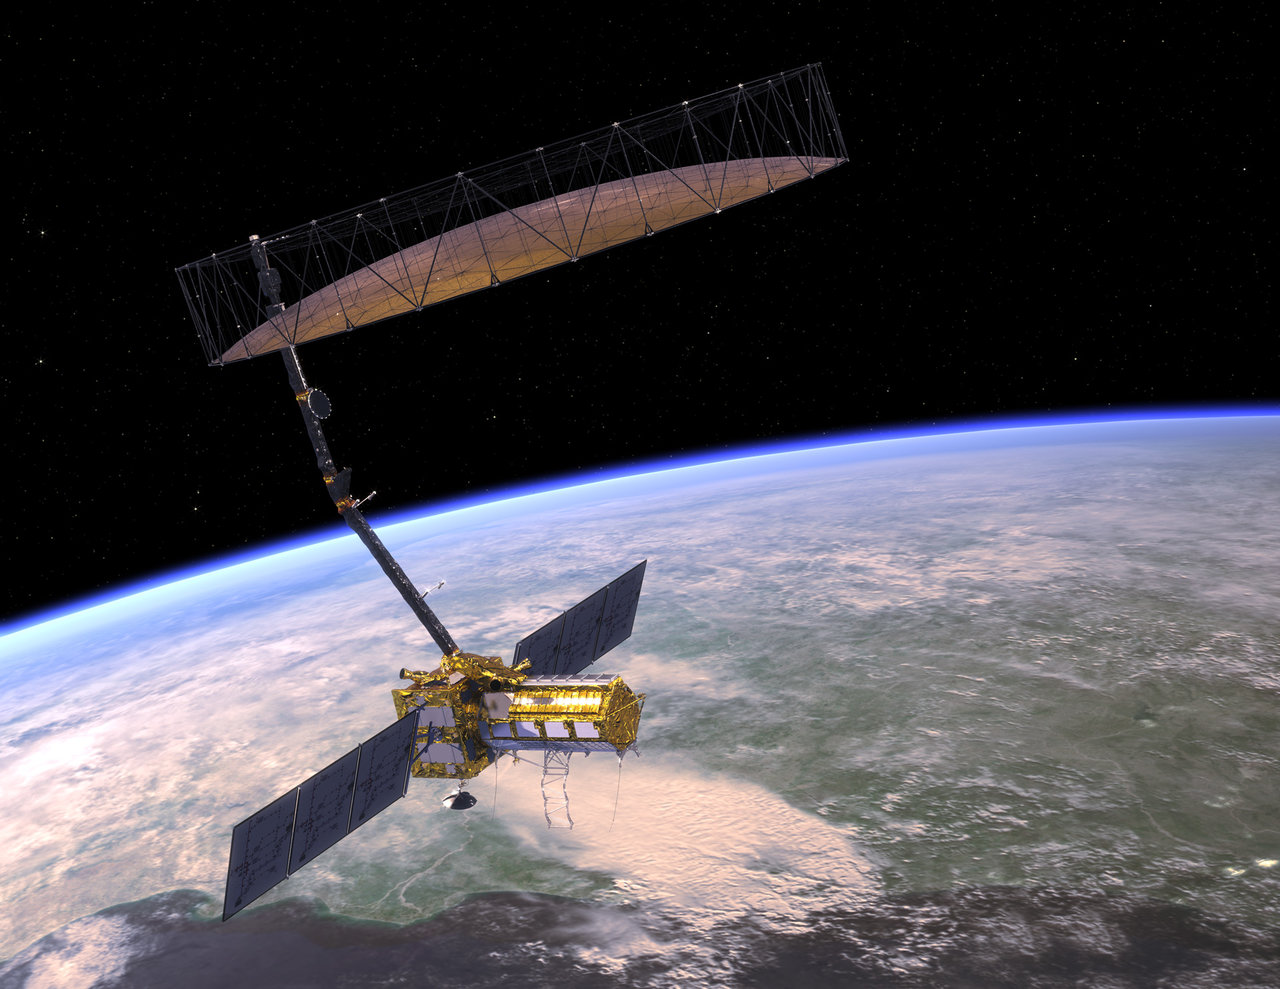
\includegraphics[scale=0.45]{Images/NISAR.jpg}
\end{figure}

\pagebreak

\section*{\Large REVISION HISTORY}

\begin{table}[h!]
\begin{center}
\begin{tabular} [0.9 \textwidth]{cl}
\hline \hline
\multicolumn{1}{c}{VERSION} & \multicolumn{1}{l}{REVISION NOTES} \\
\hline
PS1 & - Created document \\
    & - Added PS1 material \\
\hline
PS2 & - Added PS2 material \\
    & - Updated title page \\
    & - Updated moment of inertia for center of mass \\
\hline
PS3 & - Added PS3 material \\
    & - Updated title page \\
\hline
PS4 & - Added PS4 material \\
    & - Updated title page \\
    & - Switched to 312 Euler angles \\
\hline
PS5 & - Added PS5 material \\
    & - Updated title page \\
    & - Fix PS2 figure caption typos \\
    & - Fix PS4 figure numbering \\
\hline
PS6 & - Introduce Simulink model \\
    & - Added PS6 material \\
    & - Updated title page \\
    & - Fixed PS5 stability plot \\
\hline
PS7 & - Added PS7 material \\
    & - Updated title page \\
    & - Added PS5 RTN attitude and net torque plots \\
\hline
PS8 & - Added PS8 material \\
    & - Updated title page \\
\hline
PS9 & - Added PS9 material \\
    & - Updated title page \\
    & - Fixed advanced magnetic field model \\
\hline
PS10 & - Reformatted for final project submission \\
    & - Added magnetorquer actuator model \\
    & - Added desaturation mode \\
    & - Extended magnetic field model for accurate modeling of magnetorquer \\
    & - Addressed PS8 comments about covariance errors \\
\hline \hline
\end{tabular}
	\caption{Summary of project revisions.}
\end{center}
\end{table}
 
\newpage
\section*{\Large TABLE OF CONTENTS}
\makeatletter
\@starttoc{toc}
\makeatother
\newpage
%%%%%%%%%%%%%%%%%%%%%%%%%%%%%%%%%%%%%%%%%%%%%%%%%%%%%%%%%%%%%%%%%%%%%%%%%%%%%%%%%%%%%%%%%%%%%%%%%%%%%%%%%%%%%%%%%%%%%%%%%%%%%%%%%%%%%%%%%%%%%%%%%%%%%%%%%%%%%%%%%%%%%%%%%%%%%%%%%%%%%%%%%%%%%%%%%%%%%%%%%%%%%%%%%%%%%%%%%%%

% \section{\Large INTRODUCTION}

% \section{\Large PROBLEM SET 1}
\subsection{PROBLEM 1}
\textit{Select some key ADCS characteristics of your mission, including orbit (e.g., LEO, MEO, GEO, HEO, Interplanetary), target attitude (e.g., Sun pointing, Inertial pointing, Earth pointing, Resident Space Object pointing), attitude state representation (e.g., Euler angles, Gibbs vector, Quaternions Direction Cosine Matrix, Euler Axis/Angle), sensors suite (Gyros, Magnetometers, Star Trackers, Earth Sensor, Sun Sensor), actuator suite (Thrusters, Magnetorquers, Reaction Wheels, Momentum Wheel, Gravity Gradient).}

Our mission will utilize a satellite with synthetic aperture radar (SAR), designed to gather key remote sensing and environmental data for the Earth. The satellite will be in low Earth orbit (LEO) and use quaternions to describe its orientation, avoiding gimbal lock effects of other conventions. For state estimation, the spacecraft will require gyroscopes, star trackers, and a potentially a sun sensor. For actuation, the spacecraft will likely utilize thrusters, reaction wheels, and magnetorquers.

\subsection{PROBLEM 2}
\textit{Conduct survey of satellites which have characteristics similar to selected project. Use internet, publications, and books as resources.}

Space agencies such as NASA have been constructing SAR satellites to gather satellite images and data of Earth for over a decade. Additionally, there exist commercial entities also utilizing SAR in their spacecraft.

For example, Soil Moisture Active Passive (SMAP) is a NASA satellite launched in 2015 that utilizes L-band synthetic aperture radar (SAR) technology to measure soil moisture from LEO. This data has applications in climate change research climate change research applications (such as updating climate models) and some day-to-day activities (such as improving weather forecasts). SMAP is unique in that it had a large deployable reflector, held above the spacecraft body by a deployable boom \cite{SMAP}.

Companies EOS and Capella Space are also developing satellites that use SAR technology in the X-band and S-band frequencies for commercial applications ranging from agriculture to mining \cite{EOSSAR, Capella}. The commercial applicability of SAR is substantial, especially as SAR can penetrate cloud cover while generating high-resolution data, making it superior to many other forms of remote sensing technology. EOS claims to obtain resolution of up to 0.25 m, while Capella Space claims a capability of up to 0.5 m. These satellites all operate in LEO, which enables high-frequency monitoring of the Earth's surface.

NASA and ISRO have partnered to create a SAR satellite as well. The joint project between NASA JPL and ISRO has resulted in the NASA-ISRO Synthetic Aperture Radar (NISAR), a satellite that captures data in the L-band and S-band SAR frequencies \cite{NISARMission}. NISAR's high resolution will permit the detailed measurement of the Earth's surface, enabling better observation of changes in Earth's crust for disaster prevention and mitigation. NISAR will also support science goals such as monitoring ice sheets and the oceans, and its orbit is designed to cover the entire Earth every 12 days.

\subsection{PROBLEM 3}
\textit{Select preferred existing satellite and payload for project. Similarity is helpful, but not strictly required.}

We select the NASA JPL and ISRO NISAR mission as the mission on which to base our satellite. In the following section, we describe mission details and basic specifications. We simplify the satellite geometry and compute the center of mass and inertia tensor of the satellite. We will also analyze the satellite's external surfaces, which are relevant to disturbances such as atmospheric drag and solar radiation pressure.

\subsection{PROBLEM 4}
\textit{Collect basic information on mission, requirements, ADCS sensors and actuators, mechanical layout, mass, mass distribution, and inertia properties.}

NISAR is a joint Earth-observation satellite mission between NASA and ISRO. It is the first satellite to operate in two different Synthetic Aperture Radar (SAR) bands, incorportating both L- and S-band SAR instruments. Both frequencies can penetrate clouds for reliable data collection, but the L-band can also penetrate thicker vegetation that the S-band cannot. Uniquely, NISAR is intended to be used for a wide range of science objectives, including disaster response and agriculture \cite{NISARApps}.

NISAR ADCS requirements are \textless 273 arcseconds for pointing and \textless 500 m for orbit control \cite{Siqueira}. The satellite duty cycle is specified as \textgreater 30\%. NISAR will operate in LEO with nominal altitude of 747 km and 6 AM/6 PM orbit. NISAR's L- and S-band instruments operate at 24 cm and 12 cm wavelengths, respectively. NISAR collects terrestial SAR imagery with an image swatch of 240 km using a sweep approach. The science payload can also perform polarimetry, with the SAR incorporating multiple polarization modes.

\begin{figure}[H]
\centering
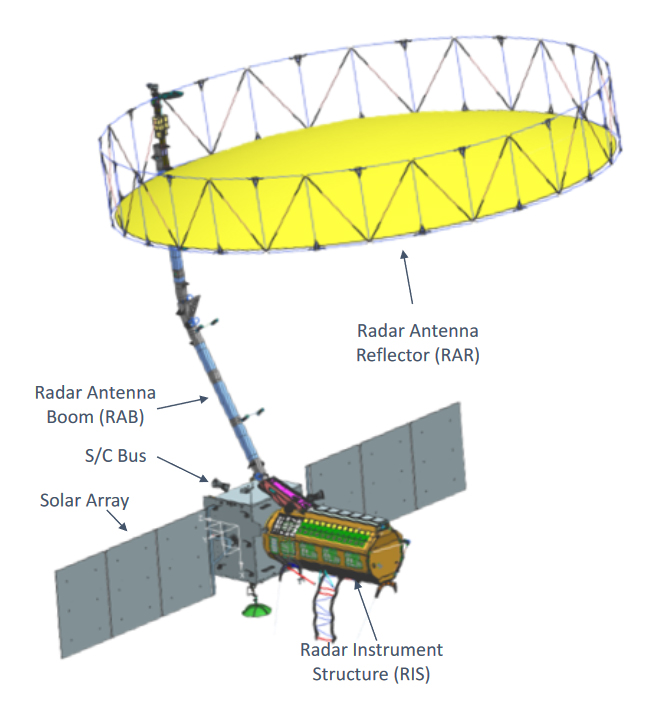
\includegraphics[scale=0.38]{Images/nisar_diagram.jpg}
\caption{The basic components of the NISAR satellite}
\label{NISAR Diagram}
\end{figure}

As shown in Figure \ref{NISAR Diagram}, NISAR's satellite consists of a 1.2 m x 1.8 m x 1.9 m spacecraft bus cuboid with a 1.2 m wide octagonal Radar Instrument Structure (RIS). The spacecraft bus includes ADCS hardware, power subsystem, and engineering payload, while the RIS houses hardware for the L- and S-band SAR. The satellite is powered by 23 m\textsuperscript{2} of solar panels, consisting of an array of two panels, one on each side of the satellite. Additionally, a 12 m diameter radar antenna is positioned above the body of the spacecraft, attached by a 9 m long boom. This boom consists of beams with 7 in x 7 in cross-section area \cite{NISARMission}.

Table \ref{tab:mass} contains mass properties of the satellite. Unfortunately, detailed mass distribution and inertia properties of NISAR are not openly available, so we provide estimates of mass distribution based on known overall component-level masses. We are given total masses for the bus structure and RIS, and we also know the masses of the payloads located within, allowing us to compute an accurate mass for these components \cite{NISARMission}. We estimate that solar panels have a mass of 23 kg each based on knowledge that NISAR's solar panels are 23 m\textsuperscript{2} and a typical solar panel mass per area is 2.06 kg/m\textsuperscript{2} \cite{SolarPanelMass}. We know that the entire radar antenna assembly has a mass of 292 kg, and we estimate that the reflector has a mass of approximately 100 kg based on a similar deployable SAR S- and L-band mesh antenna reflector \cite{L3Harris}. We will use these masses to compute center of mass and moments of inertia in the following section. For our model, we neglect the effects of the truss structure supporting the antenna reflector, instead modeling the entire RAR as just the disk-shaped reflector mesh.

\begin{longtable}{l|r}
\caption{Mass of NISAR components}
\label{tab:mass}\\
\textbf{Components}              & \multicolumn{1}{l}{\textbf{Mass [kg]}} \\ \hline
\endfirsthead
%
\endhead
%
Bus                              & 964.1                                      \\
Radar Instrument Structure (RIS) & 1375.9                                     \\
Solar Panel +y                   & 23                                         \\
Solar Panel -y                   & 23                                         \\
Radar Antenna Boom (RAB)         & 192                                        \\
Radar Antenna Reflector (RAR)    & 100                                       
\end{longtable}

Since NISAR is a remote sensing satellite requiring high attitude control performance, it has an ADCS system with an array of sensors and actuators. Sensors include star sensors, sun sensors, GPS, and a 3-axis gyroscope for roll, pitch, and yaw. For actuators, NISAR has four 50 N$\cdot$m reaction wheels mounted in tetrahedral configuration, three 565 and 350 A$\cdot$m\textsuperscript{2} magnetorquers, and fourteen thrusters (ten canted 11 N thrusters, one central 11 N thruster, and four 1 N thrusters for roll) \cite{NISARMission}.

\subsection{PROBLEM 5}
\textit{Simplify spacecraft geometry, make assumptions on mass distribution, e.g. splitting it in its core parts, define body axes (typically related to geometry and payload), compute moments of inertia and full inertia tensor w.r.t. body axes. Show your calculations.}

We simplify the spacecraft geometry into six components, each individually assumed to have uniform mass distribution. These components of the simplified geometry are: bus structure (including ADCS hardware and engineering payload), RIS (Radar Instrument Structure), RAB (radar antenna boom), RAR (radar antenna reflector), and two solar panels (identified as the +y solar panel and -y solar panel). The bus structure is modeled as a rectangular prism, while the RIS is modeled as an octagonal prism. The RAB is also modeled as a rectangular prism, while the RAR is modeled as a thin disk and the solar panels are modeled as thin rectangular plates. Within each geometry, our model assumes mass is distributed uniformly. From analyzing diagrams found in technical reports, we estimate that the RAR is tilted -3.87\degree{} about the y-axis (relative to the x-axis), while the RAB is modeled as a single beam with an angle approximately -18\degree{} from vertical (from the z-axis, about the y-axis in the x-z plane). Note that we have simplified the shape of the RAB from a beam of two angled segments to a single, straight beam.

We choose the body axes to have an origin at the center of the rectangular bus. This configuration is chosen because the bus houses the ADCS hardware, including actuators and sensors. The x-axis points in the direction of the RIS, and the z-axis points up vertically, normal to the upper surface of the bus. See Figure \ref{fig:MATLAB_model} for a visual depiction of the body axes relative to the spacecraft.

We compute the center of mass after extracting the centroid of each component. The mass of each component is previously found in Table \ref{tab:mass}. The centroid of each component is listed in Table \ref{tab:centroid}.

\begin{longtable}{l|r|r|r}
\caption{Component centroids [m]}
\label{tab:centroid}\\
\textbf{Part} & \multicolumn{1}{l}{\textbf{x}} & \multicolumn{1}{l}{\textbf{y}} & \multicolumn{1}{l}{\textbf{z}} \\ \hline
\endfirsthead
%
\endhead
%
Bus      & 0     & 0    & 0    \\
RIS      & 1.85  & 0    & 0    \\
Panel +y & 0     & 3.9  & 0    \\
Panel -y & 0     & -3.9 & 0    \\
RAB      & -0.899 & 0    & 5.194 \\
RAR      & 4.283   & 0    & 8.308
\end{longtable}

The center of mass can be found by taking the weighted average of each component centroid, weighted by the mass of each component. The center of mass formula is:

\begin{equation*}
    \Vec{r}_{cm} = \frac{\sum m_{i} \Vec{r}_{i}}{\sum m_{i}}
\end{equation*}

This yields a result for center of mass at $\qty[parse-numbers = false]{[1.046, 0, 0.683]}{\metre}$ relative to the origin we defined. We created the following MATLAB script to compute the center of mass from a CSV file containing centroid and mass data.

\lstinputlisting{src/computeCM.m}

We compute the moment of inertia of the satellite, finding an inertia tensor in our body axes. To do this, we break the satellite into individual components, first finding the moment of inertia about the center of mass of each component. We then compute the moment of inertia of the entire satellite about the body axes by using parallel axis theorem and combining all the components.

To compute the moment of inertia, we need the following geometric properties of each component:

\begin{longtable}{l|r|r|r|r|r}
\caption{Dimensions of modeled components [m]}
\label{tab:dimensions}\\
\textbf{Part} & \textbf{L (x-dim)} & \textbf{W (y-dim)} & \textbf{H (z-dim)} & \textbf{S (oct. side length)} & \textbf{R (radius)} \\ \hline
\endfirsthead
%
\endhead
%
Bus &  & 1.8 & 1.9 & - & - \\
RIS & 2.5 & - & - & 0.459 & - \\
Panel +y & - & 6 & 1.9 & - & - \\
Panel -y & - & 6 & 1.9 & - & - \\
RAB & 0.1778 & 0.1778 & 9 & - & - \\
RAR & - & - & - & - & 6
\end{longtable}

For the bus, we choose to model the geometry as a rectangular prism. Since the bus is aligned with the body axes, we obtain a diagonal inertia tensor:

\begin{align*}
I_{bus} &=
\begin{bmatrix}
I_{xx} & 0 & 0 \\
0 & I_{yy} & 0 \\
0 & 0 & I_{zz}
\end{bmatrix} \\
&=
\begin{bmatrix}
m \frac{W^{2} + H^{2}}{12} & 0 & 0 \\
0 & m \frac{L^{2} + H^{2}}{12} & 0 \\
0 & 0 & m \frac{L^{2} + W^{2}}{12} 
\end{bmatrix} \\
&=
\qty[parse-numbers = false]{
\begin{bmatrix}
550.340 & 0 & 0 \\
0 & 405.725 & 0 \\
0 & 0 & 375.9993 
\end{bmatrix}
}{\kilogram\metre\squared}
\end{align*}

For the solar panels, we approximate their geometry as a flat plate. These axes are also aligned, so the tensor can be diagonal.

\begin{align*}
I_{panel} &=
\begin{bmatrix}
I_{xx} & 0 & 0 \\
0 & I_{yy} & 0 \\
0 & 0 & I_{zz}
\end{bmatrix} \\
&=
\begin{bmatrix}
m \frac{W^{2} + H^{2}}{12} & 0 & 0 \\
0 & m \frac{H^{2}}{12} & 0 \\
0 & 0 & m \frac{W^{2}}{12} 
\end{bmatrix} \\
&=
\qty[parse-numbers = false]{
\begin{bmatrix}
75.919 & 0 & 0 \\
0 & 6.919 & 0 \\
0 & 0 & 69 
\end{bmatrix}
}{\kilogram\metre\squared}
\end{align*}

For the RIS, we model the geometry as an octagonal prism. For the moment of inertia about the axisymmetric axis of the octagon, we use the formula $m \left(\frac{S^{2}}{24} + \frac{a^{2}}{2}\right)$, where $S$ is the side length and $a$ is the apothem length, where the apothem is the perpendicular length from a side of the octagon to the center \cite{McCarron}. When calculating the moment of inertia about the non-axisymmetric axes, we approximate the geometry as a cylinder with radius equal to the average of the octagonal radius (distance from center to vertex) and the apothem. As will be shown later, this approximation yields a very close result to the inertia tensor generated from the CAD model.

\begin{align*}
I_{RIS} &=
\begin{bmatrix}
I_{xx} & 0 & 0 \\
0 & I_{yy} & 0 \\
0 & 0 & I_{zz}
\end{bmatrix} \\
&=
\begin{bmatrix}
m \left(\frac{S^{2}}{24} + \frac{a^{2}}{2}\right) & 0 & 0 \\
0 & m \left(\frac{L^{2}}{12} + \frac{R_{avg}^{2}}{4}\right) & 0 \\
0 & 0 & m \left(\frac{L^{2}}{12} + \frac{R_{avg}^{2}}{4}\right) 
\end{bmatrix} \\
&=
\qty[parse-numbers = false]{
\begin{bmatrix}
223.268 & 0 & 0 \\
0 & 831.089 & 0 \\
0 & 0 & 831.089 
\end{bmatrix}
}{\kilogram\metre\squared}
\end{align*}

For the RAB, we first model the geometry as a rectangular prism. We also must rotate the inertia tensor to match the orientation of the body axes, as the RAB itself is rotated relative to the bus about the y-axis by -18\degree{} from vertical (z-axis).

\begin{align*}
I_{RAB} &=
\begin{bmatrix}
I_{xx} & 0 & 0 \\
0 & I_{yy} & 0 \\
0 & 0 & I_{zz}
\end{bmatrix} \\
&=
\begin{bmatrix}
m \frac{W^{2} + H^{2}}{12} & 0 & 0 \\
0 & m \frac{L^{2} + H^{2}}{12} & 0 \\
0 & 0 & m \frac{L^{2} + W^{2}}{12} 
\end{bmatrix} \\
&=
\qty[parse-numbers = false]{
\begin{bmatrix}
1296.506 & 0 & 0 \\
0 & 1296.506 & 0 \\
0 & 0 & 1.012 
\end{bmatrix}
}{\kilogram\metre\squared}
\end{align*}

We apply the rotation to the inertia tensor using a rotation matrix about the y-axis. Note that doing so results in non-zero products of inertia, meaning our principal axes will not be aligned with our body axes.

\begin{align*}
I_{RAB,rotated} &= R_{y}(-18\degree) I_{RAB} R_{y}^{\intercal}(-18\degree) \\
&=
\qty[parse-numbers = false]{
\begin{bmatrix}
1172.797 & 0 & 380.736 \\
0 & 1296.506 & 0 \\
380.736 & 0 & 124.720
\end{bmatrix}
}{\kilogram\metre\squared}
\end{align*}

Finally, we model the RAR as a flat disk. Similar to the RAB, we must rotate the inertia tensor to match the orientation of the body axes.

\begin{align*}
I_{RAR} &=
\begin{bmatrix}
I_{xx} & 0 & 0 \\
0 & I_{yy} & 0 \\
0 & 0 & I_{zz}
\end{bmatrix} \\
&=
\begin{bmatrix}
m \frac{R^{2}}{4} & 0 & 0 \\
0 & m \frac{R^{2}}{4} & 0 \\
0 & 0 & m \frac{R^{2}}{2} 
\end{bmatrix} \\
&=
\qty[parse-numbers = false]{
\begin{bmatrix}
900 & 0 & 0 \\
0 & 900 & 0 \\
0 & 0 & 1800 
\end{bmatrix}
}{\kilogram\metre\squared}
\end{align*}

Applying a rotation:

\begin{align*}
I_{RAR,rotated} &= R_{y}(-3.87\degree) I_{RAR} R_{y}^{\intercal}(-3.87\degree) \\
&=
\qty[parse-numbers = false]{
\begin{bmatrix}
904.100 & 0 & -60.605 \\
0 & 900 & 0 \\
-60.605 & 0 & 1795.900
\end{bmatrix}
}{\kilogram\metre\squared}
\end{align*}

Now, we use parallel axis theorem to compute the moment of inertia of each component about the body axes at the specified origin. We can use the following displacement tensor,

\begin{equation*}
D =
\begin{bmatrix}
y^{2} + z^{2} & -xy & -xz \\
-yx & x^{2} + z^{2} & -yz \\
-zx & -yz & x^{2} + y^{2}
\end{bmatrix},
\end{equation*}

where $x$, $y$, $z$ are the coordinates of the center of mass of the component, giving the moment of inertia about a new point:

\begin{equation*}
    I' = I_{c} + mD
\end{equation*}

Performing the parallel axis theorem on each component and summing the inertia tensors, we obtain the following inertia tensor for the entire spacecraft:

\begin{equation*}
I_{NISAR,body} =
\qty[parse-numbers = false]{
\begin{bmatrix}
15783.996 & 0 & -2341.659 \\
0 & 22227.752 & 0 \\
-2341.659 & 0 & 10663.970
\end{bmatrix}
}{\kilogram\metre\squared}
\end{equation*}

Compare this with the inertia tensor computed by SolidWorks CAD software:

\begin{equation*}
I_{NISAR,body} =
\qty[parse-numbers = false]{
\begin{bmatrix}
15780.361 & 0 & -2336.285 \\
0 & 22225.721 & 0 \\
-2336.285 & 0 & 10665.796
\end{bmatrix}
}{\kilogram\metre\squared}
\end{equation*}

The errors are 0.0230\%, 0.00914\%, 0.0171\%, and 0.230\% for $I_{xx}$, $I_{yy}$, $I_{zz}$, and $I_{xz}$, respectively. We created the following MATLAB script to compute the inertia tensor.

\lstinputlisting{src/computeMOI.m}

\subsection{PROBLEM 6}
\textit{Discretize your spacecraft through its outer surfaces (geometry). Develop a Matlab/Simulink function to handle barycenter (geometry, no mass distribution) coordinates, size, and unit vectors normal to each outer surface of the spacecraft in body frame. You can list all this information in a Matrix. This will be essential later on to compute environmental torques acting on the spacecraft from forces, surface orientation, and the vectors connecting the satellite’s center of mass to each surface’s center of mass.}

For the purpose of discretizing the spacecraft into surfaces, we consider the outer faces of the bus, RIS, and RAB. We also consider the faces of the solar panels and RAR, which are modeled as thin plates. The centroid (barycenter) coordinates and area for each surface are obtained using the surface properties tool in SolidWorks, and a unit normal vector is manually computed based on the orientation of the surface. We then enter this data into a CSV file, which can be read into MATLAB using the following function:

\lstinputlisting{src/surfaces.m}

This function stores the data into arrays of barycenter coordinates, unit normal vector components, and area. Each row of an array corresponds to a particular surface. The data is shown in Table \ref{tab:surfaces}, annotated with the identity of each surface.

\begin{longtable}{l|r|r|r|r|r|r|r}
\caption{Surface parameters}
\label{tab:surfaces}\\
 &
  \multicolumn{3}{c}{\textbf{Barycenter [m]}} &
  \multicolumn{3}{c}{\textbf{Normal}} &
  \multicolumn{1}{l}{} \\
\endfirsthead
%
\endhead
%
\textbf{Surface} &
  \multicolumn{1}{l}{\textbf{x}} &
  \multicolumn{1}{l}{\textbf{y}} &
  \multicolumn{1}{l}{\textbf{z}} &
  \multicolumn{1}{l}{\textbf{x}} &
  \multicolumn{1}{l}{\textbf{y}} &
  \multicolumn{1}{l}{\textbf{z}} &
  \multicolumn{1}{l}{\textbf{Area [m\textsuperscript{2}]}} \\ \hline
Bus front, minus RIS (+x) & 0.6   & 0     & 0     & 1      & 0      & 0      & 2.4   \\
Bus rear (-x)                  & -0.6  & 0     & 0     & -1     & 0      & 0      & 3.42  \\
Bus side (+y)                  & 0     & 0.9   & 0     & 0      & 1      & 0      & 2.28  \\
Bus side (-y)                  & 0     & -0.9  & 0     & 0      & -1     & 0      & 2.28  \\
Bus top (+z)                   & 0     & 0     & 0.95  & 0      & 0      & 1      & 2.16  \\
Bus bottom (-z)                & 0     & 0     & -0.95 & 0      & 0      & -1     & 2.16  \\
RIS front (+x)                 & 3.1   & 0     & 0     & 1      & 0      & 0      & 1.02  \\
RIS top (+z)                   & 1.85  & 0     & 0.55  & 0      & 0      & 1      & 1.15  \\
RIS bottom (-z)                & 1.85  & 0     & -0.55 & 0      & 0      & -1     & 1.15  \\
RIS side (+y)                  & 1.85  & 0.55  & 0     & 0      & 1      & 0      & 1.15  \\
RIS side (-y)                  & 1.85  & -0.55 & 0     & 0      & -1     & 0      & 1.15  \\
RIS angle face (y-z I)         & 1.85  & 0.39  & 0.39  & 0      & 0.707  & 0.707  & 1.15  \\
RIS angle face (y-z II)        & 1.85  & -0.39 & 0.39  & 0      & -0.707 & 0.707  & 1.15  \\
RIS angle face (y-z III)       & 1.85  & -0.39 & -0.39 & 0      & -0.707 & -0.707 & 1.15  \\
RIS angle face (y-z IV)        & 1.85  & 0.39  & -0.39 & 0      & 0.707  & -0.707 & 1.15  \\
Panel +y front (+x)            & 0     & 3.9   & 0     & 1      & 0      & 0      & 11.4  \\
Panel +y rear (-x)             & 0     & 3.9   & 0     & -1     & 0      & 0      & 11.4  \\
Panel -y front (+x)            & 0     & -3.9  & 0     & 1      & 0      & 0      & 11.4  \\
Panel -y rear (-x)             & 0     & -3.9  & 0     & -1     & 0      & 0      & 11.4  \\
RAB front (x-z, +x)            & -0.81 & 0     & 5.21  & 0.951  & 0      & 0.309  & 1.6   \\
RAB rear (x-z, -x)             & -0.99 & 0     & 5.18  & -0.951 & 0      & -0.309 & 1.6   \\
RAB side (+y)                  & -0.9  & -0.09 & 5.19  & 0      & 1      & 0      & 1.6   \\
RAB side (-y)                  & -0.9  & 0.09  & 5.19  & 0      & -1     & 0      & 1.6   \\
RAB top (+z)                   & -2.31 & 0     & 9.47  & 0      & 0      & 1      & 0.03  \\
RAR top (+z)                   & 4.28  & 0     & 8.31  & -0.067 & 0      & 0.998  & 113.1 \\
RAR bottom (-z)                & 4.28  & 0     & 8.31  & 0.067  & 0      & -0.998 & 113.1
\end{longtable}

\subsection{PROBLEM 7}
\textit{At this stage you should have a simple 3D model of your spacecraft including geometry and mass properties of each element. Plot body axes (triad) in 3D superimposed to spacecraft 3D model.}



A 3D model of the spacecraft is shown in Figure \ref{fig:complex_model}. The model shown is a screen capture from the SolidWorks CAD software.

\begin{figure}[H]
\centering
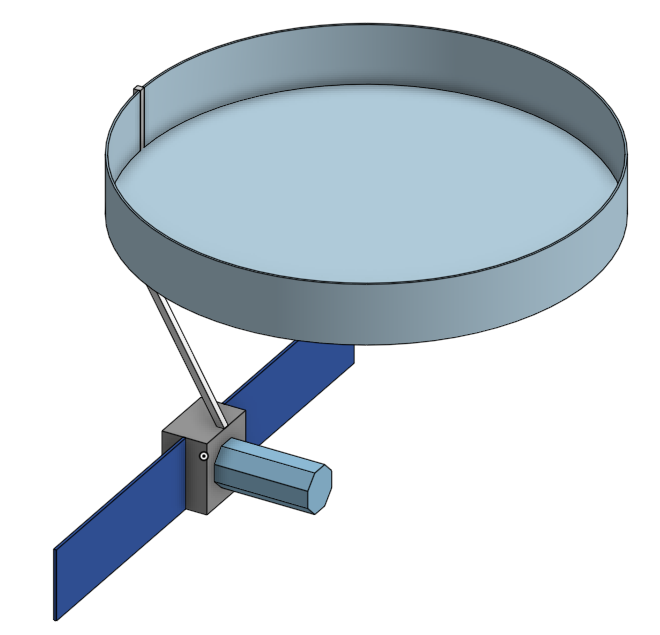
\includegraphics[scale=0.4]{Images/ps1_complex_model.png}
\caption{A 3D model of the satellite}
\label{fig:complex_model}
\end{figure}


We also show a simplified model of the spacecraft in Figure \ref{fig:simple_model}. This is the model we use to compute our mass and surface properties.

\begin{figure}[H]
\centering
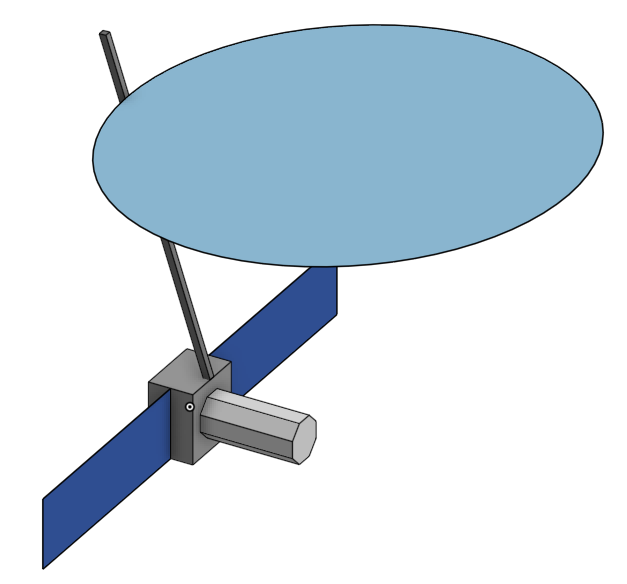
\includegraphics[scale=0.4]{Images/ps1_simple_model.png}
\caption{A 3D model of the simplified satellite geometry}
\label{fig:simple_model}
\end{figure}

We also plot the model in MATLAB by importing an STL version of the CAD model. We show the body axes in Figure \ref{fig:MATLAB_model}, with the origin chosen as the center of the spacecraft bus.

\begin{figure}[H]
\centering
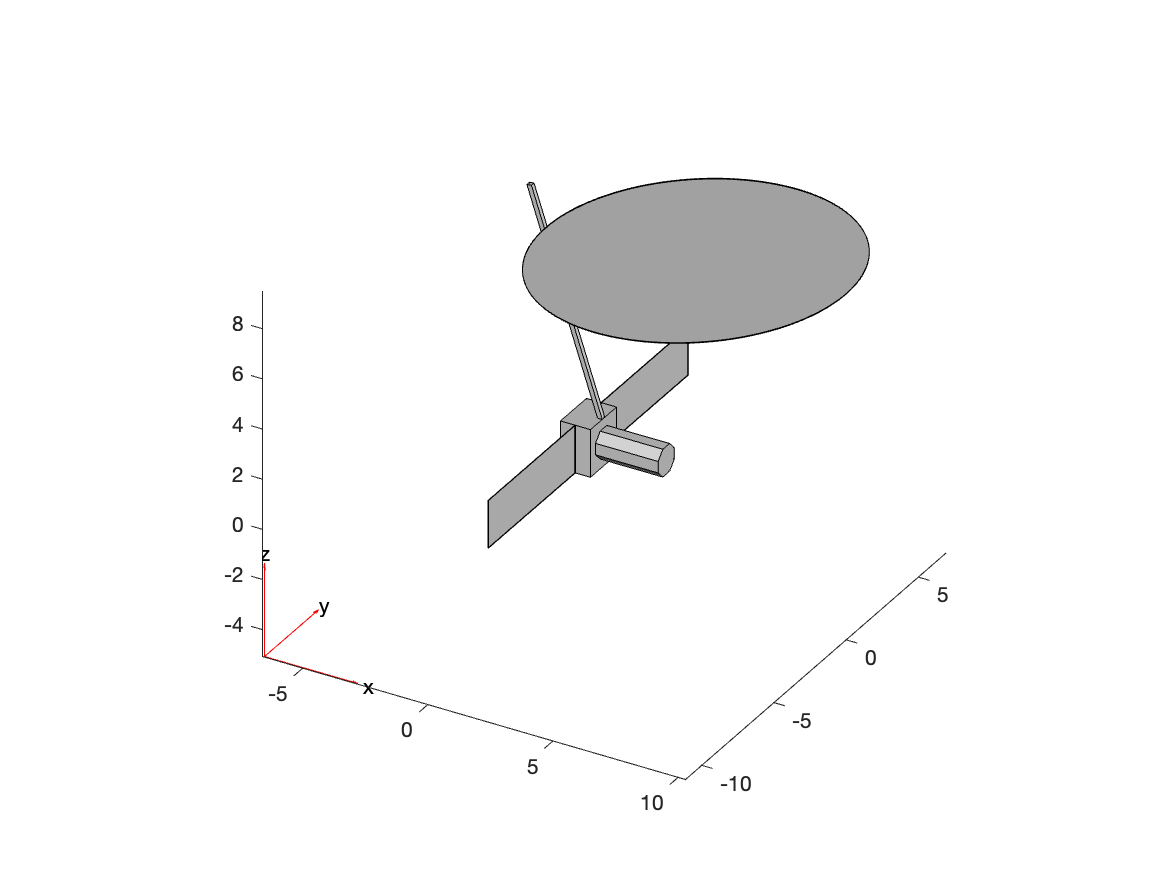
\includegraphics[scale=0.7]{Images/ps1_model.png}
\caption{Satellite model in MATLAB with body axes shown}
\label{fig:MATLAB_model}
\end{figure}



% \section{\Large PROBLEM SET 2}
\subsection{PROBLEM 1}
\textit{Define orbit initial conditions and make sure you can propagate the orbit of the satellite over multiple orbits using either a Keplerian propagator or a numerical integration scheme (see AA279A material). Best would be to use a numerical integrator, so that you can later try to feed the same environmental forces for orbit propagation which are applied for attitude propagation (very cool!).}

From the science users' handbook, we obtain the following orbital elements \cite{NISARHandbook}.

\begin{table}[H]
\begin{tabular}{lllllll}
\textbf{OE} & \textit{a} & \textit{e} & \textit{i} & \textit{$\Omega$} & \textit{$\omega$} & \textit{$\nu$} \\ \hline
\textbf{Value} & 7125.48662 km & 0.0011650 & 98.40508$\degree$ & -19.61601$\degree$ & 89.99764$\degree$ & -89.99818$\degree$
\end{tabular}
\end{table}

We convert these using a MATLAB function into ECI coordinates that can be fed into a numerical orbital propagator. Notice that we first convert the orbital elements a, e, and $\nu$ into perifocal (PQW) coordinates, using a and e to find the semi-latus rectum and a, e, and $\nu$ to find the distance to the central body (Earth). Then, we perform a series of rotations on these coordinates parameterized by $\omega$, i, and $\Omega$ to obtain new coordinates in the ECI frame.

\lstinputlisting{src/oe2eci.m}

Then, we can numerically propagate in MATLAB using \texttt{ode113} using a function that computes the time derivative of the ECI state. This is accomplished simply by setting the time derivative of position equal to the velocity portion of the state and setting the time derivative of velocity equal to an acceleration computed using the law of universal gravitation. Note that while our propagator does not include disturbance forces, it will be easy to incorporate these later. See the appendix corresponding to Problem Set 2 for application of \texttt{ode113}.

\lstinputlisting{src/orbitSimple.m}

Now, we plot the trajectory for one orbit in Figure \ref{fig:simple_propagator}. Plotting multiple orbits (for example, over 12 days) yields the same plot, as \texttt{ode113} is very stable for this application.

\begin{figure}[H]
\centering
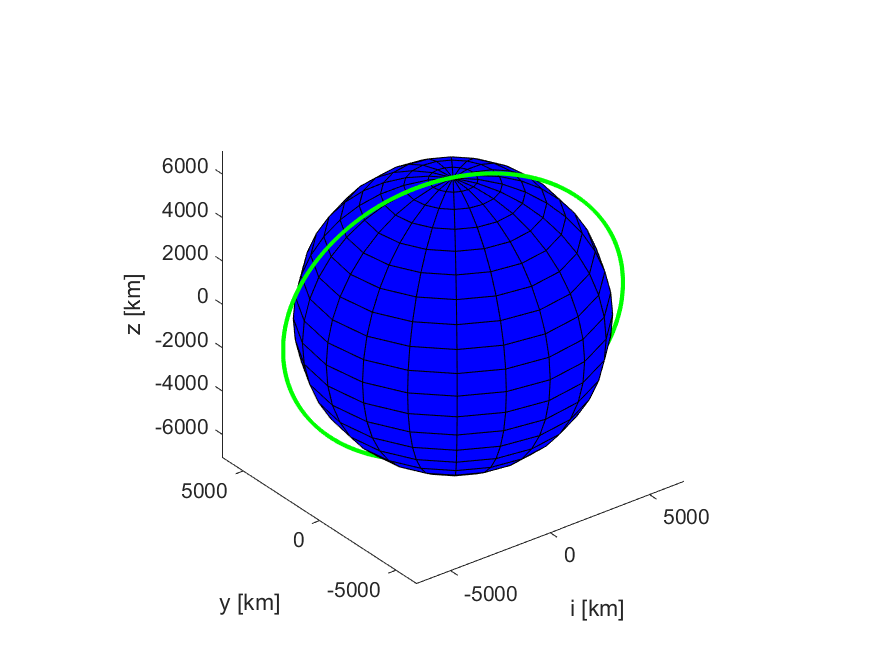
\includegraphics[scale=0.7]{Images/ps2_problem1.png}
\caption{A single orbit for NISAR in ECI coordinates (no perturbations)}
\label{fig:simple_propagator}
\end{figure}


\subsection{PROBLEM 2}
\textit{In general the body axes are not the principal axes. Identify principal axes through the eigenvector/eigenvalue problem discussed in class and compute the rotation matrix from body to principal axes.}

The unit vectors of the principal axes with respect to the body axes ($\Vec{e}_i$) and the inertia tensor in the principal axes ($I_i$) can be found by taking the eigenvalue decomposition of the inertia tensor in the body axis. This can be seen in the two equations below.

\begin{equation*}
    I_i \cdot \Vec{e}_i = I_i \cdot \Vec{I}_{body} \\ \hspace{1cm} i = x, y, z
\end{equation*}

\begin{align*}
\Vec{I}_{principal} &= 
    \begin{bmatrix}
    I_x & 0 & 0 \\
    0 & I_y & 0 \\
    0 & 0 & I_z 
    \end{bmatrix}
= 
\qty[parse-numbers = false]{
    \begin{bmatrix}
    7707.07 & 0 & 0 \\
    0 & 14563.2 & 0 \\
    0 & 0 & 18050.4 
    \end{bmatrix}
}{\kilogram\metre\squared}
\end{align*}

We follow convention $I_z > I_y > I_x$ for defining principal axes.

The unit vectors of the principal axes ($\Vec{e}_i$) can then be used to find the rotation matrix ($\Vec{R}$), as shown below.

\begin{align*}
\Vec{R} &= 
    \begin{bmatrix}
    \Vec{e}_x & \Vec{e}_y & \Vec{e}_z 
    \end{bmatrix}
= 
    \begin{bmatrix}
    -0.06278 & -0.99803 & 0 \\
    0 & 0 & 1 \\
    -0.99803 & 0.06278 & 0 
    \end{bmatrix} \\
    \Vec{I}_{body} &= \Vec{R} \Vec{I}_{principal} \Vec{R}^{\intercal}
\end{align*}


\subsection{PROBLEM 3}
\textit{At this stage you should have a simple 3D model of your spacecraft including geometry and mass properties of each element. This includes at least two coordinate systems, body and principal axes respectively, and the direction cosine matrix between them. Plot axes of triads in 3D superimposed to spacecraft 3D model.}

\begin{figure}[H]
\centering
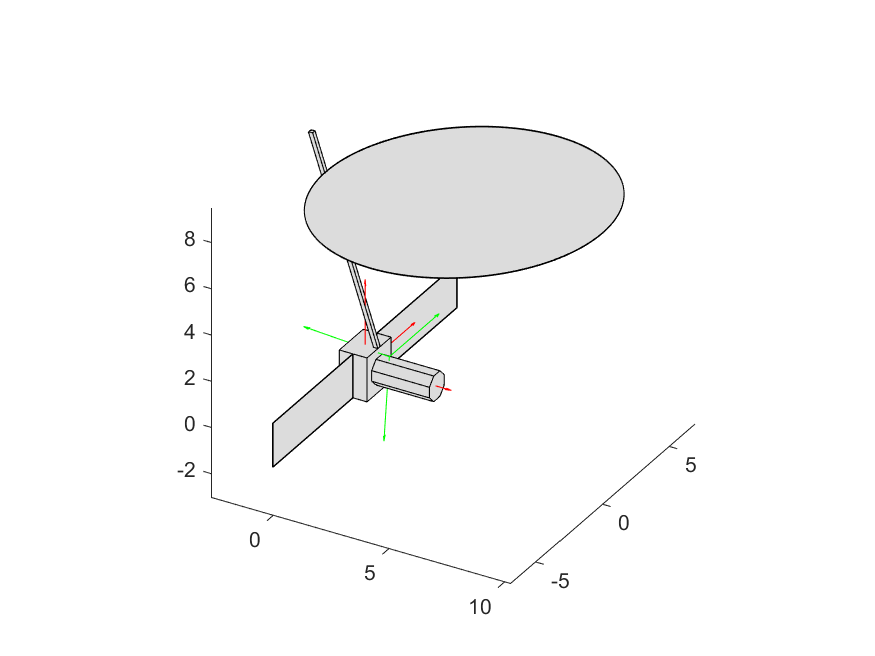
\includegraphics[scale=0.7]{Images/ps2_model.png}
\caption{Principal axes at center of mass (green) and body axes at origin (red)}
\label{fig:ps2_model}
\end{figure}


\subsection{PROBLEM 4}
\textit{Program Euler equations in principal axes (e.g. in Matlab/Simulink). No external torques.}

We use the following equations with zero external moments ($M_{x}, M_{y}, M_{z} = 0$).

\begin{align*}
    I_{x} \Dot{\omega}_{x} + (I_{z} - I_{y}) \omega_{y} \omega_{z} &= M_{x} \\
    I_{y} \Dot{\omega}_{y} + (I_{x} - I_{z}) \omega_{z} \omega_{x} &= M_{y} \\
    I_{z} \Dot{\omega}_{z} + (I_{y} - I_{x}) \omega_{x} \omega_{y} &= M_{z}
\end{align*}

\lstinputlisting{src/eulerEquation.m}


\subsection{PROBLEM 5}
\textit{Numerically integrate Euler equations from arbitrary initial conditions ($\omega<\qty{10}{\degree/\second}$, $\omega_{i}\neq0$). Multiple attitude revolutions.}

We choose arbitrary initial conditions $\omega_{x} = \qty{8}{\degree\per\second}$, $\omega_{y} = \qty{4}{\degree\per\second}$, and $\omega_{z} = \qty{6}{\degree\per\second}$. The results of numerical integration using \texttt{ode113} are shown in Figure \ref{fig:ps2_euler_equations}.

\begin{figure}[H]
\centering
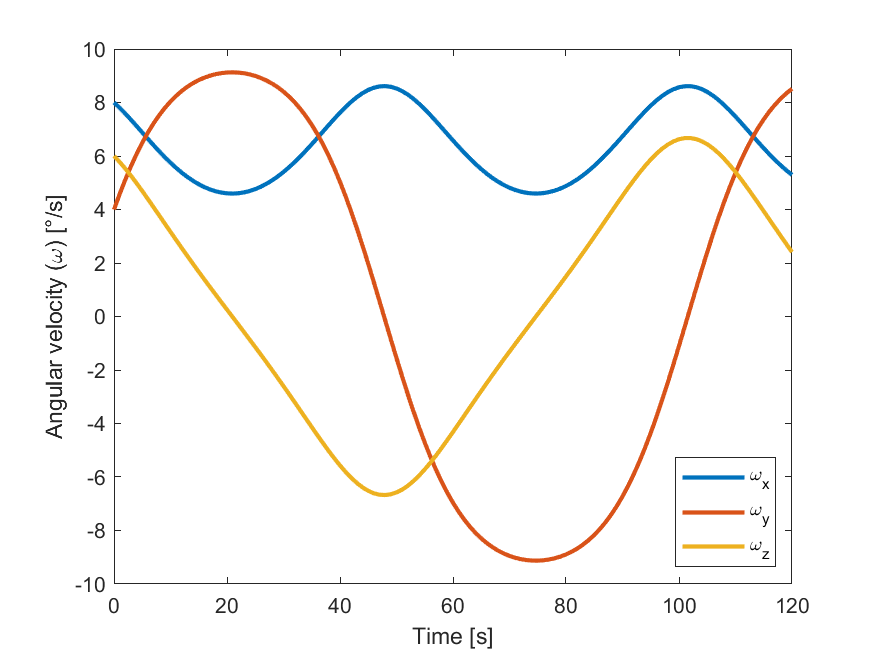
\includegraphics[scale=0.6]{Images/ps2_euler_equations.png}
\caption{Results from numerical integration of Euler equations}
\label{fig:ps2_euler_equations}
\end{figure}


\subsection{PROBLEM 6}
\textit{Plot rotational kinetic energy and momentum ellipsoids in 3D (axis equal) corresponding to chosen initial conditions. Verify that semi-axis of ellipsoids corresponds to theoretical values.}

For the energy ellipsoid, we compute our surface using rotational kinetic energy based on initial conditions and principal axes inertia tensor.

\begin{align*}
    &2T = \omega_{x}^{2} I_{x} + \omega_{y}^{2} I_{y} + \omega_{z}^{2} I_{z} \\
    &\frac{\omega_{x}^{2}}{2T/I_{x}} + \frac{\omega_{y}^{2}}{2T/I_{y}} + \frac{\omega_{z}^{2}}{2T/I_{z}} = 1
\end{align*}

For the given initial conditions, we get semi-major axes of the following lengths: $\omega_{x} = \qty{0.2332}{\radian\per\second}$, $\omega_{y} = \qty{0.1697}{\radian\per\second}$, and $\omega_{z} = \qty{0.1524}{\radian\per\second}$. These values make sense given the equation for the energy ellipsoid.

Similarly, we compute our surface for the momentum ellipsoid with angular momentum based on our initial conditions and the principal axes inertia tensor.

\begin{align*}
    &L = \omega_{x}^{2} I_{x}^{2} + \omega_{y}^{2} I_{y}^{2} + \omega_{z}^{2} I_{z}^{2} \\
    &\frac{\omega_{x}^{2}}{(L/I_{x})^{2}} + \frac{\omega_{y}^{2}}{(L/I_{y})^{2}} + \frac{\omega_{z}^{2}}{(L/I_{z})^{2}} = 1
\end{align*}

For the given initial conditions, we get semi-major axes of the following lengths: $\omega_{x} = \qty{0.3115}{\radian\per\second}$, $\omega_{y} = \qty{0.1649}{\radian\per\second}$, and $\omega_{z} = \qty{0.1330}{\radian\per\second}$. These values make sense given the equation for the momentum ellipsoid and are shown in the plots below.

We plot the energy ellipsoid in Figure \ref{fig:ps2_problem6_energy} and the momentum ellipsoid in Figure \ref{fig:ps2_problem6_momentum}.

\begin{figure}[H]
\centering
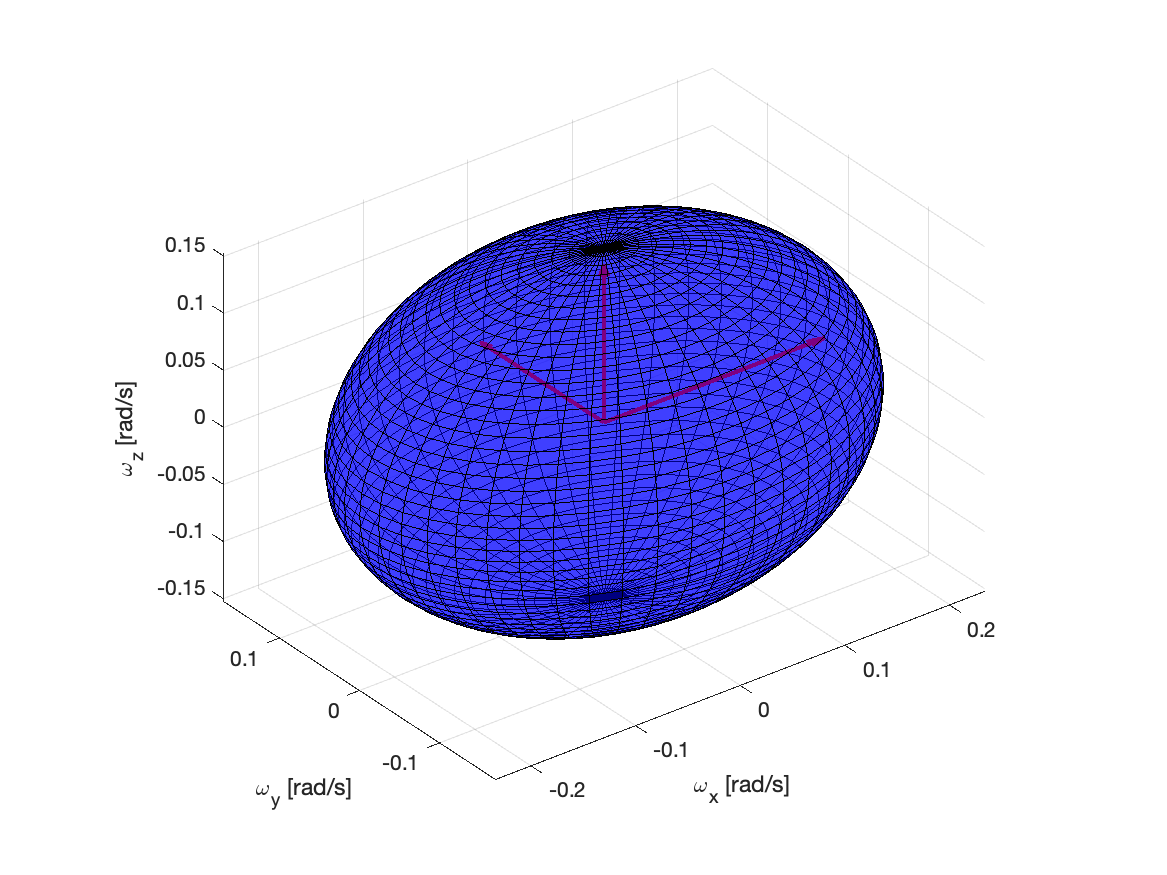
\includegraphics[scale=0.5]{Images/ps2_problem6_energy.png}
\caption{Energy ellipsoid with axes in red}
\label{fig:ps2_problem6_energy}
\end{figure}

\begin{figure}[H]
\centering
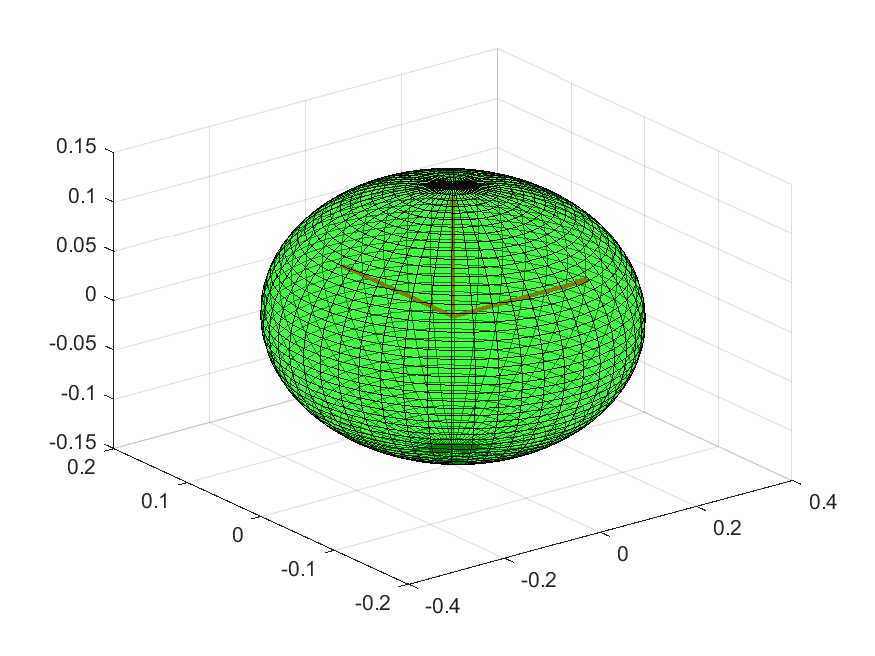
\includegraphics[scale=0.5]{Images/ps2_problem6_momentum.png}
\caption{Momentum ellipsoid with axes in red}
\label{fig:ps2_problem6_momentum}
\end{figure}


\subsection{PROBLEM 7}
\textit{Plot polhode in same 3D plot. Verify that it is the intersection between the ellipsoids.}

For a polhode plot to be real, the condition below must be verified.

\begin{equation*}
    I_x < \frac{L^2}{2T} < I_z
\end{equation*}

Based on previously calculated values ($I_x = 7707.1$, $\frac{L^2}{2T} = 13752.1$, $I_z = 18050.4$) we can verify that the polhode here will be real.

Figure \ref{fig:ps2_problem8} shows that the polhode is indeed the intersection between the ellipsoids.

\begin{figure}[H]
\centering
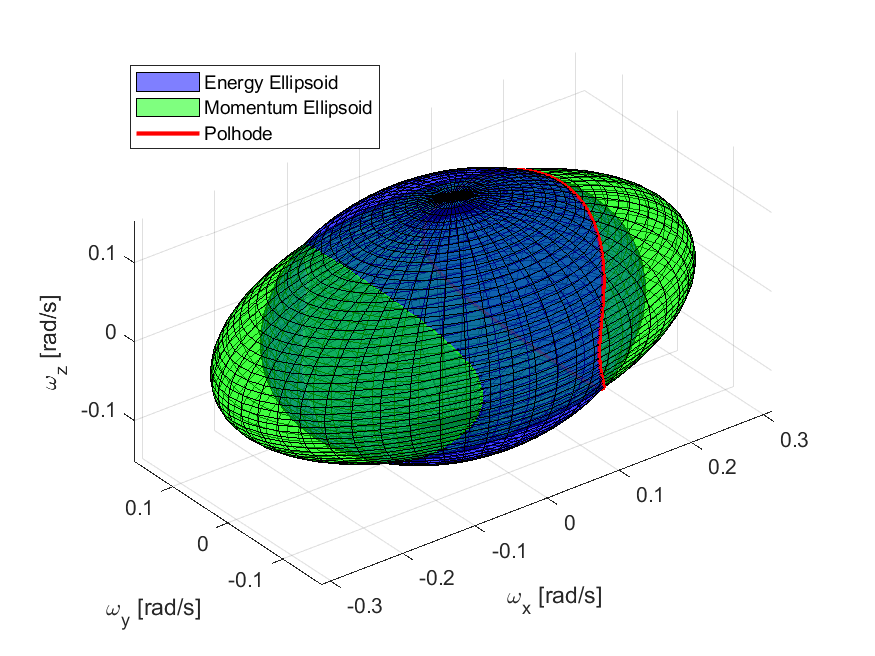
\includegraphics[scale=0.65]{Images/ps2_problem7.png}
\caption{Energy and momentum ellipsoids with polhode}
\label{fig:ps2_problem7}
\end{figure}

\subsection{PROBLEM 8}
\textit{Plot polhode in three 2D planes identified by principal axes (axis equal). Verify that shapes of resulting conic sections correspond to theory.}

The polhode conic sections in Figure \ref{fig:ps2_problem8} match expected theory. The polhode as seen along the x-axis is an ellipse, while the polhode along the y-axis is a hyperbola. We also see that when seen along the z-axis, the polhode also forms an ellipse, shown as a half-ellipse in our plot.

\begin{figure}[H]
\centering
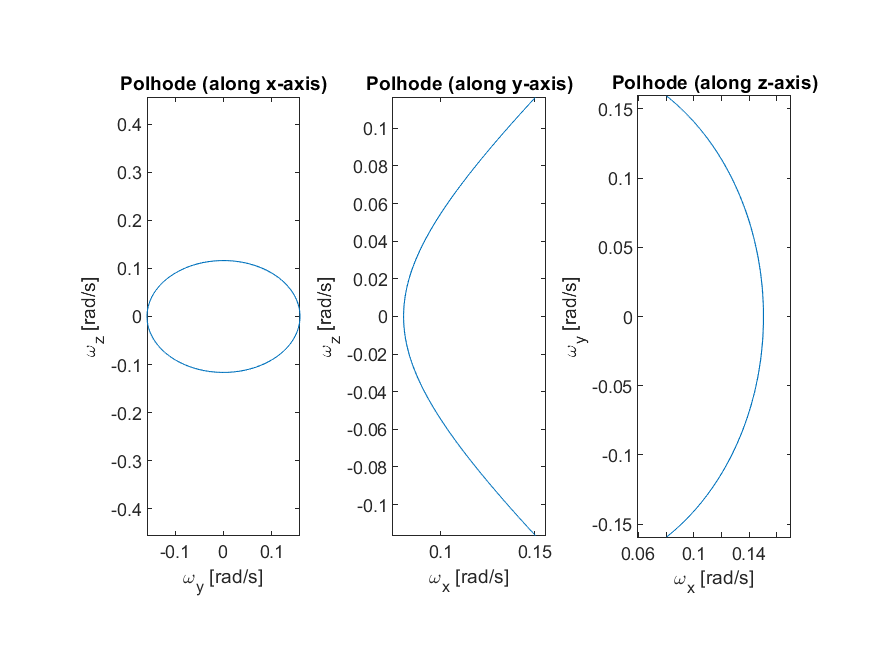
\includegraphics[scale=0.7]{Images/ps2_problem8.png}
\caption{2D views of polhode}
\label{fig:ps2_problem8}
\end{figure}


\subsection{PROBLEM 9}
\textit{Repeat above steps changing initial conditions, e.g. setting angular velocity vector parallel to principal axis. Is the behavior according to expectations?}

We show the angular velocity evolution with the initial conditions shown in Table \ref{tab:ps2_problem9_conditions}. Case 1 involves rotation about the principal x-axis, Case 2 involves rotation about the principal y-axis with a slight disturbance, and Case 3 involved rotation about the z-axis with a slight disturbance.

\begin{table}[H]
\centering
\label{tab:ps2_problem9_conditions}
\begin{tabular}{|l|l|l|l|}
\hline
\textbf{Case} & \textbf{$\omega_x$ (deg/s)} & \textbf{$\omega_y$ (deg/s)} & \textbf{$\omega_z$ (deg/s)} \\ \hline
1             & 8                     & 0                     & 0                     \\ \hline
2             & 0.08                  & 8                     & 0.08                  \\ \hline
3             & 0.08                  & 0                     & 8                     \\ \hline
\end{tabular}
\end{table}

The specifics of Case 1 are shown in the angular velocity plot in Figure \ref{fig:ps2_problem9_euler_equations_x}, the polhode and ellipsoids in Figure \ref{fig:ps2_problem9_p7_x}, and the 2D views of the polhode in Figure \ref{fig:ps2_problem9_p8_x}. The behavior shown is as expected–when the angular velocity is parallel to the principal axis, we do not have coupling with the other components of angular velocity, and the polhode views in 2D become points rather than conic sections.

For Case 2, Figure \ref{fig:ps2_problem9_euler_equations_y} shows that the satellite's rotational behavior will oscillate as expected, owing to the properties of the intermediate axis. Additionally, Figure \ref{fig:ps2_problem9_p7_y}, and the 2D views in Figure \ref{fig:ps2_problem9_p8_y} show a larger polhode, with the slight disturbances leading to ellipsoids with a substantial intersection. Interestingly, there seems to be a very sharp hyperbola in the xz-plane of the polhode.

Figure \ref{fig:ps2_problem9_euler_equations_z} illustrates a slight oscillation of angular velocities about the x- and y-axes in Case 3. Meanwhile, the actual region of intersection in the polhode as shown in Figures \ref{fig:ps2_problem9_p7_z} and \ref{fig:ps2_problem9_p8_z} is much smaller than in other cases, but not a single point like in the Case 1.

\begin{figure}[H]
\centering
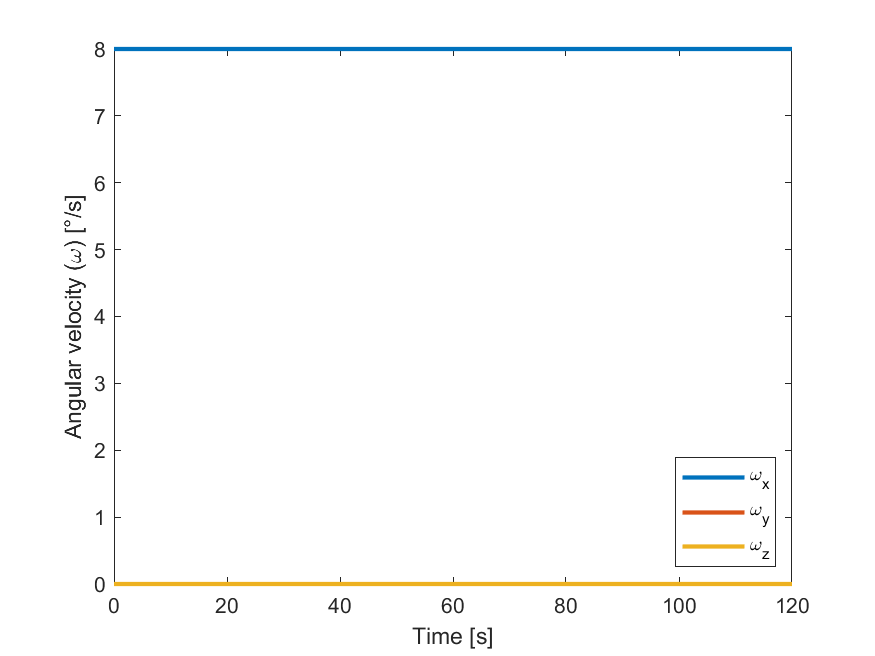
\includegraphics[scale=0.6]{Images/ps2_problem9_euler_equations_x.png}
\caption{Angular velocity evolution for angular velocity vector for Case 1}
\label{fig:ps2_problem9_euler_equations_x}
\end{figure}

\begin{figure}[H]
\centering
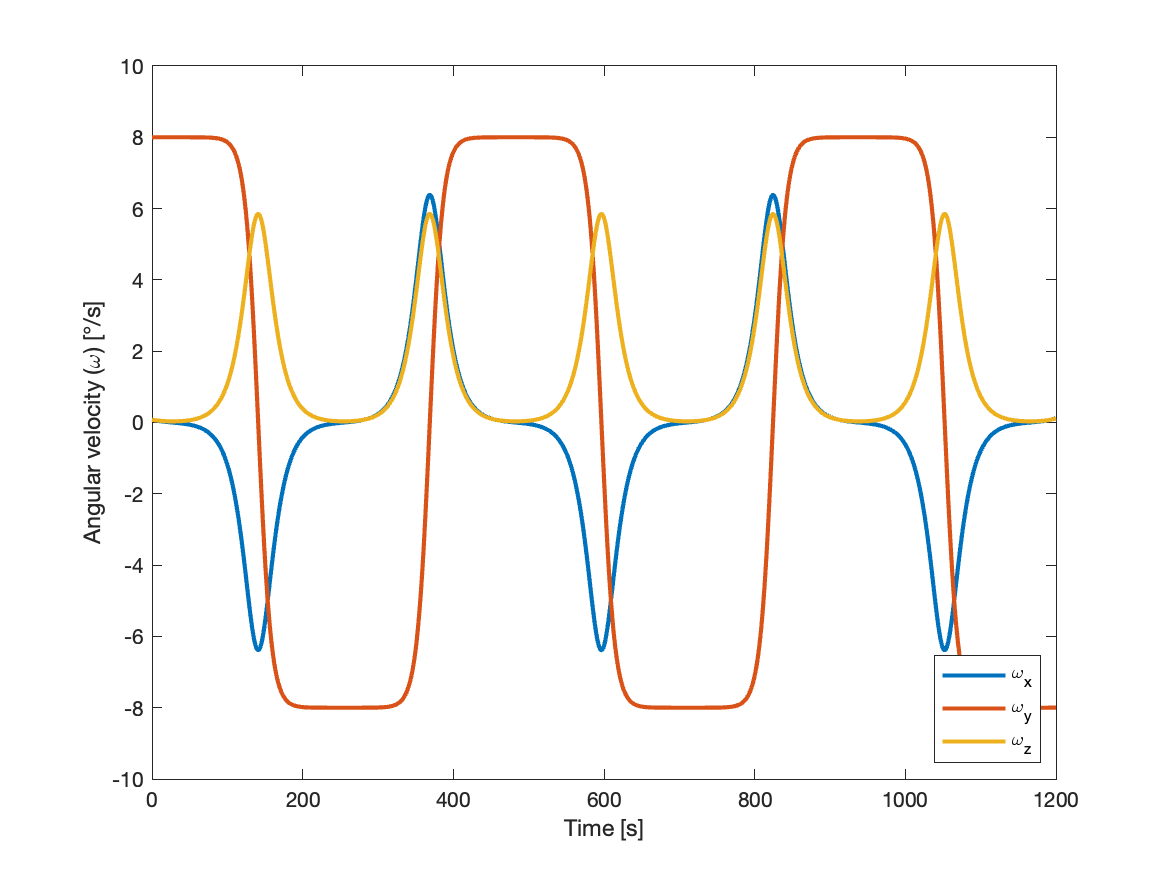
\includegraphics[scale=0.6]{Images/ps2_problem9_euler_equations_y.png}
\caption{Angular velocity evolution for angular velocity vector for Case 2}
\label{fig:ps2_problem9_euler_equations_y}
\end{figure}

\begin{figure}[H]
\centering
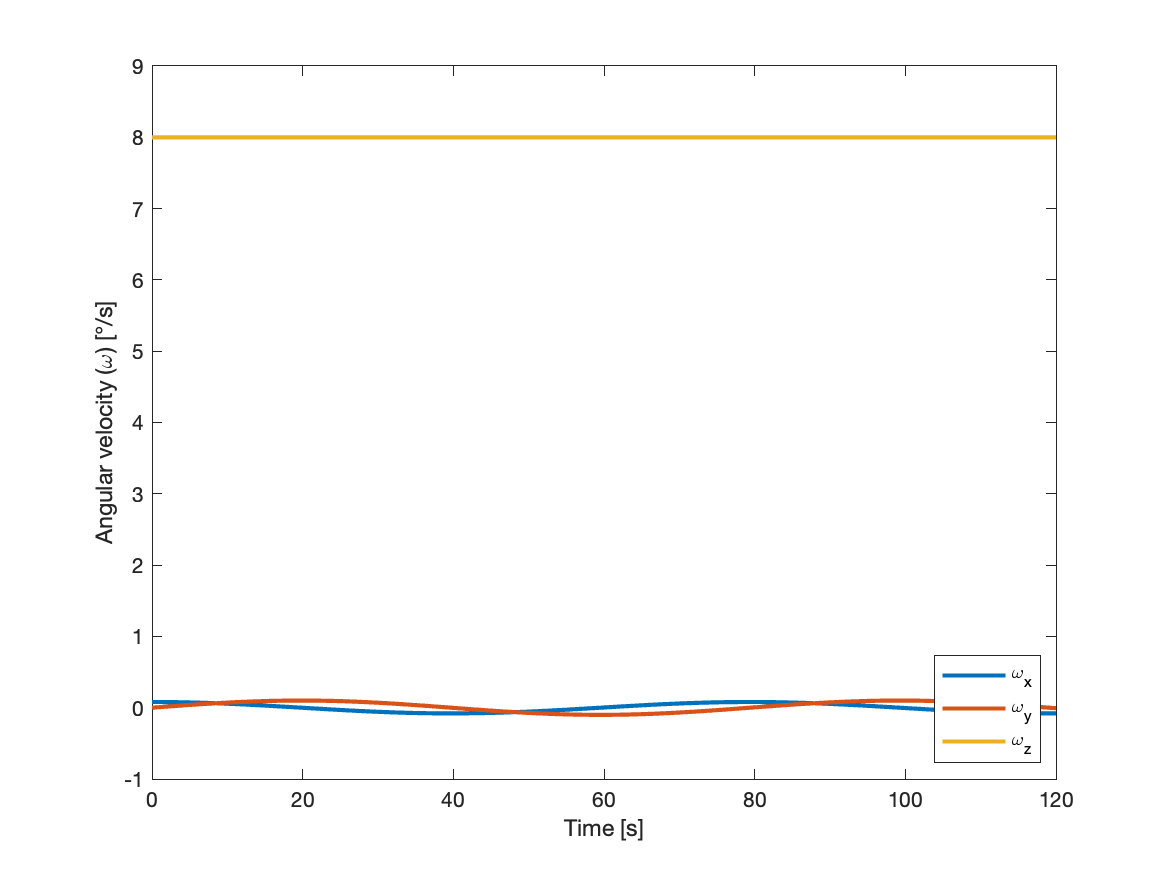
\includegraphics[scale=0.6]{Images/ps2_problem9_euler_equations_z.png}
\caption{Angular velocity evolution for angular velocity vector for Case 3}
\label{fig:ps2_problem9_euler_equations_z}
\end{figure}

\begin{figure}[H]
\centering
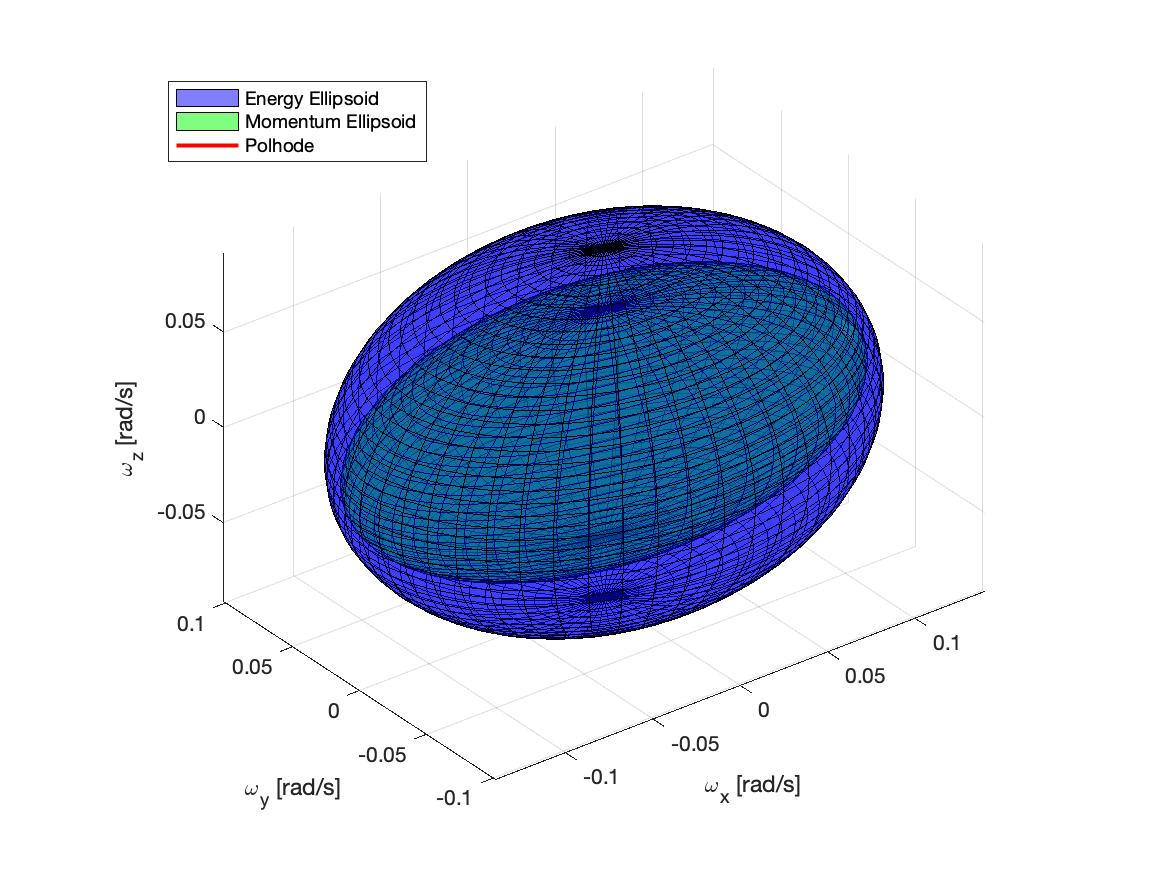
\includegraphics[scale=0.6]{Images/ps2_problem9_p7_x.png}
\caption{Polhode and ellipsoids for angular velocity vector for Case 1}
\label{fig:ps2_problem9_p7_x}
\end{figure}

\begin{figure}[H]
\centering
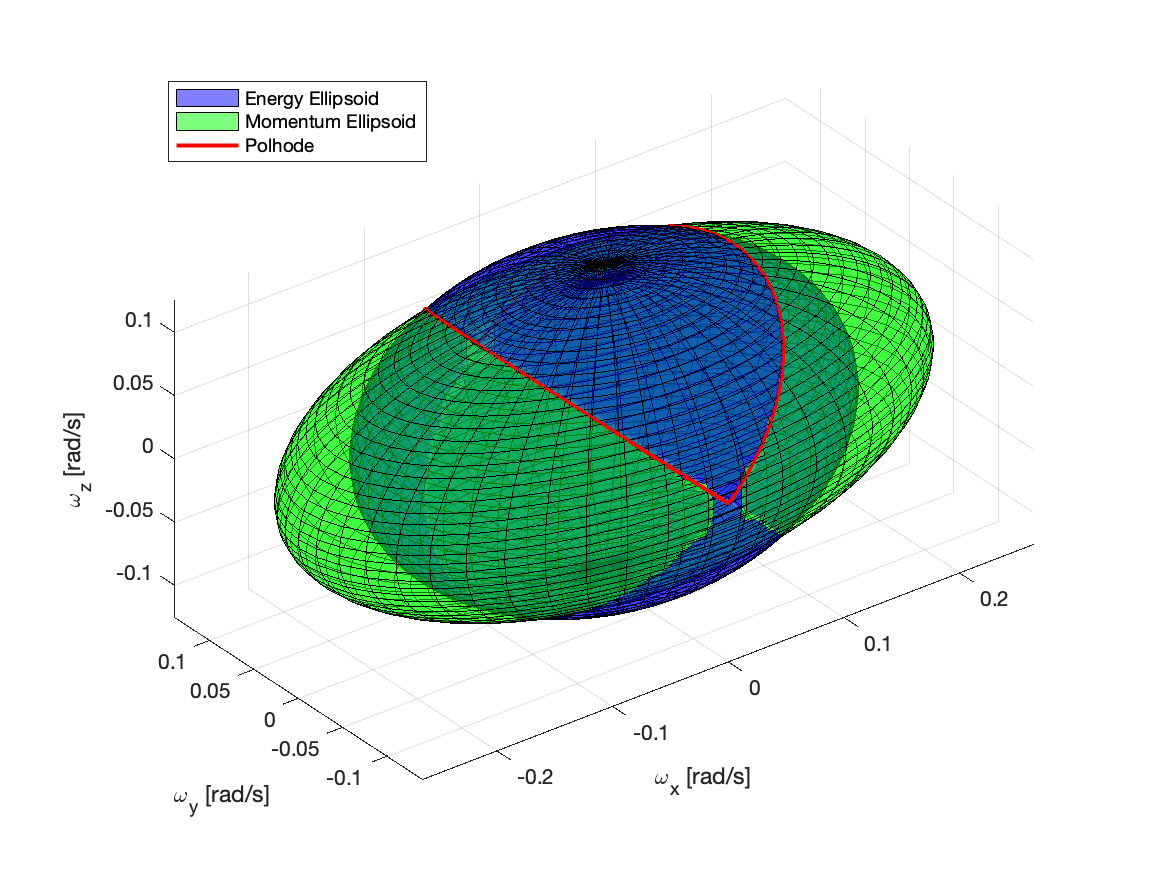
\includegraphics[scale=0.6]{Images/ps2_problem9_p7_y.png}
\caption{Polhode and ellipsoids for angular velocity vector for Case 2}
\label{fig:ps2_problem9_p7_y}
\end{figure}

\begin{figure}[H]
\centering
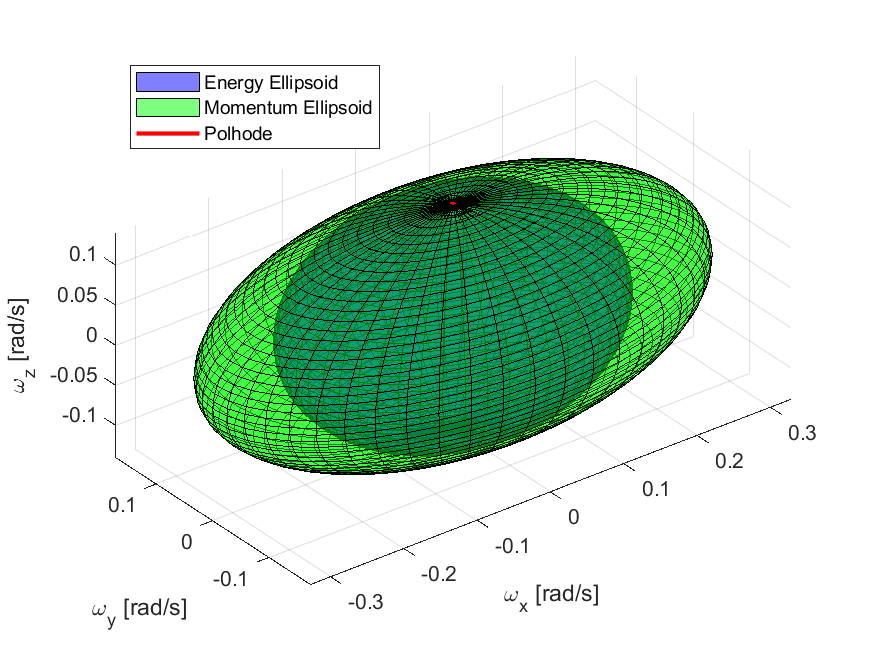
\includegraphics[scale=0.6]{Images/ps2_problem9_p7_z.png}
\caption{Polhode and ellipsoids for angular velocity vector for Case 3}
\label{fig:ps2_problem9_p7_z}
\end{figure}

\begin{figure}[H]
\centering
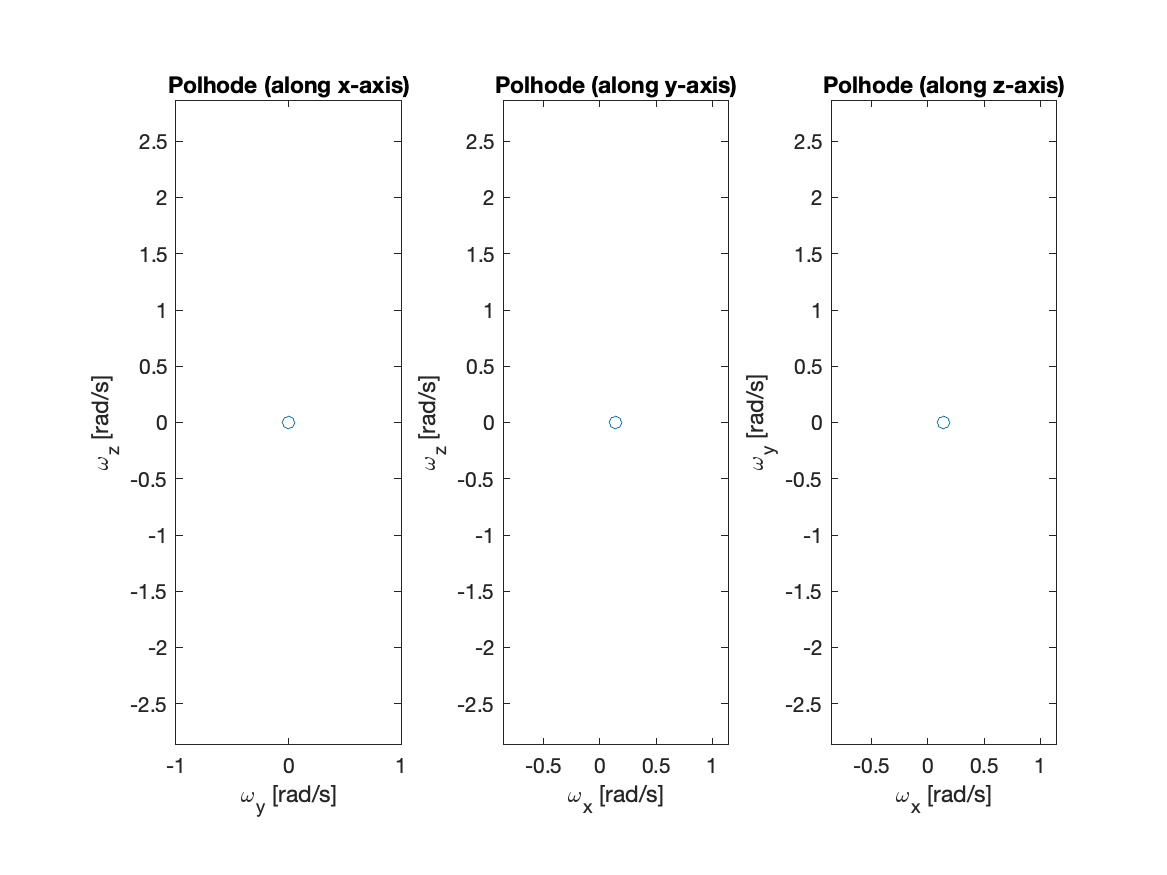
\includegraphics[scale=0.6]{Images/ps2_problem9_p8_x.png}
\caption{2D views of polhode for angular velocity vector for Case 1}
\label{fig:ps2_problem9_p8_x}
\end{figure}

\begin{figure}[H]
\centering
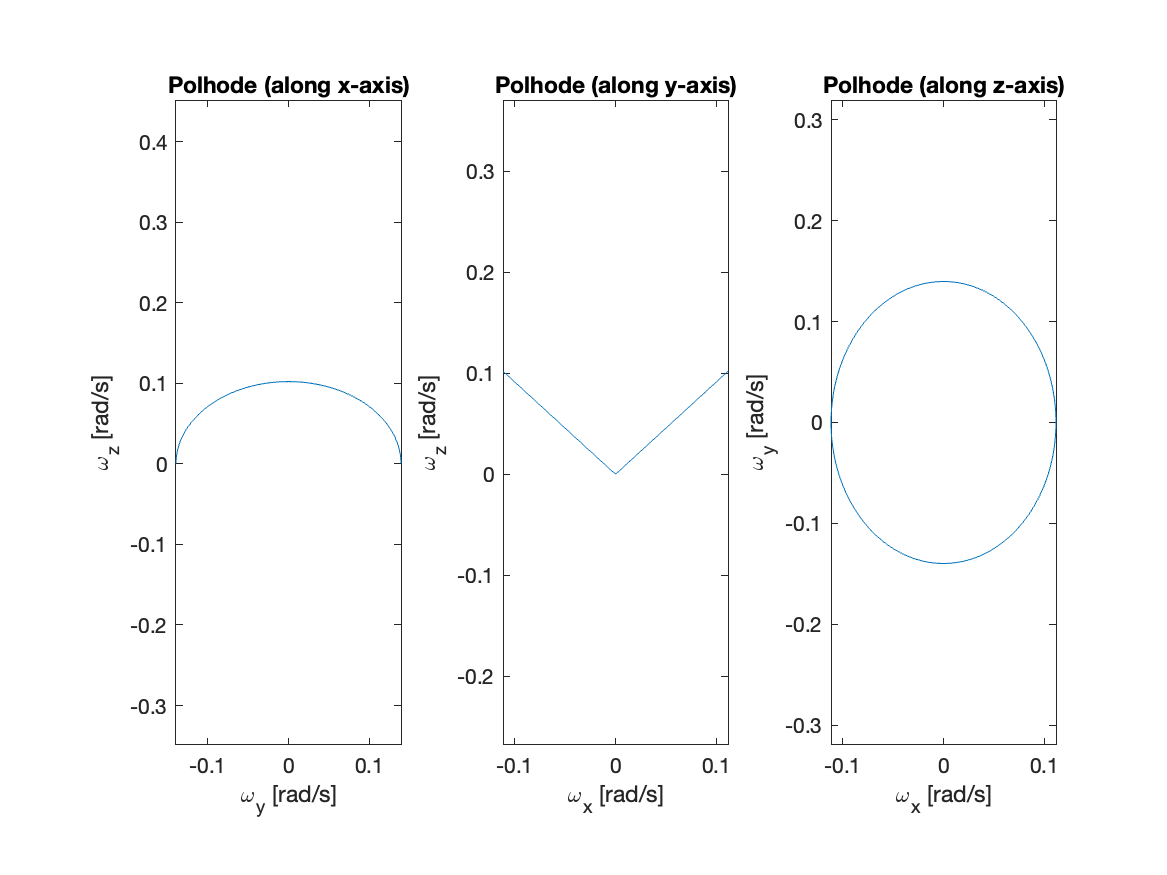
\includegraphics[scale=0.6]{Images/ps2_problem9_p8_y.png}
\caption{2D views of polhode for angular velocity vector for Case 2}
\label{fig:ps2_problem9_p8_y}
\end{figure}

\begin{figure}[H]
\centering
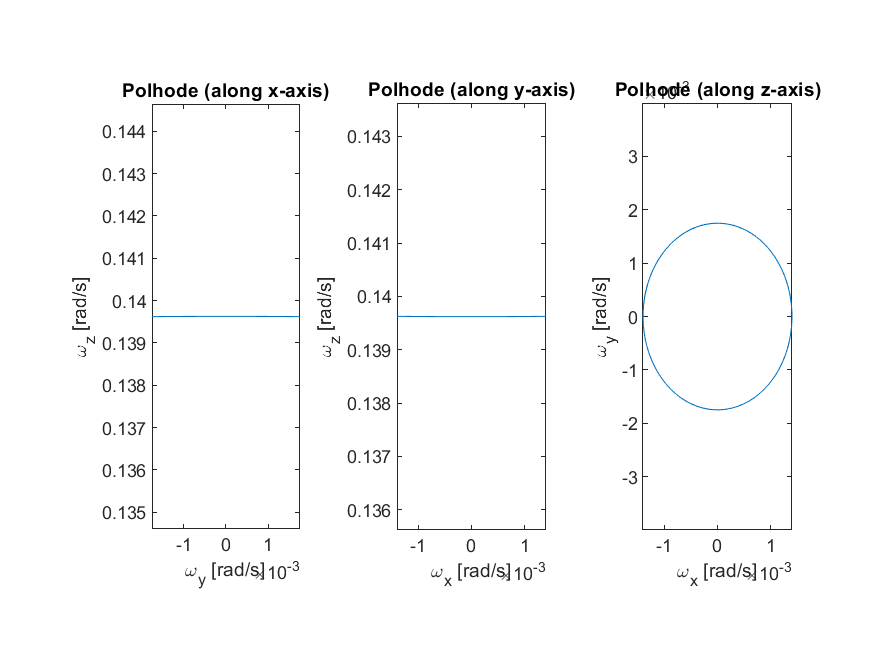
\includegraphics[scale=0.6]{Images/ps2_problem9_p8_z.png}
\caption{2D views of polhode for angular velocity vector for Case 3}
\label{fig:ps2_problem9_p8_z}
\end{figure}

% \section{\Large PROBLEM SET 3}
\subsection{PROBLEM 1}
\textit{Impose that satellite is axial-symmetric (Ix$=$Iy$\neq$Iz). Repeat numerical simulation from previous pset using initial condition 4) from previous pset.}


\subsection{PROBLEM 2}
\textit{Program analytical solution for axial-symmetric satellite. Compute it at same time steps and from same initial conditions.}


\subsection{PROBLEM 3}
\textit{Compare numerical and analytical solutions. Plot differences (errors), do not only superimpose absolute values. Tune numerical integrator for large discrepancies. Are angular velocity vector and angular momentum vector changing according to theory in principal axes?}


\subsection{PROBLEM 4}
\textit{Program Kinematic equations of motion correspondent to a nominal attitude parameterization of your choice.}


\subsection{PROBLEM 5}
\textit{Program Kinematic equations of motion correspondent to a different attitude parameterization from the previous step. This is used for comparison, to get familiar with different approaches, and as fall back solution in the case of singularities.}


\subsection{PROBLEM 6}
\textit{Numerically integrate Euler AND Kinematic equations from arbitrary initial conditions (warning: stay far from singularity of adopted parameterization). Multiple revolutions. The output is the evolution of the attitude parameters over time. These attitude parameters describe orientation of principal axes relative to inertial axes.}


\subsection{PROBLEM 7}
\textit{ISince inertial position, velocity, and attitude, are known at the same time throughout the simulation, it is now possible to express vectors in the reference systems of interest.}



% \section{\Large PROBLEM SET 4}
\subsection{PROBLEM 1}
\textit{Equilibrium tests}

\textit{a. Assume that 2 components of the initial angular velocities are zero and that the principal axes are aligned with the inertial frame (e.g., zero Euler angles). Verify that during the simulation the 2 components of angular velocity remain zero and that the attitude represents a pure rotation about the rotation axis (e.g., linearly increasing Euler angle). Plot velocities and angles.}

For this problem, we assumed that the initial angular velocity and Euler angles were what is shown below. The initial Euler angles were not initialized to be all 0 because we used 3-1-3 Euler angle representation, meaning that Euler angles at 0 would lead to a singularity. While this work-around is not ideal in the situation that the satellite operates around zero Euler angles, for the sake of this exercise this should be adequate.
\begin{align*}
\Vec{\omega} &= 
\qty[parse-numbers = false]{
    \begin{bmatrix}
    0 \\
    0 \\
    1 \\ 
    \end{bmatrix}
}{\radian\per\s}
\end{align*}
\begin{align*}
\phi = \qty[parse-numbers = false]{0}{\radian}, \;\;\;
\theta = \qty[parse-numbers = false]{1e-9}{\radian}, \;\;\;
\psi = \qty[parse-numbers = false]{0}{\radian}
\end{align*}

As can be seen in Figure \ref{fig:ps4_problem1a_velocity}, $\omega_x$ and $\omega_y$ remained 0, while $\omega_z$ was a constant value, as expected. Similarly, in Figure \ref{fig:ps4_problem1a_angle} the $\phi$ and $\theta$ Euler angles stayed zero while the $\psi$ Euler angle varied. 

\begin{figure}[H]
\centering
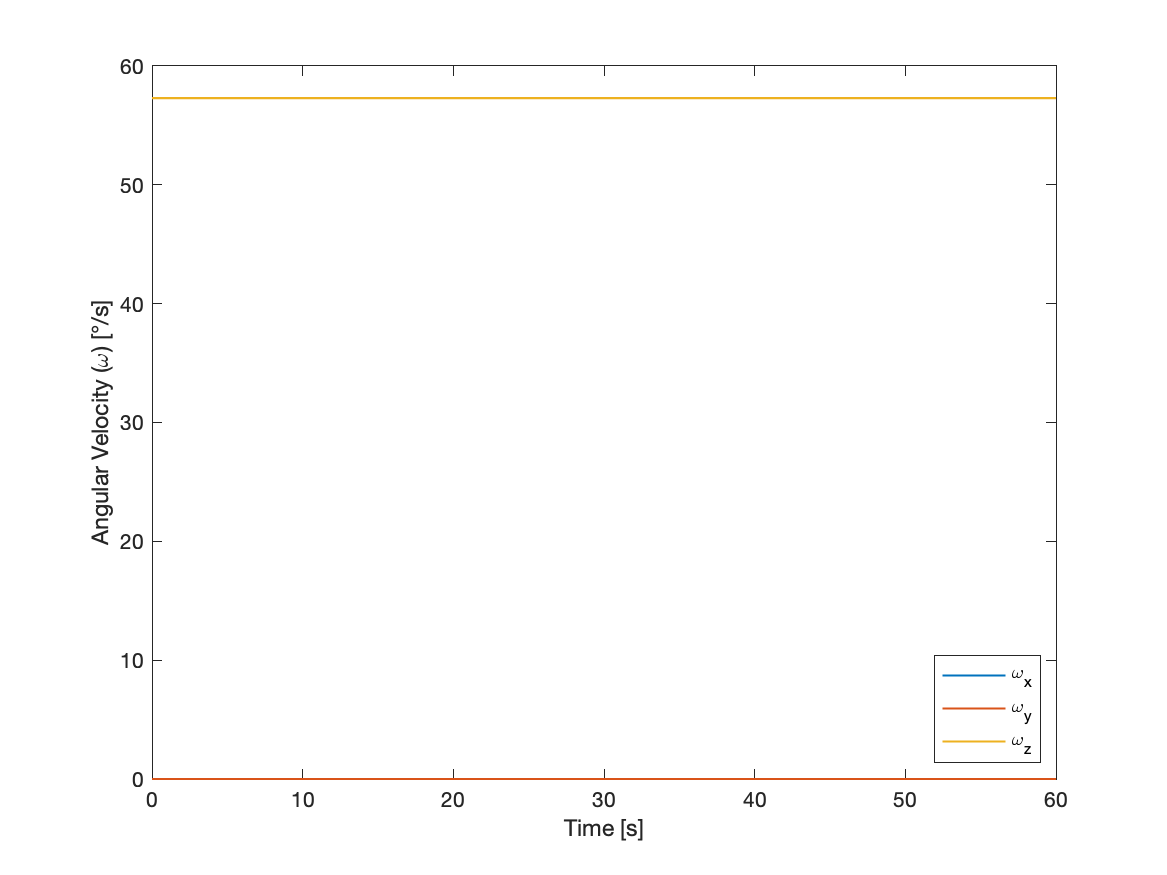
\includegraphics[scale=0.6]{Images/ps4_problem1a_angvel.png}
\caption{Evolution of angular velocity}
\label{fig:ps4_problem1a_angvel}
\end{figure}

\begin{figure}[H]
\centering
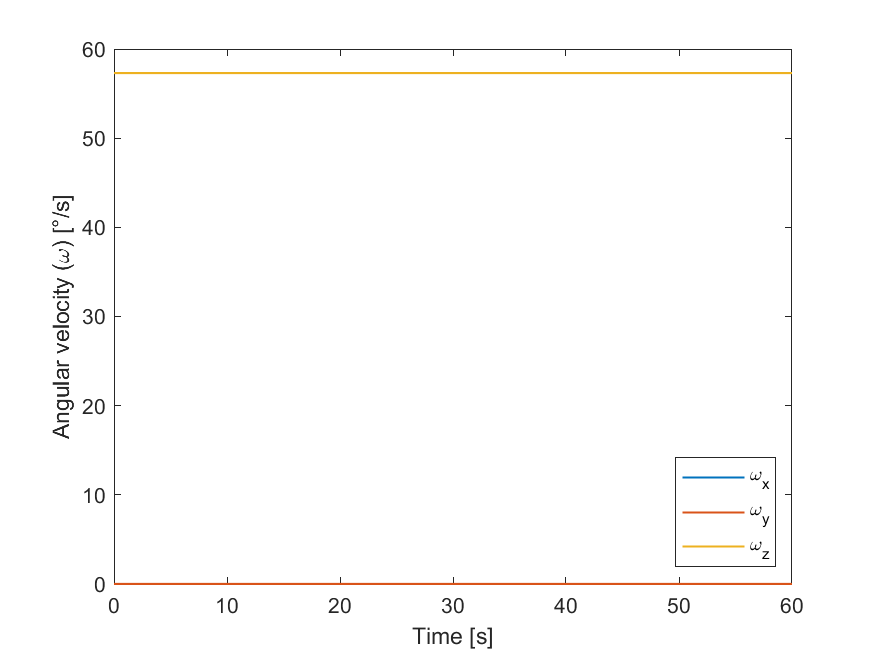
\includegraphics[scale=0.6]{Images/ps4_problem1a_angle.png}
\caption{Evolution of Euler angles}
\label{fig:ps4_problem1a_angle}
\end{figure}

\textit{b. Repeat a. by setting the initial attitude to match the RTN frame. Set the initial angular velocity to be non-zero only about N. Show the evolution of attitude motion in the RTN frame and give an interpretation of the results (recall that you might have J2 effects in orbit propagation, consider removing them for verification).}

In the event that initial angular velocity is along only the normal, the angular velocity remains constant throughout the orbit, as seen in Figure \ref{fig:ps4_problem1b_angvel}. From Figure \ref{fig:ps4_problem1b_euler}, we see that the $\theta$ and $\psi$ Euler angles are constant while $\phi$ varies.

\begin{figure}[H]
\centering
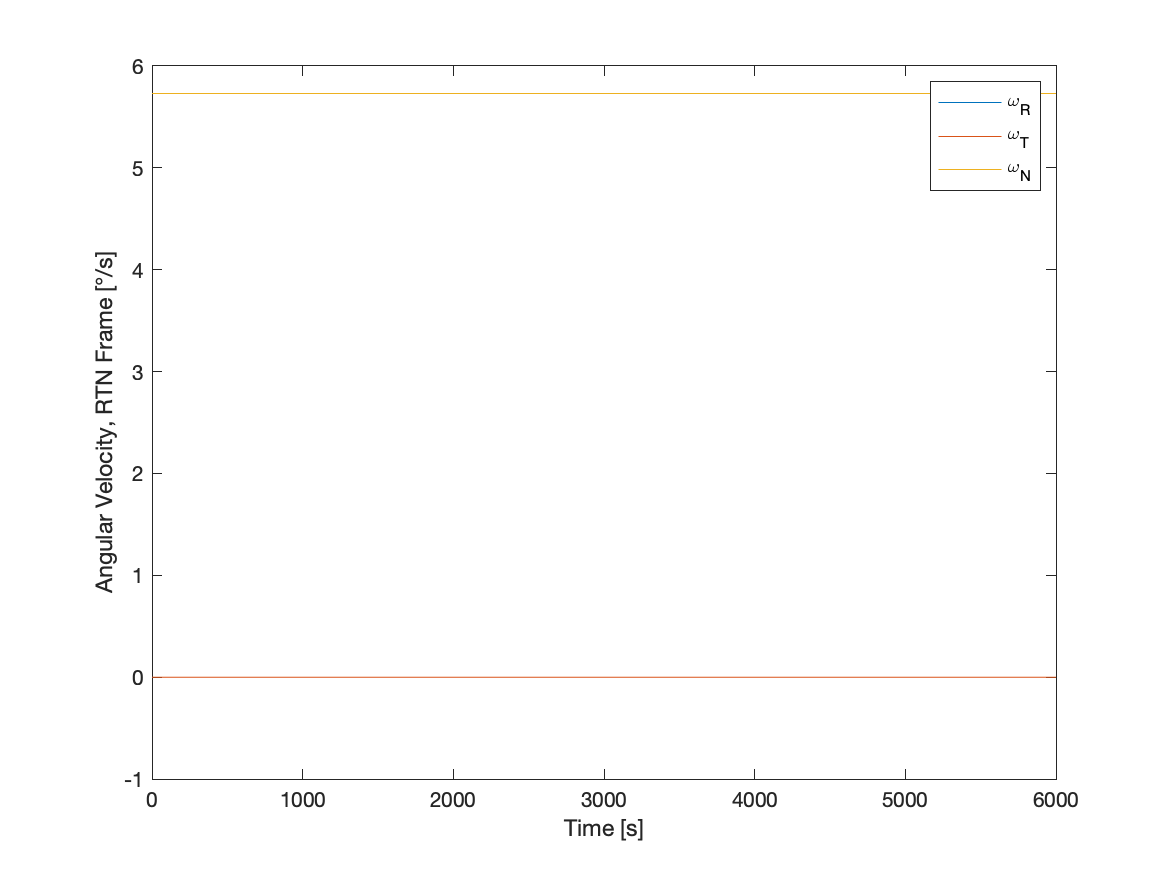
\includegraphics[scale=0.6]{Images/ps4_problem1b_angvel.png}
\caption{Evolution of angular velocity}
\label{fig:ps4_problem1b_angvel}
\end{figure}

\begin{figure}[H]
\centering
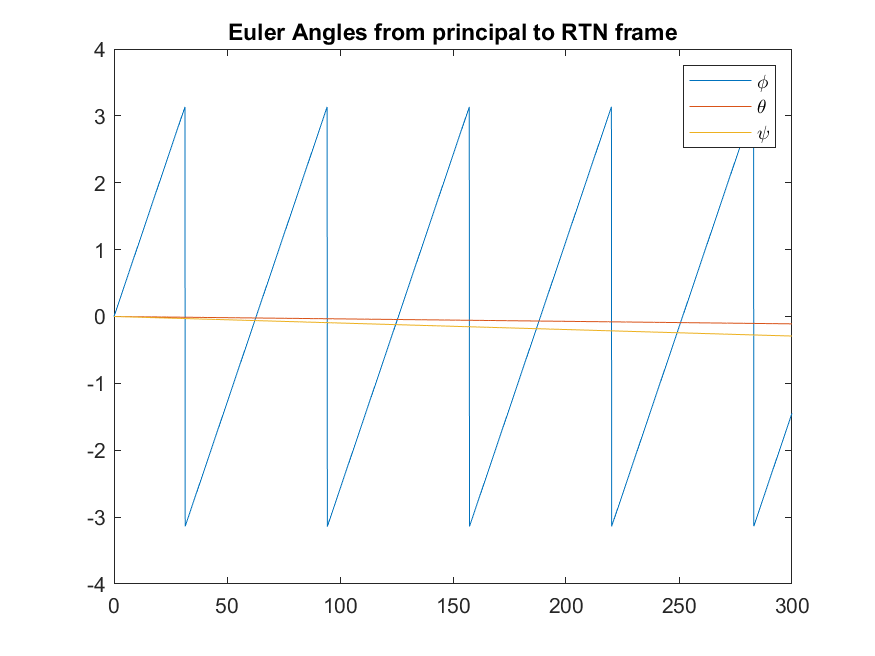
\includegraphics[scale=0.6]{Images/ps4_problem1b_euler.png}
\caption{Evolution of Euler angles}
\label{fig:ps4_problem1b_euler}
\end{figure}


\subsection{PROBLEM 2}
\textit{Stability tests}

\textit{a. Pretend you have a single-spin satellite. Set initial conditions to correspond alternatively to the 3 possible equilibrium configurations (rotation about principal axes of inertia). Slightly perturb initial condition. Is the attitude stable or unstable? In angles and velocities? If stable, periodically or asymptotically? Show it.}

For a single spin satellite, the three possible equilibrium configurations are spinning on its minimum principal axis, spinning on its intermediate principal axis, and spinning on its
maximum principal axis. Figures \ref{fig:ps4_problem2a_1}, \ref{fig:ps4_problem2a_2}, \ref{fig:ps4_problem2a_3}, all show that the Euler angles are relatively unstable in for the intermediate and minimum axes, and is much more stable along the maximum axis. However, the angular velocities are periodically stable when spinning along the minimum and maximum axes and unstable when spinning on the intermediate axis.

\begin{figure}[H]
\centering
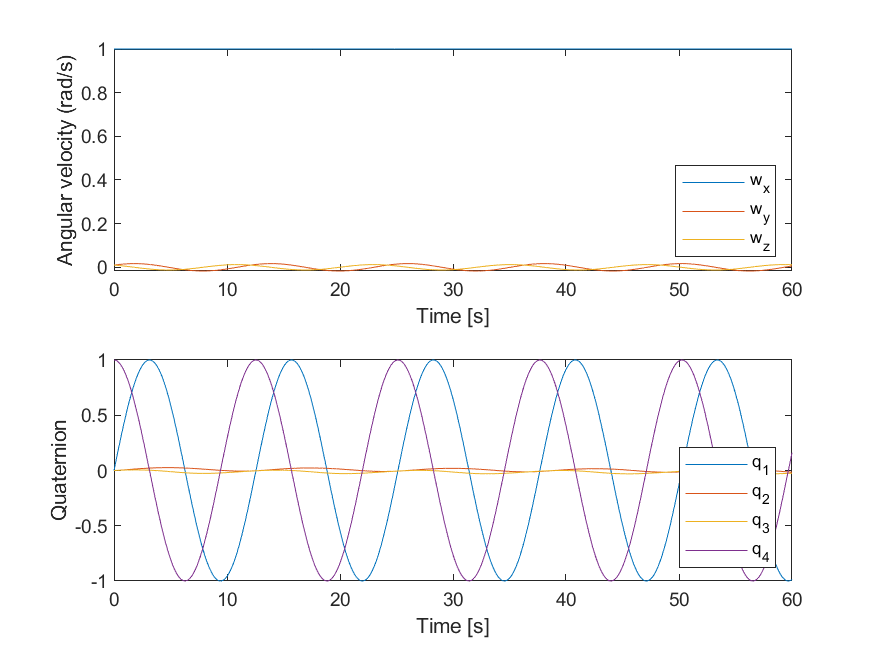
\includegraphics[scale=0.6]{Images/ps4_problem2a_1.png}
\caption{Simulation of satellite spinning on its minimum principal axis}
\label{fig:ps4_problem2a_1}
\end{figure}

\begin{figure}[H]
\centering
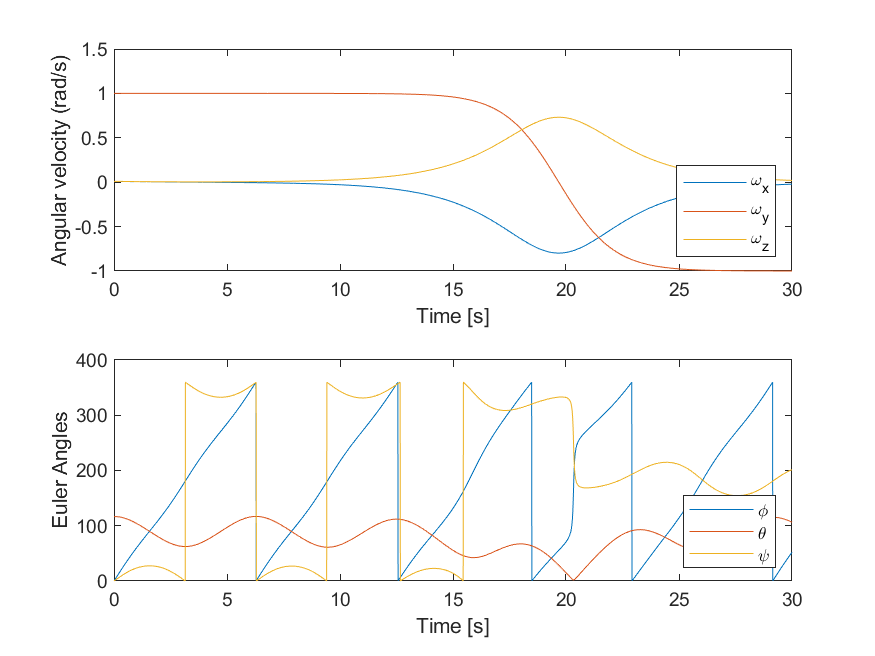
\includegraphics[scale=0.6]{Images/ps4_problem2a_2.png}
\caption{Simulation of satellite spinning on its intermediate principal axis}
\label{fig:ps4_problem2a_2}
\end{figure}

\begin{figure}[H]
\centering
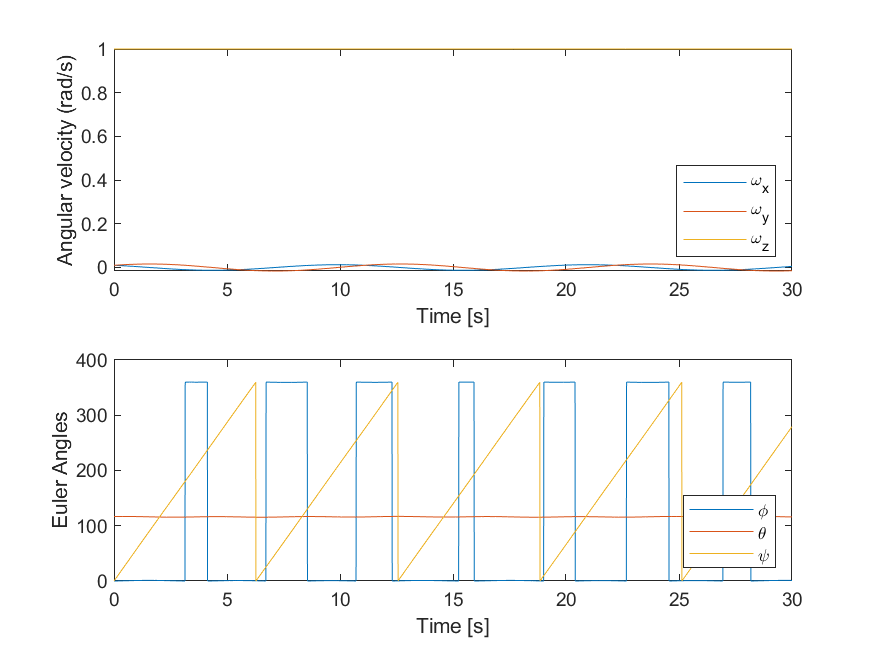
\includegraphics[scale=0.6]{Images/ps4_problem2a_3.png}
\caption{Simulation of satellite spinning on its maximum principal axis}
\label{fig:ps4_problem2a_3}
\end{figure}

\subsection{PROBLEM 3}
\textit{Adding a momentum wheel or rotor (dual-spin satellite)}

\textit{a. Re-program Euler equations to include a generic momentum wheel or rotor with rotation axis aligned with one of the principal axes of inertia. Ideally the wheel or rotor has specs representative of commercial products (inertia, rotational speed).}

The equations that implement the generic momentum wheel with the rotor into the Euler equations are below.

\begin{align*}
    I_x \dot{\omega_x} + I_r \dot{\omega_r} r_x + (I_z - I_y) \omega_y \omega_z 
    + I_r \omega_r (\omega_y r_z - \omega_z r_y) = M_x \\
    I_y \dot{\omega_y} + I_r \dot{\omega_r} r_y + (I_x - I_z) \omega_z \omega_x 
    + I_r \omega_r (\omega_z r_x - \omega_x r_z) = M_y \\
    I_z \dot{\omega_z} + I_r \dot{\omega_r} r_z + (I_y - I_x) \omega_x \omega_y 
    + I_r \omega_r (\omega_x r_y - \omega_y r_x) = M_z \\
    I_r \dot{\omega_r} = M_r
\end{align*}

The function kinEulerAngleWheel was used in addition to ode113 to simulate the angular velocities over time.

\textit{b. Numerically integrate Euler AND Kinematic equations from equilibrium initial condition. Verify that integration is correct as from previous tests (conservation laws, rotations, etc.).}

kinEulerAngleWheel was modified to also account for the kinematic equations, as shown before. As we see in Figure \ref{fig:ps4_problem3c_principal}, the overall momentum is conserved in the principal frame, as expected. Additionally, Figure \ref{fig:ps4_problem3c_inertial} shows that the angular momentum vector is conserved in the inertial frame, as expected.

\lstinputlisting{src/kinEulerAngleWheel.m}

\begin{figure}[H]
\centering
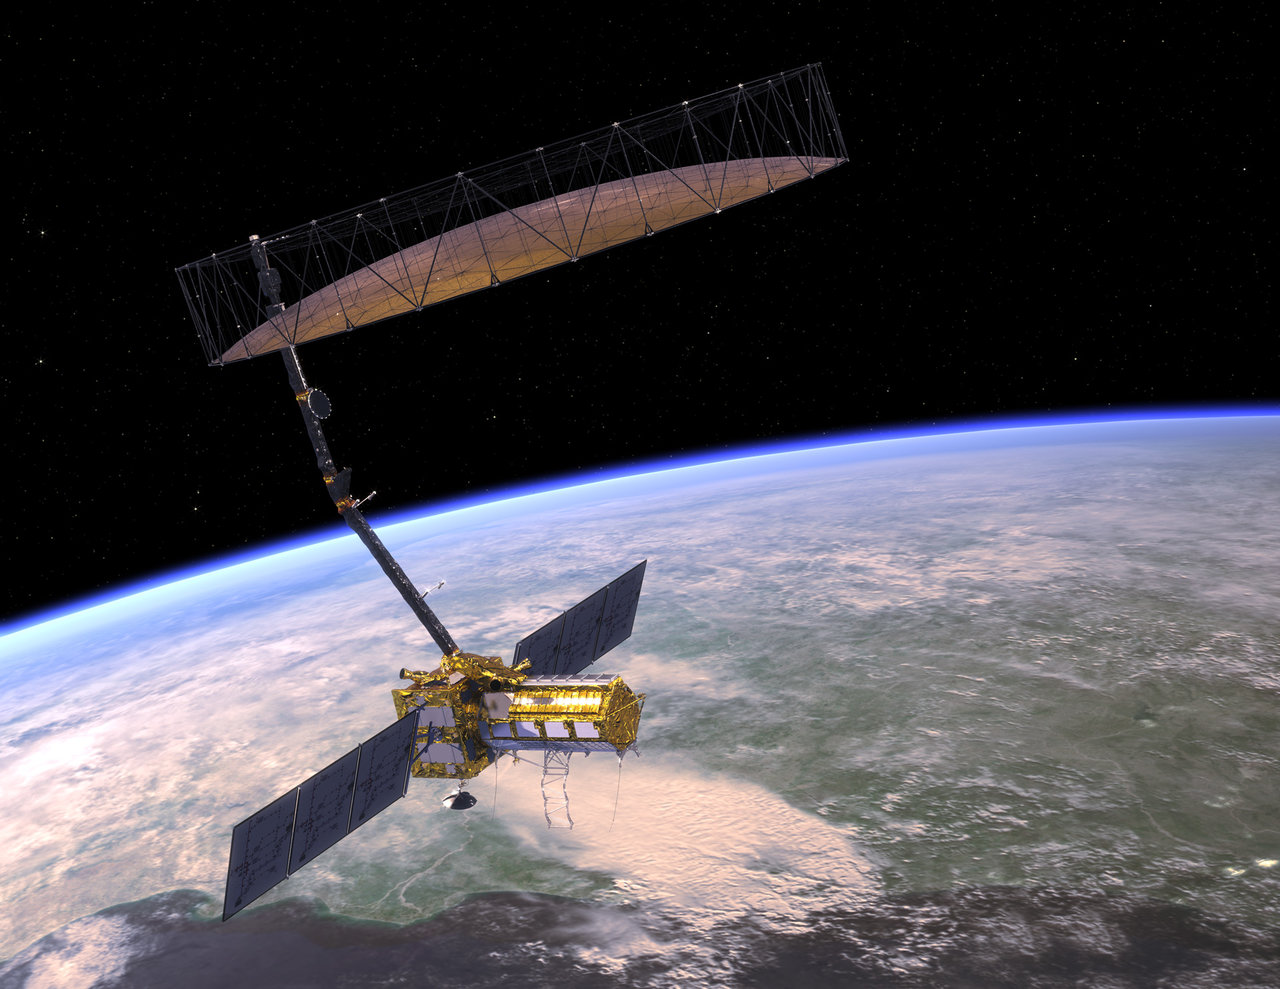
\includegraphics[scale=0.6]{Images/NISAR.jpg}
\caption{Angular Momentum in Principal Frame}
\label{fig:ps4_problem3c_principal}
\end{figure}

\begin{figure}[H]
\centering
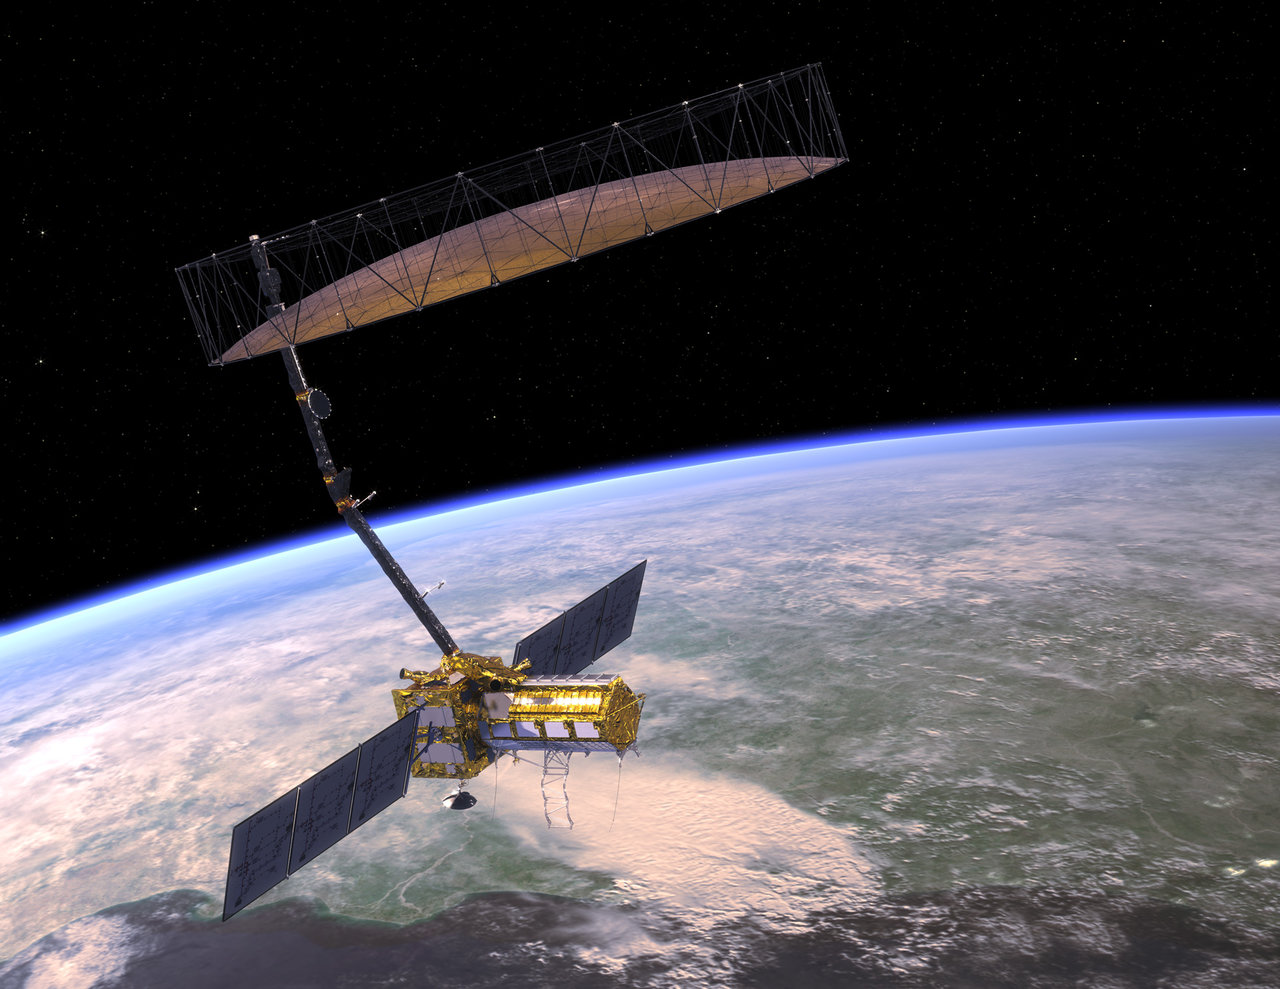
\includegraphics[scale=0.6]{Images/NISAR.jpg}
\caption{Angular Momentum in Inertial Frame}
\label{fig:ps4_problem3c_inertial}
\end{figure}

\textit{c. Verify equilibrium and its stability similar to previous pset.}

Based on linearizing the Euler equations around equilibrium, it can be found that periodic stability can be met with a reaction wheel if one of the following conditions are met:

\begin{align*}
    1)\; I_r \omega_r > (I_y - I_z) \omega_z \;\; AND \;\; I_r \omega_r > (I_x - I_z) \omega_z \\
    2)\; I_r \omega_r < (I_y - I_z) \omega_z \;\; AND \;\; I_r \omega_r < (I_x - I_z) \omega_z \\
\end{align*}

The above equation is specifically for equilibrium about the z-axis, but similar equations hold true for stability about the x and y axes.

Below are the angular velocity plots for stability about the maximum, intermediate, and minimum principal axes.

\textbf{figs}


\textit{d. Use the stability condition to make attitude motion stable for rotation about intermediate moment of inertia by changing moment of inertia and/or angular velocity of the momentum wheel or rotor.}




\textit{e. Try to make rotation about another arbitrary axis (potentially relevant to your project) stable through a generic momentum wheel or rotor.}

\subsection{PROBLEM 4}
\textit{Gravity gradient torque (modeling)}

\textit{a. Remove rotor.}

A new function was created without effect of the rotor.

\textit{b. Program gravity gradient torque. Feed torque to Euler equations. This is the first perturbation you model resulting from the interaction of the spacecraft with the environment. Hint: change your orbit to make gravity gradient significant if that’s not the case.}

The equations for the gravity gradient torque are below.

\begin{align*}
    I_x \dot{\omega_x} + (I_z - I_y) \omega_y \omega_z = 3 n^2 (I_z - I_y) c_y c_z \\
    I_y \dot{\omega_y} + (I_x - I_z) \omega_z \omega_x = 3 n^2 (I_x - I_z) c_z c_x \\
    I_z \dot{\omega_z} + (I_y - I_x) \omega_x \omega_y = 3 n^2 (I_y - I_x) c_x c_y \\
\end{align*}

In the above equation, $\Vec{c} = [cx, cy, cz]$ is the normalized direction of $\Vec{R}$.

The function gravGrad was developed to be used with ode113 to propagate the Euler equations.

\lstinputlisting{src/gravGrad.m}

\textit{c. Verify that the magnitude of the modeled torque is consistent with the orbit and inertia tensor of your satellite. Hint: use simplified formulas from class on modeling of gravity gradient torque.}

The general trends we would expect in the gradient gravity torque is for the value to be zero if the satellite spins on its normal axis at the mean motion and for the magnitude to grow linearly with the inertia tensor. The first property is demonstrated in Figure \textbf{fig1} and the second is demonstrated in Figure \textbf{fig2}.

Additionally, we can estimate the order of magnitude to expect our gravity gradient torques to be based on the below equation.

\begin{align*}
    \Vec{M} &= \frac{3 \mu}{a^3}
    \begin{bmatrix}
    (I_z - I_y) c_y c_z \\
    (I_x - I_z) c_z c_x \\
    (I_y - I_x) c_x c_y
    \end{bmatrix}
\end{align*}

The parameters used were the known moments of inertia ($I_x = \qty{7707}{}$, $I_y = \qty{14563}{}$, $I_z = \qty{18050}{\kilogram\cdot\meter^2}$), known values for Earth ($a = \qty{7125.49}{km}$, $\mu = \qty{398600}{\km^3\per\second^2}$), and an arbitrary $\Vec{c} = [\frac{1}{\sqrt{3}}, \frac{1}{\sqrt{3}}, \frac{1}{\sqrt{3}}]$. With these values, we get:

\begin{align*}
    \Vec{M} &=
\qty[parse-numbers = false]{
    \begin{bmatrix}
    0.384174 \\
    1.13956 \\
    -0.755387
    \end{bmatrix}
    \cdot
    10^{-2}
}{\newton\meter}
\end{align*}

These values are in line with what we see in Figure \textbf{fig}.

\textit{d. Numerically integrate Euler and Kinematic equations including gravity gradient from initial conditions corresponding to body axes aligned with the orbital frame (RTN). Verify that gravity gradient torque is zero, besides numerical errors. Hint: you may need to simplify the orbit to unperturbed circular to achieve this. Check that initial angular velocity matches mean motion.}

The constant gravity gradient was demonstrated in problem 4c in Figure \textbf{same fig as before}. Figure \textbf{fig3} demonstrated that the angular velocity in the normal direction matches the mean motion throughout the orbit.

\textit{e. Numerically integrate Euler and Kinematic equations including gravity gradient from arbitrary initial conditions (e.g., relevant to your project). Plot external torque (3 components w.r.t. time) and resulting attitude motion (depends on attitude parameterization, add Euler angles for better geometrical interpretation) over multiple orbits. Comment on results.}

fuck me with a shoe idk what to put here rn (will add later)

% \section{\Large PROBLEM SET 5}
\subsection{PROBLEM 1}
\textit{Gravity gradient torque (stability)}

\textit{a. Calculate the coefficients Ki of the moments of inertia which drive stability under gravity gradient. Compute and plot regions of stable and unstable motion similar to the picture below:}

The following equations show the relationships for gravity gradient stability in terms of moments of inertia. The first inequality hold for when the pitch is stable, and the last two inequalites hold for when the roll and yaw are stable.

\begin{align*}
    k_N = \frac{I_T - I_R}{I_N}, \;\;\;\;\;
    k_T = \frac{I_N - I_R}{I_T}, \;\;\;\;\;
    k_R = \frac{I_N - I_T}{I_R} \\
    k_T > k_R, \;\;\;\;\;
    k_R k_T > 0, \;\;\;\;\;
    1 + 3 k_T + k_R k_T > 4 \sqrt{k_R k_T}
\end{align*}

We show the plot of stable and unstable motion under gravity gradient. When computing the coefficients using moments of inertia about the principal axes, we obtain the following plot. In this case, we investigate the stability for the satellite when it is rotated such that the spacecraft is oriented appropriately for SAR operations, that is, principal x-axis is anti-radial, principal y-axis is opposite of cross-track, and principal z-axis is opposite of along-track. However, this orientation is unstable, as shown below.

\begin{figure}[H]
\centering
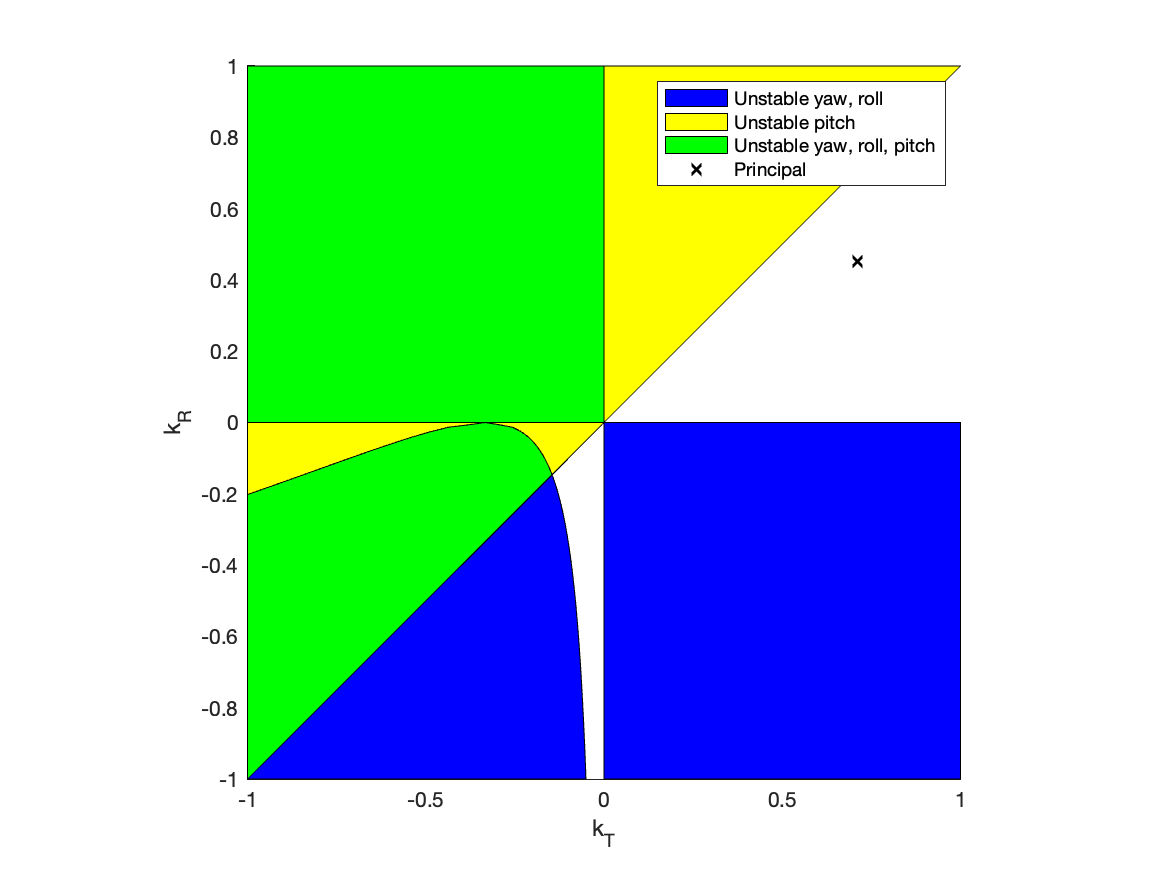
\includegraphics[scale=0.8]{Images/ps5_problem1a.png}
\caption{Stability for nominal axes}
\label{fig:ps5_problem1a}
\end{figure}

\textit{b. Considering the results from 1a, comments on the expected stability of the attitude motion of your satellite about equilibrium. Try to reproduce stable and unstable motion by setting proper initial conditions and perturbing those conditions slightly (e.g., by 1\%). Plot attitude parameters (e.g., Euler angles) to show stability or instability.}

First, without perturbations, the satellite can maintain steady attitude, demonstrating that this chosen orientation is indeed an equilibrium.

\begin{figure}[H]
\centering
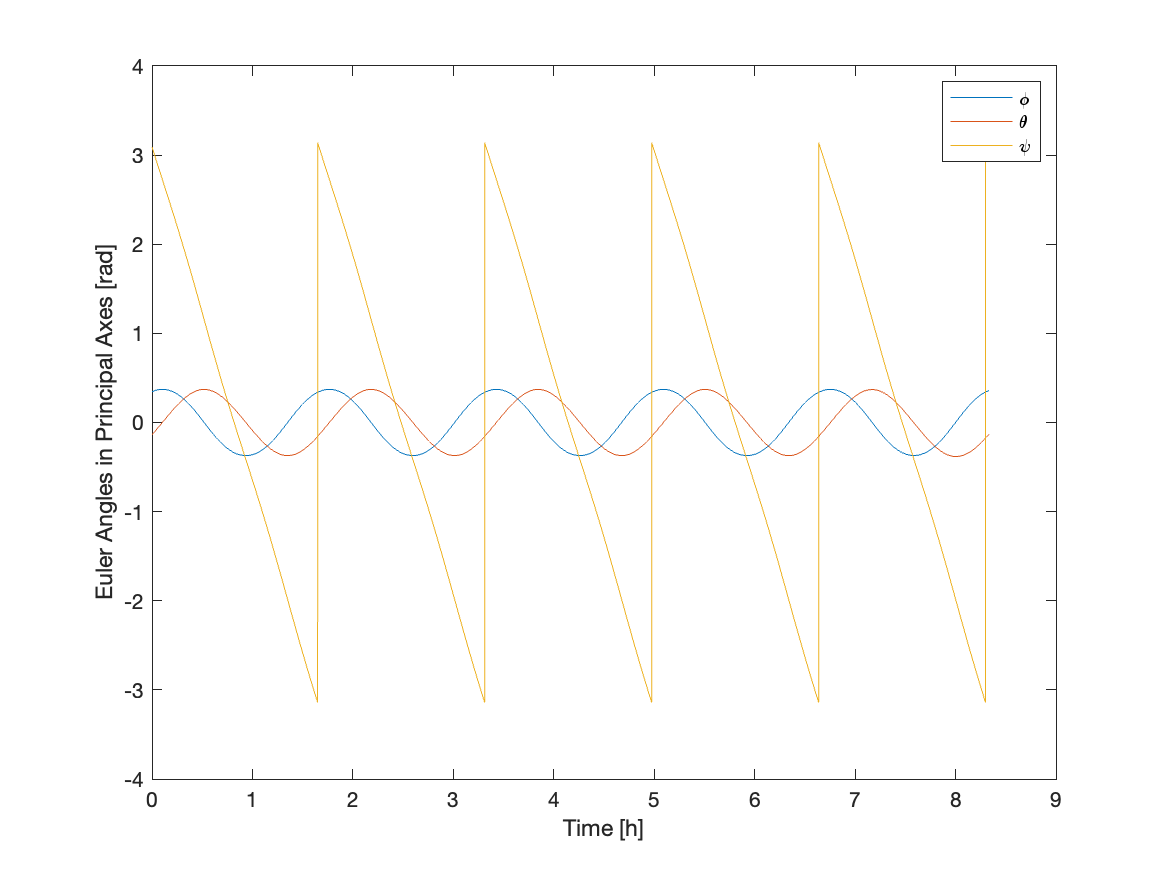
\includegraphics[scale=0.6]{Images/ps5_problem1b_angle_unperturbed.png}
\caption{Attitude evolution for unstable orientation without perturbations}
\label{fig:ps5_problem1b_angle_unperturbed}
\end{figure}

\begin{figure}[H]
\centering
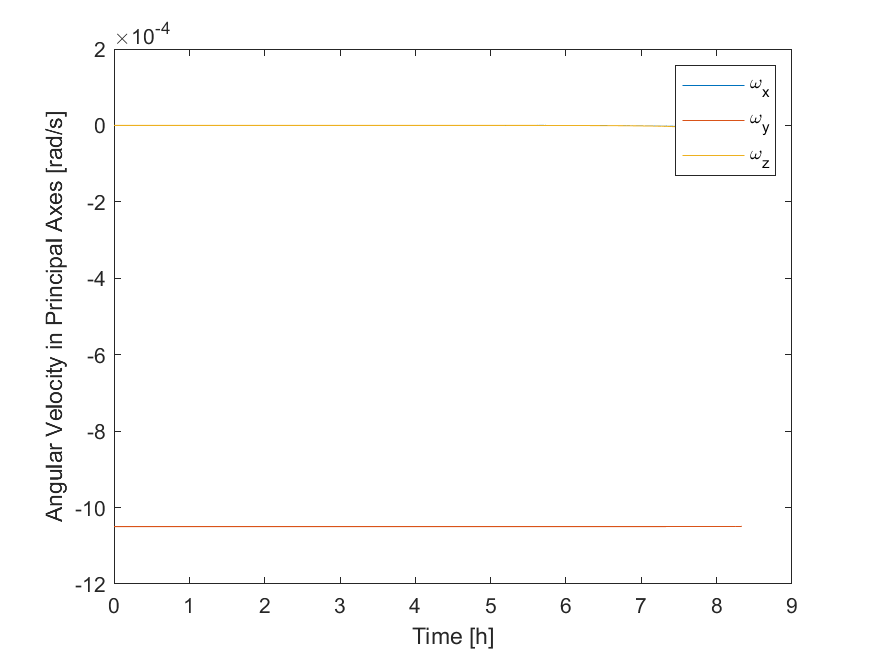
\includegraphics[scale=0.6]{Images/ps5_problem1b_angvel_unperturbed.png}
\caption{Angular velocity evolution for unstable orientation without perturbations}
\label{fig:ps5_problem1b_angvel_unperturbed}
\end{figure}

We expect unstable behavior for small perturbations. Previously, we have already shown that aligning principal axes with RTN produces stable behavior when there are no perturbations. Now, we will introduce small perturbations, causing the system to leave equilibrium and demonstrating that it is unstable.

\begin{figure}[H]
\centering
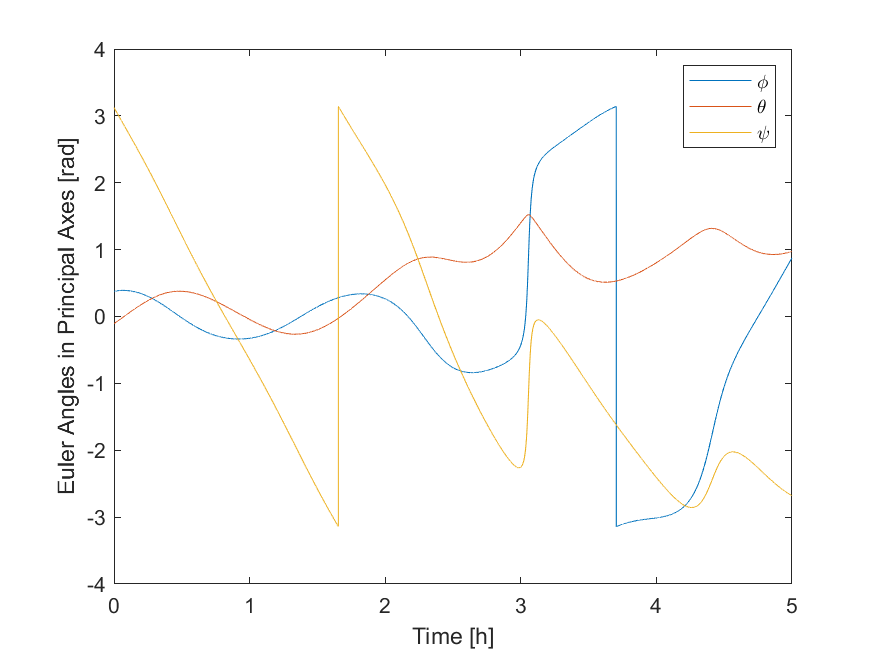
\includegraphics[scale=0.6]{Images/ps5_problem1b_angle.png}
\caption{Attitude evolution for unstable orientation with 1\% perturbations}
\label{fig:ps5_problem1b_angle}
\end{figure}

\begin{figure}[H]
\centering
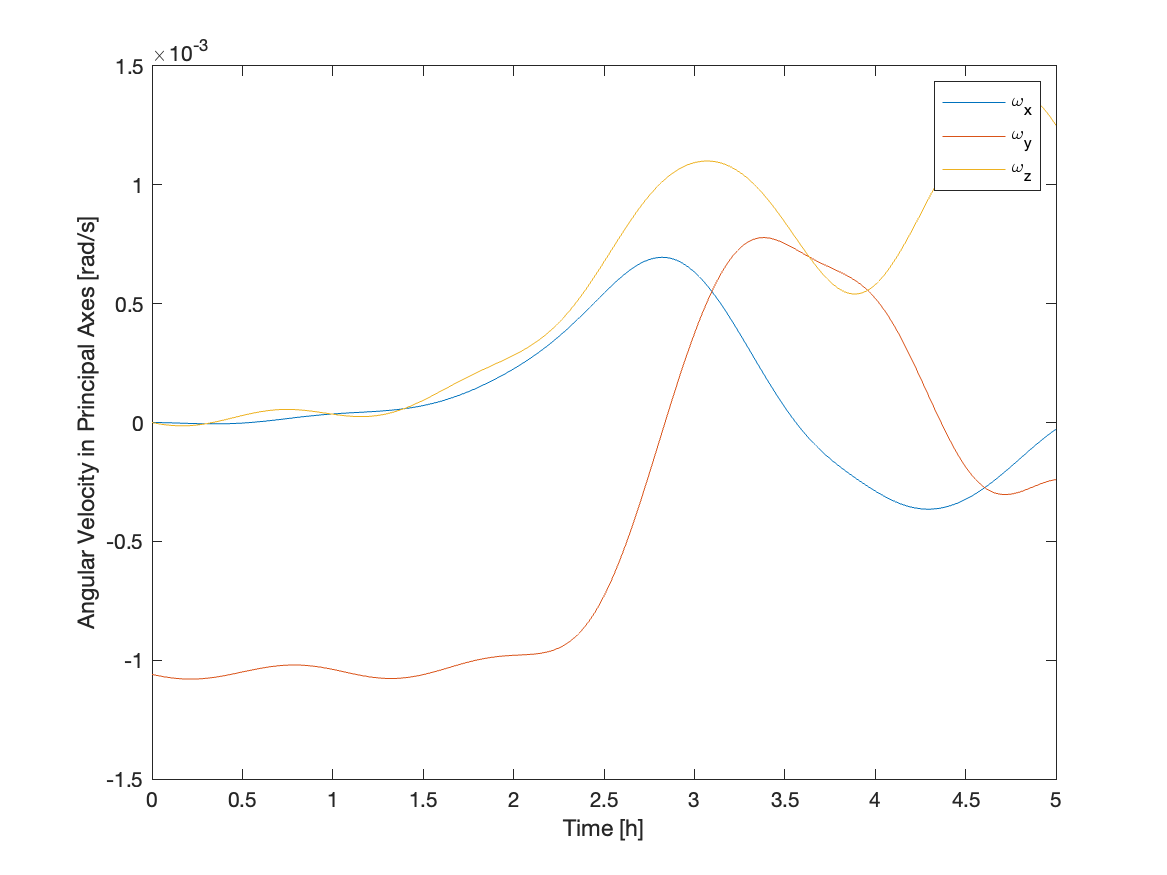
\includegraphics[scale=0.6]{Images/ps5_problem1b_angvel.png}
\caption{Angular velocity evolution for unstable orientation with 1\% perturbations}
\label{fig:ps5_problem1b_angvel}
\end{figure}


\textit{c. How would you need to change the mass distribution and/or nominal attitude of your satellite to obtain stable motion from the gravity gradient torque? Would it make sense for your project? Show a couple of potential configurations in the Ki plane and resulting stability of attitude motion at the equilibrium. This is done by changing your inertia tensor and simulating numerically.}

We will have to align the principal axes XYZ with RTN (respectively) to obtain a stable attitude motion.

\begin{figure}[H]
\centering
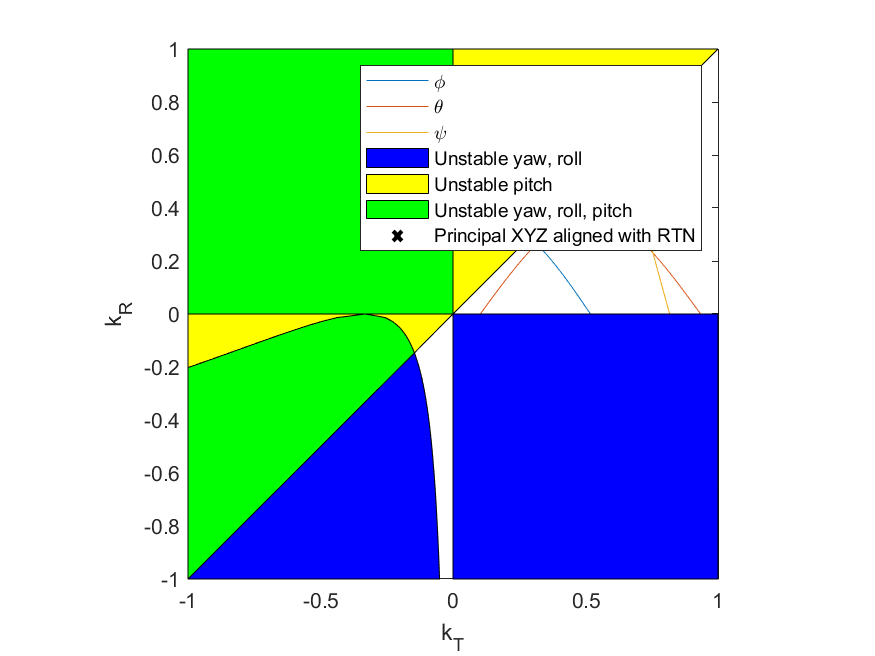
\includegraphics[scale=0.8]{Images/ps5_problem1c.png}
\caption{Stability for aligned principal axes}
\label{fig:ps5_problem1c}
\end{figure}

We expect stable behavior for small perturbations. Previously, we have already shown that aligning principal axes with RTN produces stable behavior when there are no perturbations. Now, we will introduce small perturbations.

\begin{figure}[H]
\centering
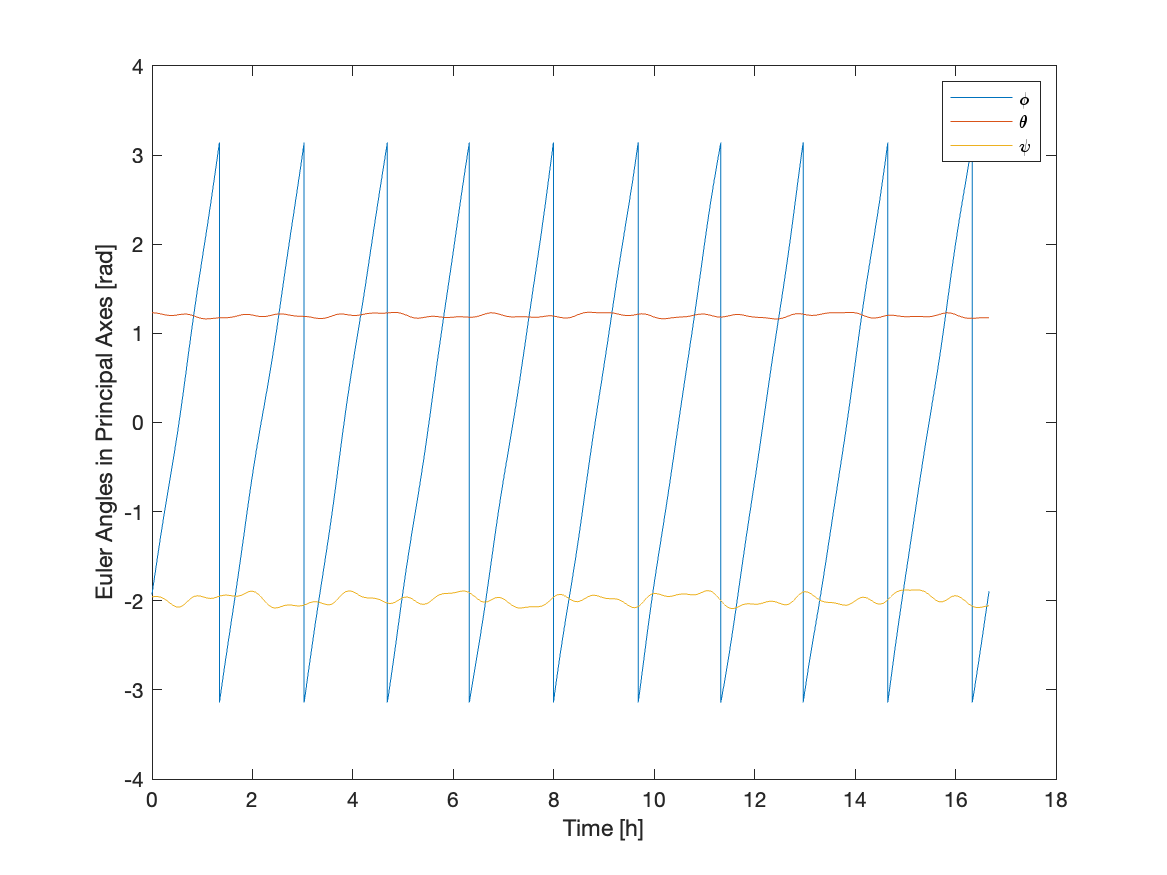
\includegraphics[scale=0.6]{Images/ps5_problem1c_angle.png}
\caption{Attitude evolution for stable orientation with 1\% perturbations}
\label{fig:ps5_problem1c_angle}
\end{figure}

\begin{figure}[H]
\centering
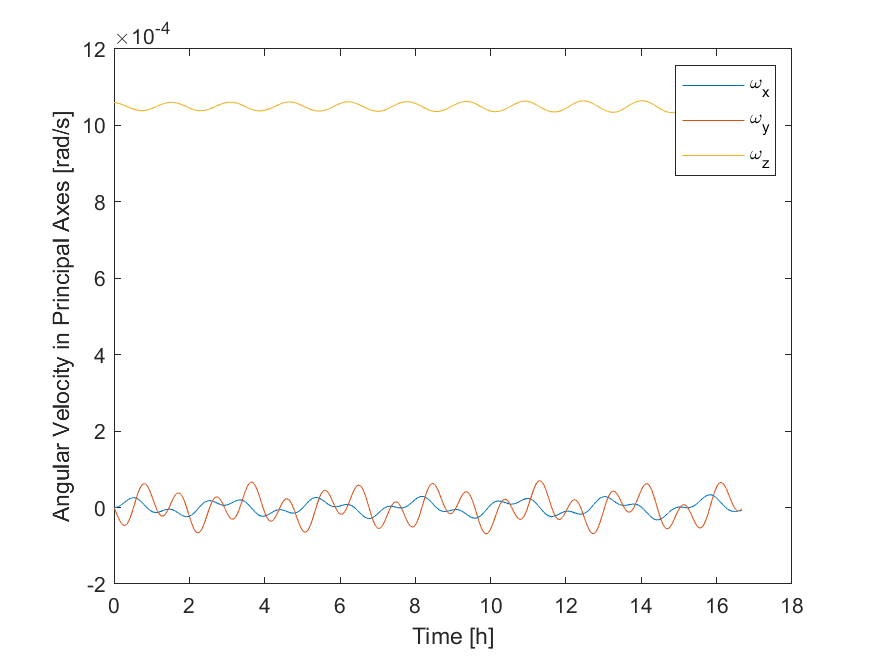
\includegraphics[scale=0.6]{Images/ps5_problem1c_angvel.png}
\caption{Angular velocity evolution for stable orientation with 1\% perturbations}
\label{fig:ps5_problem1c_angvel}
\end{figure}

As expected, our attitude motion (angular velocities and Euler angles) are periodically stable with a small perturbation in initial condition.

We cannot maintain this orientation if we want to properly point the radar antenna located at the top of the spacecraft, so it does not make sense to orient the satellite along principal axes for gravity gradient stability. Instead, we will likely require magnetorquers to offset angular momentum changes from environmental torques, including gravity gradient torques due to our unstable equilibrium.


\subsection{PROBLEM 2}
\textit{In addition to gravity gradient, start programming perturbation torques due to magnetic field, solar radiation pressure, and atmospheric drag. Note 1: You should apply a very minimal/basic model for perturbations that are not relevant (negligible) to your project. It is expected that you do not ignore them. Note 2: All perturbations can be grouped into a single large subsystem called environment or similar whose output feed
the Euler equations. Note 3: Re-use as many functions as possible for solar radiation pressure and atmospheric drag.}

In addition to gravity gradient torques, we modeled torque from magnetic field interactions, solar radiation pressure, and atmospheric drag.

The equation for the torque from the magnetic field interactions is shown below.

\begin{align*}
    \Vec{M}_{m} = \Vec{m}_{sat} \times \Vec{B}_{Earth}
\end{align*}

Since the satellite is operates in LEO, the spherical harmonic model up to n = 4 was used for maximum accuracy. This model is based on the geocentric distance ($R$), colatitude ($\theta$), and longitude ($\phi$). The model requires Gaussian coefficients ($g^{n,m}$, $h^{n,m}$) and Legendre functions ($P^{n,m}$) and their derivatives ($\frac{\delta P^{n,m} (\theta)}{\delta \theta}$), which are explained in more detail in Wertz \cite{Wertz}.

\begin{align*}
    B_R = \sum^{4}_{n=1} (\frac{R_{Earth}}{R})^{n+2} (n+1) \sum^{n}_{m=0}
    (g^{n,m} \cos{m \phi} + h^{n,m} \sin{m \phi}) P^{n,m}(\theta) \\
    B_{\theta} = - \sum^{4}_{n=1} (\frac{R_{Earth}}{R})^{n+2} \sum^{n}_{m=0}
    (g^{n,m} \cos{m \phi} + h^{n,m} \sin{m \phi}) \frac{\delta P^{n,m} (\theta)}{\delta \theta} \\
    B_{\phi} = - \frac{1}{\sin{\theta}} \sum^{4}_{n=1} (\frac{R_{Earth}}{R})^{n+2}
    \sum^{n}_{m=0} m (-g^{n,m} \sin{m \phi} + h^{n,m} \cos{m \phi}) P^{n,m}(\theta)
\end{align*}

The equations below define the solar radiation torque, where $C_S$ is the specular reflection coefficient, $C_d$ is the diffuse reflection coefficient, $\Vec{S}$ is the vector facing the Sun, and $e_i$ is 1 if the surface is illuminated and 0 otherwise. In implementation, we represent $e_i$ as a boolean tensor in tensor operations for fast computation.

\begin{align*}
    \Vec{M}_{S} = \sum^{n}_{i=1} \Vec{r}_{i} \times e_i \int_{S_i} d \Vec{f}_{total_{i}} \\
    d \Vec{f}_{total} = -P ((1-C_S) \hat{\Vec{S}} + 2 (C_S \cos{\theta} + \frac{1}{3} C_d) \cos{\theta} dA
\end{align*}

Finally, the equation below define the aerodynamic torque. Velocity is relative velocity of the spacecraft to the atmosphere, and we can compute the atmosphere's relative motion using a cross product of the position vector and Earth's rotational rate in ECI.

\begin{align*}
    d \Vec{f}_{aero} = - \frac{1}{2} C_D \rho V^2 (\hat{\Vec{V}} \cdot \hat{\Vec{N}}) \hat{\Vec{V}} dA
\end{align*}


The following function enables the propagation of the orbit with the specified perturbation torques.

\lstinputlisting{src/orbitTorque.m}
\lstinputlisting{src/drag.m}
\lstinputlisting{src/srp.m}
\lstinputlisting{src/magFieldTorque.m}

\subsection{PROBLEM 3}
\textit{Include all torques you have been able to model in numerical integration. Please show comparison of numerically computed disturbance torques with expected values and trend from theory (model) and tables (Wertz) referenced in class. Plot all torque components in principal axes over time. Plot the resultant (sum) of all torques in principal axes. Make sure that your model is not too ideal, i.e. make sure that center of pressure and center of mass do not coincide.}

For most torques, the worst-case estimated magnitudes were found by using existing properties of the spacecraft model. We use simplified equations (compared to those in the previous section) to estimate these, making assumptions for worst-case torques. However, the magnetic torque calculation assumes a model of the spacecraft's magnetic field as a single coil wrapped around the surface of the RIS and satellite bus. The estimated maximum values of each torque are listed in the table below.
t
\begin{table}[H]
\centering
\begin{tabular}{l|l} 

Magnetic Field & Estimated Maximum Value (N-m)  \\ 
\hline
$M_{gg}$          & 1.7093e-02                  \\ 
\hline
$M_{srp}$         & 1.8294e-02                  \\ 
\hline
$M_{drag}$        & 1.3682e-03                  \\ 
\hline
$M_{mag}$         & 1.3751e-10                  \\
\end{tabular}
\end{table}

In Figures \ref{fig:ps5_problem3_grav}, \ref{fig:ps5_problem3_drag}, \ref{fig:ps5_problem3_srp}, \ref{fig:ps5_problem3_mag}, we show the numerical simulation results for each type of disturbance based on the equations and code in the previous section. The numerical simulations indicate that the simulated results and estimated values are roughly within an order of magnitude for each type of disturbance torque shown.

\begin{figure}[H]
\centering
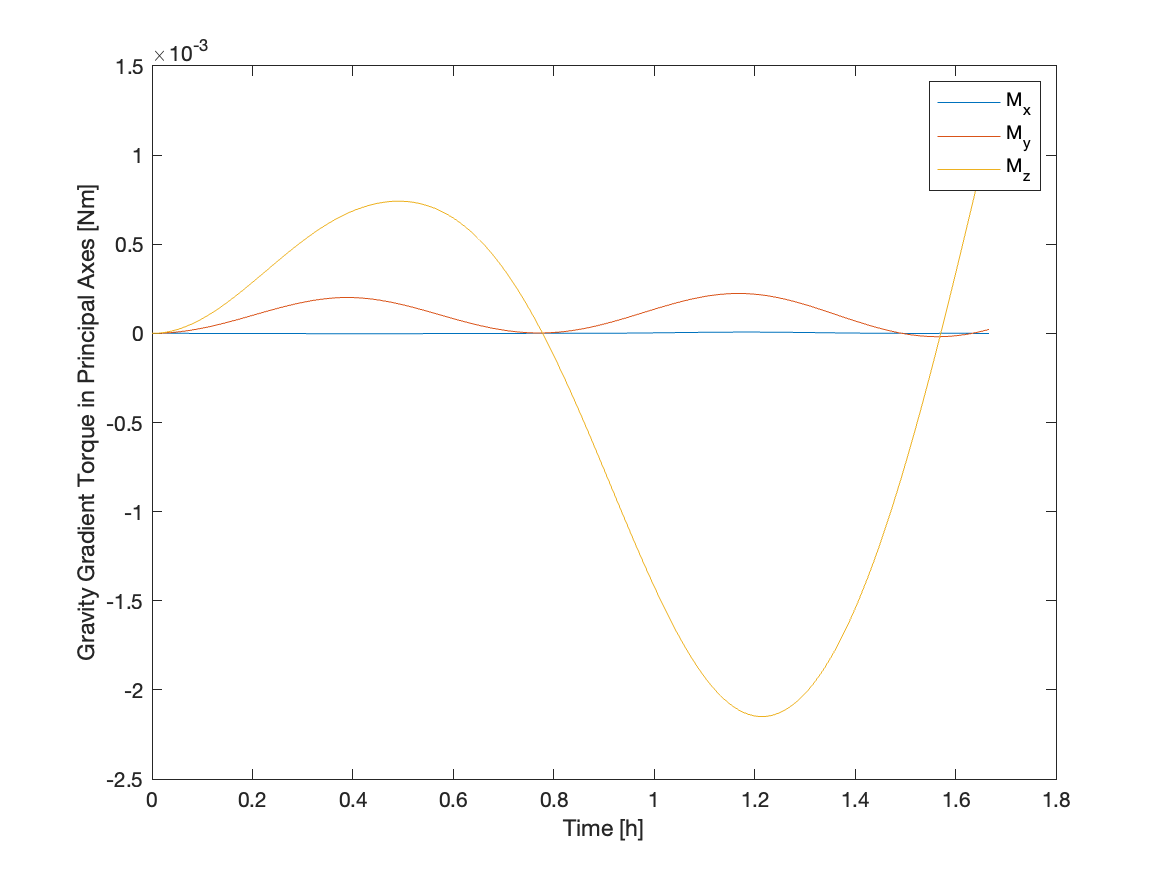
\includegraphics[scale=0.6]{Images/ps5_problem3_grav.png}
\caption{Numerical simulation of gravity gradient torques}
\label{fig:ps5_problem3_grav}
\end{figure}

\begin{figure}[H]
\centering
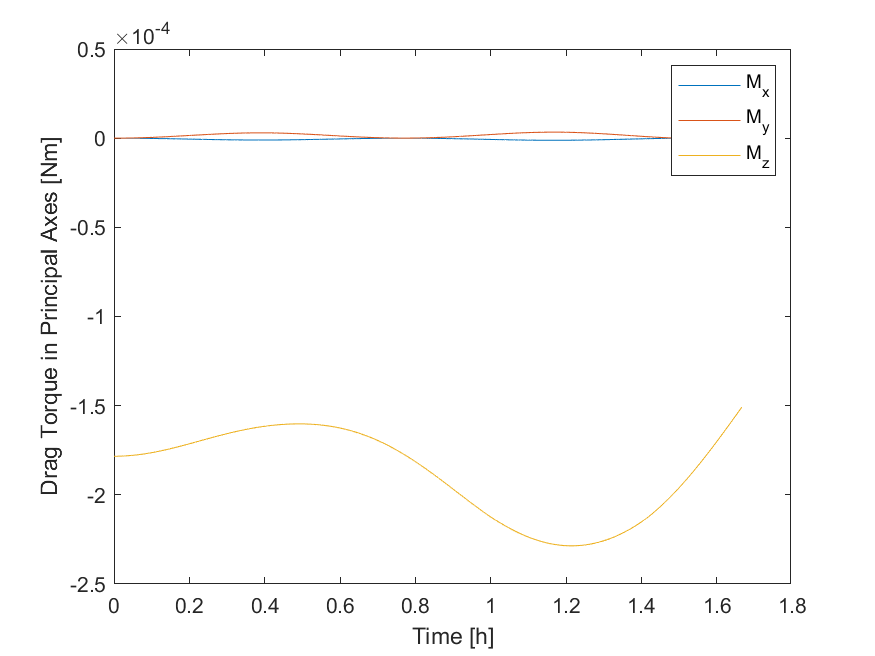
\includegraphics[scale=0.6]{Images/ps5_problem3_drag.png}
\caption{Numerical simulation of drag torques}
\label{fig:ps5_problem3_drag}
\end{figure}

\begin{figure}[H]
\centering
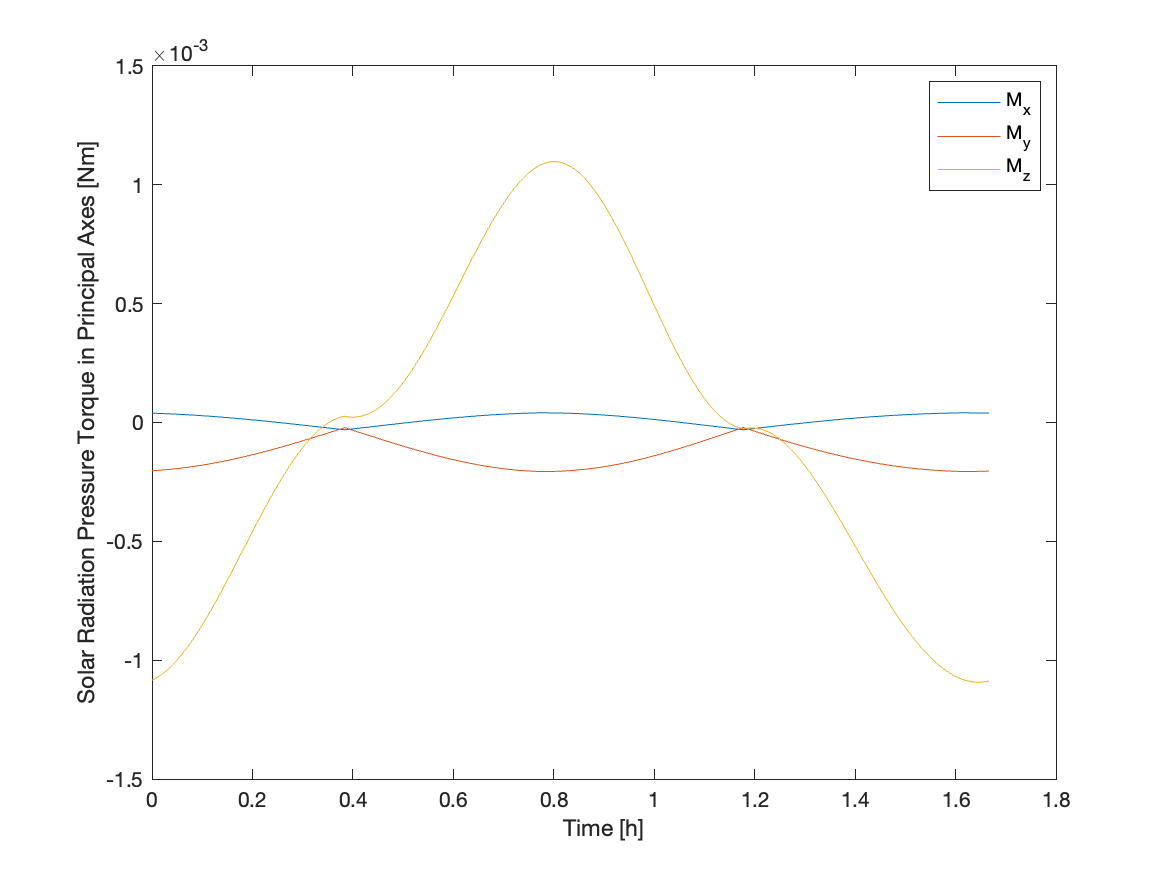
\includegraphics[scale=0.6]{Images/ps5_problem3_srp.png}
\caption{Numerical simulation of solar radiation pressure torques}
\label{fig:ps5_problem3_srp}
\end{figure}

\begin{figure}[H]
\centering
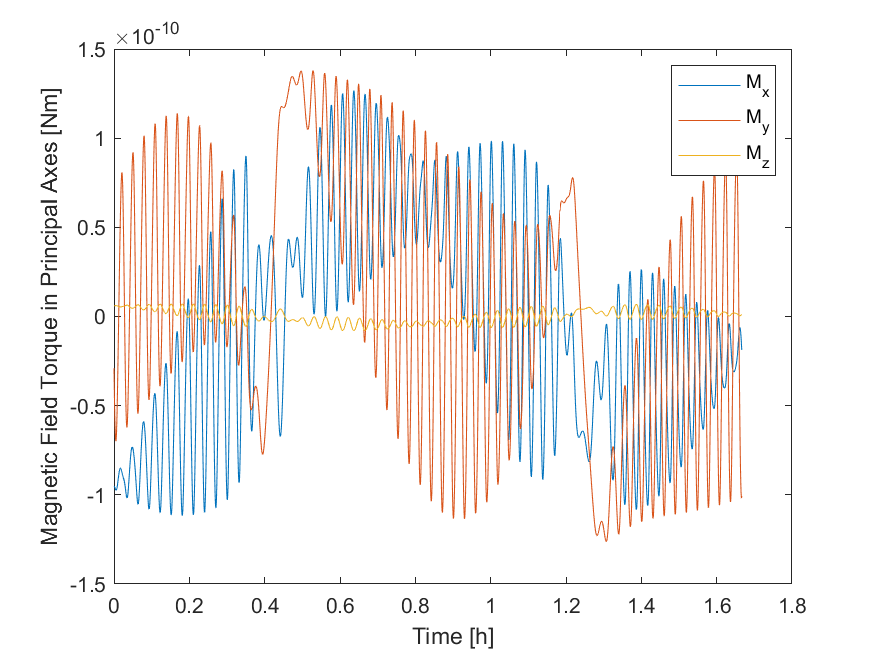
\includegraphics[scale=0.6]{Images/ps5_problem3_mag.png}
\caption{Numerical simulation of magnetic field torques}
\label{fig:ps5_problem3_mag}
\end{figure}

% \section{\Large PROBLEM SET 6}
\subsection{PROBLEM 1}
\textit{Complete the modeling and verification of perturbation torques as described in the previous pset}

We have implemented models of the drag, gravity gradient, magnetic field, and solar radiation pressure effects on our satellite. Please see the relevant portions of the previous section for more detail.


\subsection{PROBLEM 2}
\textit{Compute the attitude control error even if a controller is not implemented yet. The attitude control error represents the rotation between the desired and actual attitude. Plot the attitude control error and give its interpretation. Note that this step requires the definition and computation of the desired or nominal or target attitude of the spacecraft. In general, this can be expressed in body or principal axes.}

Given how the goal of the satellite is to have an Earth-pointing antenna, the ideal position for the satellite is to have the principal z-axis facing the negative radial direction. Additionally, to maximize solar coverage the principal y-axis should be aligned with the normal direction. Because of this, the desired attitude of the spacecraft should simply be the negative of the RTN frame, as shown below.

\begin{align*}
    \Vec{P}_{desired} &= 
    \begin{bmatrix}
    -1 & 0 & 0 \\
    0 & -1 & 0 \\
    0 & 0 & -1
    \end{bmatrix}
    \Vec{P}_{RTN}
\end{align*}

For the sake of this analysis, the simulated orbit was assumed to start off in the ideal attitude, and was assumed to have no torques. Figure \ref{fig:ps6_}

\subsection{PROBLEM 3}
\textit{Note that the attitude control error represents a rotation matrix (DCM) which quantifies how far the actual attitude is from the true attitude. You can use any parameterization to plot the attitude control errors corresponding to this DCM. Give interpretation of the attitude control errors given the applied disturbances.}

Show error with perturbation

\subsection{PROBLEM 4}
\textit{You can now start modeling the Simulink spacecraft subsystem which is what the satellite believes is happening (on-board). Initially, the sensors provide ideal measurements (no bias or noise). Just use an empty box for those. The outputs of the sensors are measurements which are used for attitude determination. These measurements are computed from the reference truth or oracle.}

\subsection{PROBLEM 5}
\textit{Assume a certain set of sensors. In general, a number of unit vectors and angular velocities can be considered as measurements}

\textit{Implement the deterministic attitude determination algorithm discussed in class and its variant which uses fictitious measurements to spread the errors across the measurements}

\textit{Implement the statistical attitude determination algorithm discussed in class (q-method)}

\textit{Implement angular velocity measurements and the reconstruction of the attitude from those (through kinematic equations coded identically to ground truth but replicated in the spacecraft on-board computer)}

\subsection{PROBLEM 6}
\textit{Plot the resulting estimated attitude in the absence of sensor errors. Show that it is identical to the true attitude (except for numerical errors).}

% \section{\Large PROBLEM SET 7}
\subsection{PROBLEM 1}
\textit{Introduce representative (from manufacturer or Wertz or first lectures) sensor errors in the form of constant bias and Gaussian noise with given standard deviation.}

Given how the actual sensors used in NISAR are not public information, much of the sensor error and bias information was extrapolated from data from Wertz and lecture materials and manufacturers making similar sensors for similar satellites. The table below includes the general sensor information used in this analysis.

\begin{table}[H]
\begin{tabular}{|l|l|l|}
\hline
\textbf{Sensor} & \textbf{Sensor Error} & \textbf{Sensor Bias} \\ \hline
Sun Sensor \cite{Wertz} & 0.5 \degree & 0 \degree \\ \hline
Star Tracker \cite{Wertz} & 0.01 \degree & 0 \degree \\ \hline
Gyroscope \cite{CVGGyro} & 0.001 \degree / s & 5e-5 \degree / s \\ \hline
\end{tabular}
\end{table}

\subsection{PROBLEM 2}
\textit{Re-apply the attitude determination algorithms from the previous pset. Plot attitude estimation error. Note that the attitude estimation error represents a rotation matrix (DCM) which quantifies how far the estimated attitude is from the true attitude. You can use any parameterization to plot the attitude estimation errors corresponding to this DCM. Is the result consistent with the sensor bias and noise you have introduced?}

The estimation errors for the Deterministic Attitude Method, q Method, and kinematics-based method are plotted below. As expected, the q Method has significantly lower error than the Deterministic Attitude Method. Additionally, since the gyroscopes were modeled to have a slight bias, we see that the euler angles slowly drift away from expected values.

\begin{figure}[H]
\centering
\includegraphics[scale=0.6]{Images/.png}
\caption{Attitude evolution based on MEKF time update}
\label{fig:ps7_problem5a_angle_est}
\end{figure}

\begin{figure}[H]
\centering
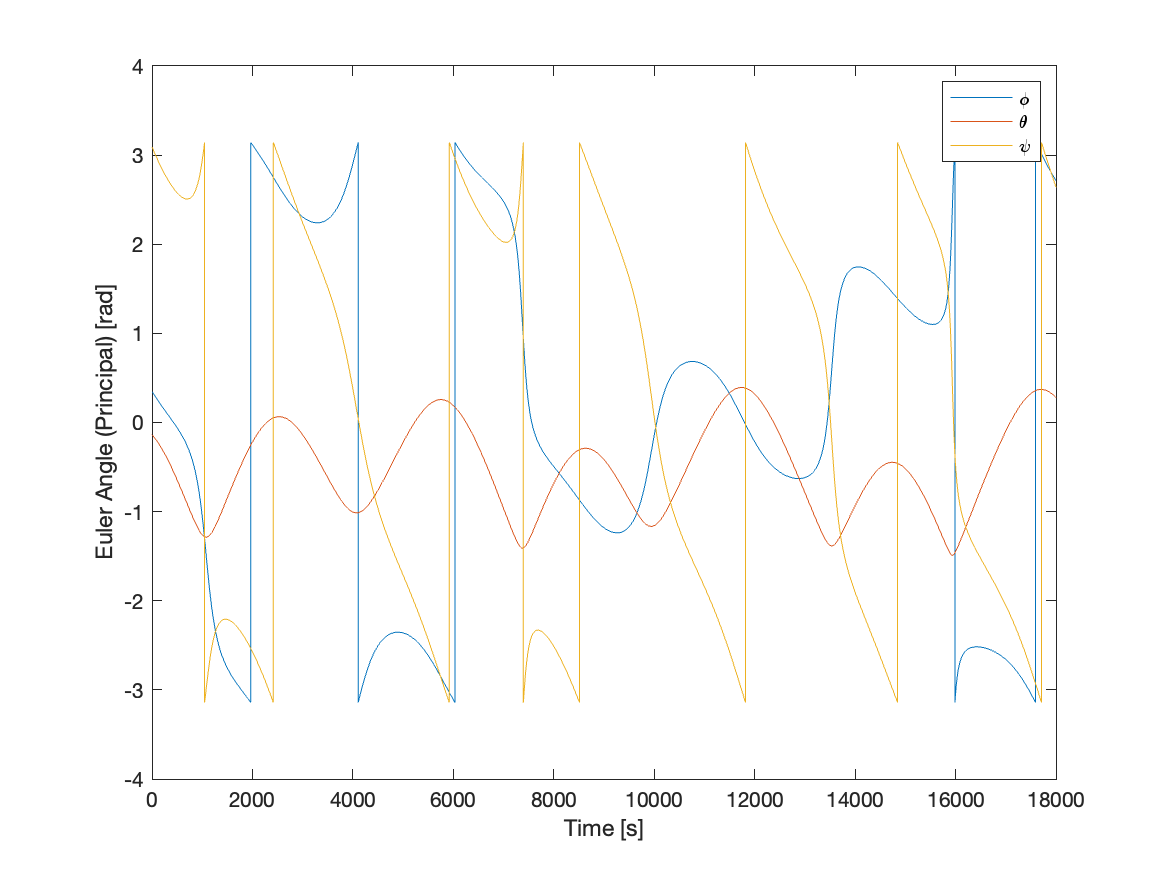
\includegraphics[scale=0.6]{Images/ps7_problem5a_angle_est.png}
\caption{Attitude evolution based on MEKF time update}
\label{fig:ps7_problem5a_angle_est}
\end{figure}

\begin{figure}[H]
\centering
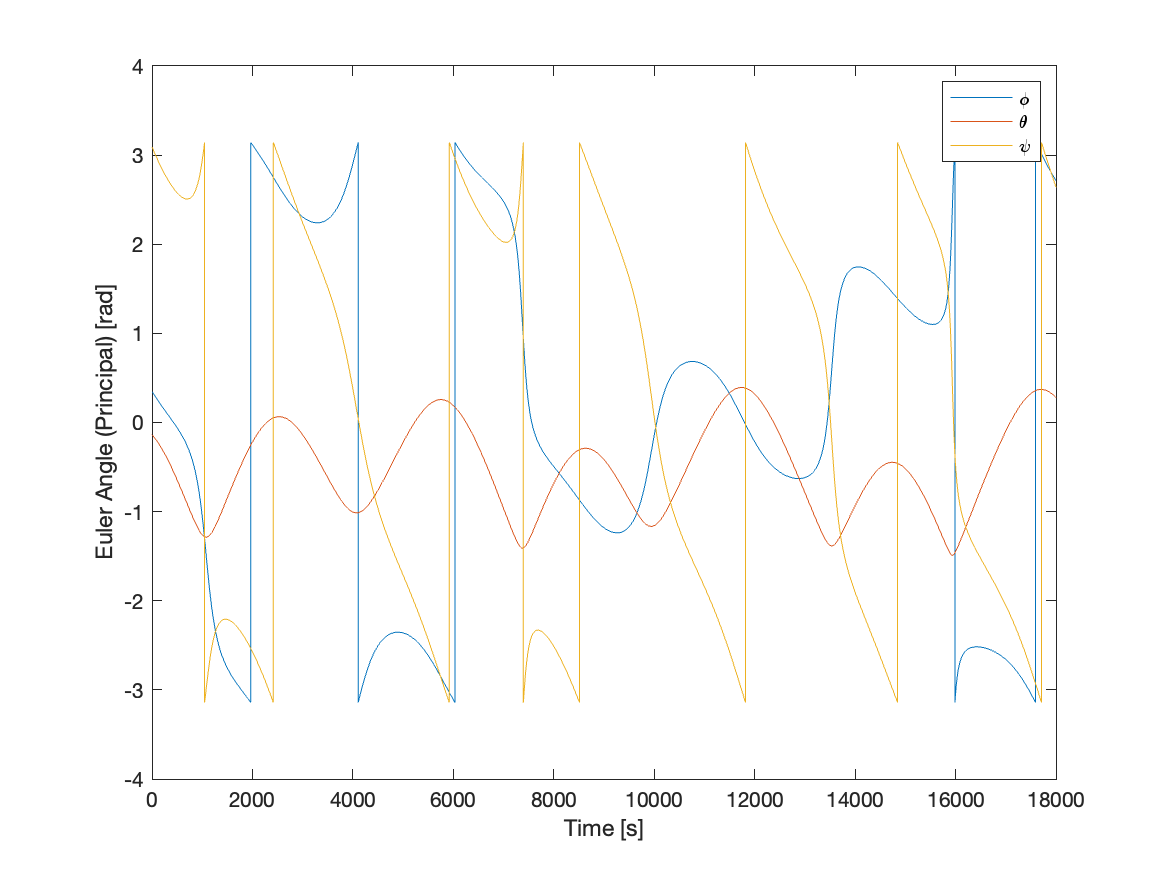
\includegraphics[scale=0.6]{Images/ps7_problem5a_angle_est.png}
\caption{Attitude evolution based on MEKF time update}
\label{fig:ps7_problem5a_angle_est}
\end{figure}

\subsection{PROBLEM 3}
\textit{For small sensor errors, the DCM corresponds to a small rotation. Can you give an interpretation of small angles (e.g., in Euler angles and quaternions) to the obtained error DCM?}

\subsection{PROBLEM 4}
\textit{Start modeling actual sensors in dedicated (Simulink or otherwise) subsystems which are part of the spacecraft. These models take inputs from ground-truth simulation and provides output measurements, including systematic and random errors. Take inspiration from overview of sensors discussed in class and textbook for typical errors.}

\subsection{PROBLEM 5}
\textit{Designing and implement the time update of a KF/EKF to obtain the best estimate of the state from the available measurements and models:}

The following MATLAB function is our time update-only implementation of a multiplicative extended Kalman filter (MEKF). We describe the formulation of the MEKF immediately following this function.

\lstinputlisting{src/timeUpdate.m}

\textit{Search in literature, define, and code a state transition matrix $\Phi$ which provides your state at step k+1 based on the state at step k. Verify that the output of this propagation step is consistent with the rigorous propagation of the attitude (numerical integration). Plot propagation errors as needed.}

Our state consists of 3 small angles (zero mean) and angular velocities. Our state does not track the attitude directly, but we can compute quaternions using known kinematics.
\begin{align*}
    \Vec{x} = \begin{bmatrix}
        \alpha_{x} & \alpha_{y} & \alpha_{z} & \omega_{x} & \omega_{y} & \omega{z}
    \end{bmatrix}^{\intercal}
\end{align*}

The small angle component of our state is reset every iteration and not updated in the time update step \cite{CubeSatTelescope}.
\begin{align*}
    A &= I_{3} + \frac{s_{\omega}}{\omega} [\Vec{\omega}_{t} \times] + \frac{1 - c_{\omega}}{\omega^{2}} [\Vec{\omega}_{t} \times] [\Vec{\omega}_{t} \times] \\
    \Phi_{\omega} & = I_{3} + \Delta t \begin{bmatrix}
        0 & \frac{I_{y} - I_{z}}{I_x} \omega_{z_{t}} & \frac{I_{y} - I_{z}}{I_x} \omega_{y_{t}} \\
        \frac{I_{z} - I_{x}}{I_y} \omega_{z_{t}} & 0 & \frac{I_{z} - I_{x}}{I_y} \omega_{x_{t}} \\
        \frac{I_{x} - I_{y}}{I_z} \omega_{y_{t}} & \frac{I_{x} - I_{y}}{I_z} \omega_{x_{t}} & 0
    \end{bmatrix} \\
    \Phi &= \begin{bmatrix}
        A & 0 \\
        0 & \Phi_{\omega}
    \end{bmatrix}
\end{align*}

Since we are using a MEKF, we propagate the quaternion attitude representation outside of the state vector. The quaternion attitude is propagated by $\Omega (\Vec{\omega})$, identical to the quaternion kinematics used previously.

We plot the attitude from our MEKF and our numerical integration simulation, respectively. Upon inspection, these plots appear identical. Small errors in the simulation are analyzed later in Problem 6.

\begin{figure}[H]
\centering
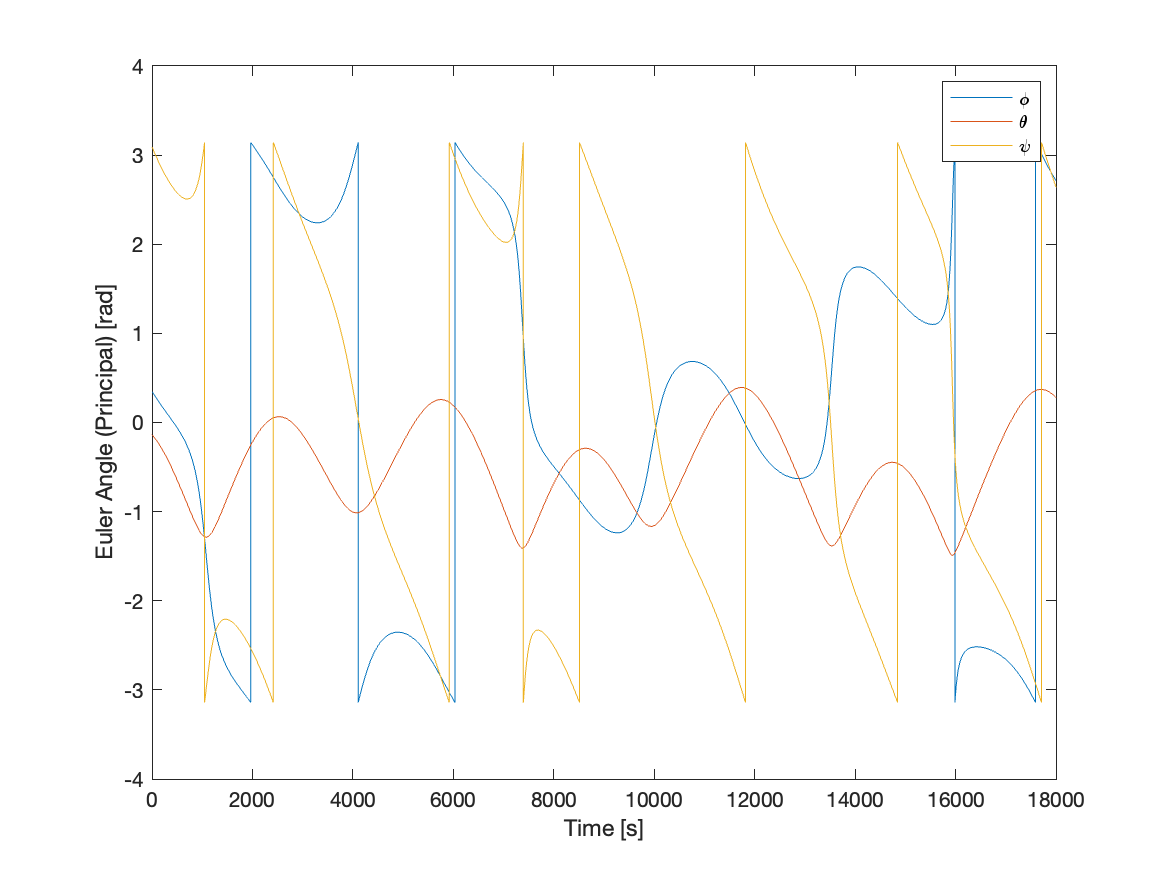
\includegraphics[scale=0.6]{Images/ps7_problem5a_angle_est.png}
\caption{Attitude evolution based on MEKF time update}
\label{fig:ps7_problem5a_angle_est}
\end{figure}

\begin{figure}[H]
\centering
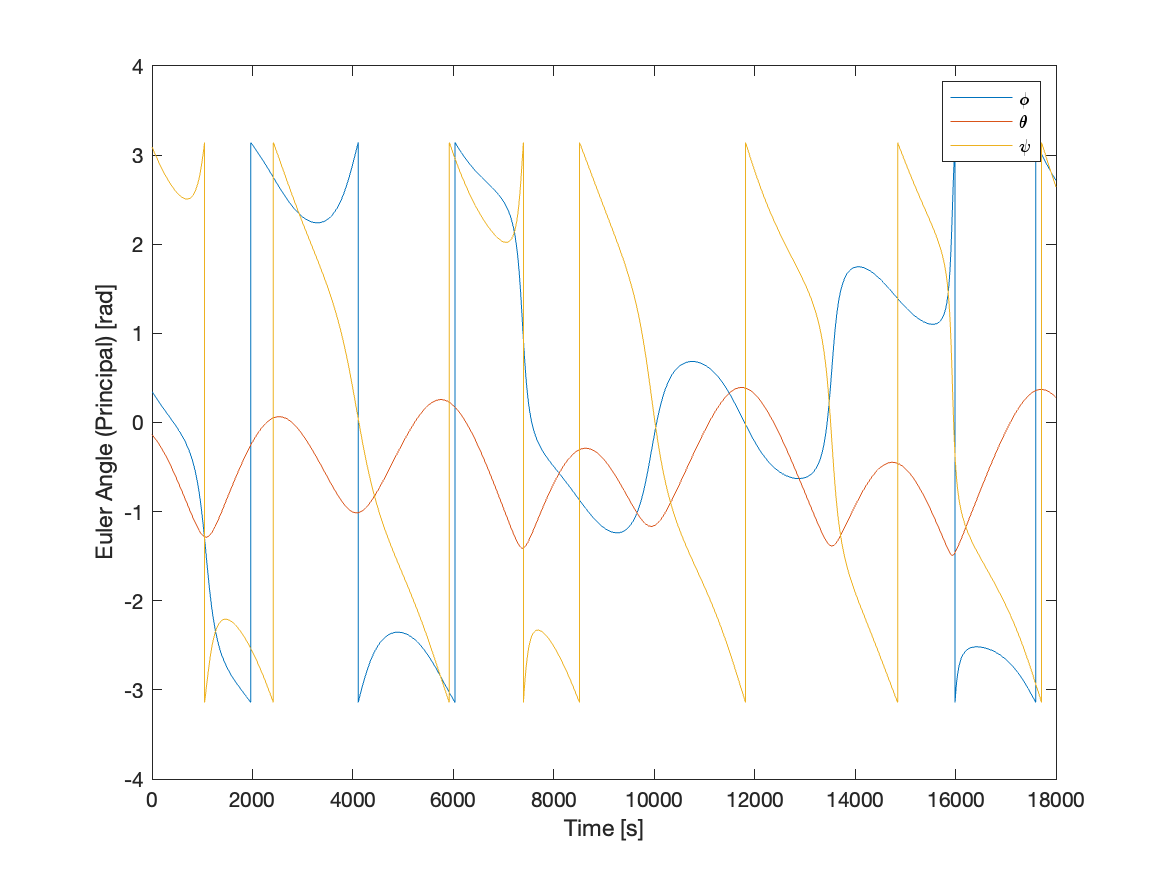
\includegraphics[scale=0.6]{Images/ps7_problem5a_angle_sim.png}
\caption{Attitude evolution from "ground truth" simulation}
\label{fig:ps7_problem5a_angle_sim}
\end{figure}

We also plot the angular velocity from both the MEKF time update step and the numerical simulation. As with the attitude evolution, both plots appear to be the same. Note that we do not include perturbations in our simulation in our comparison, as the state would quickly diverge otherwise because the measurement update is not yet implemented in the MEKF.

\begin{figure}[H]
\centering
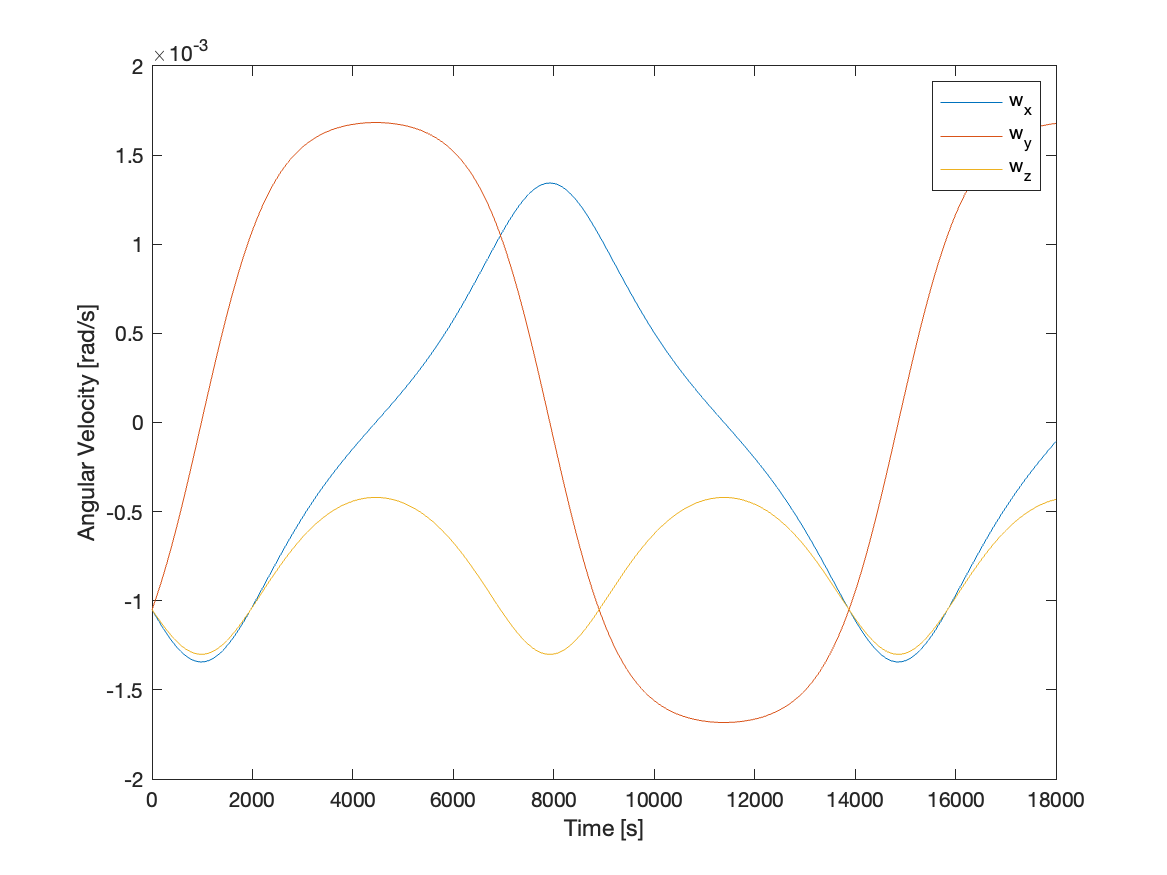
\includegraphics[scale=0.6]{Images/ps7_problem5a_angvel_est.png}
\caption{Angular velocity based on MEKF time update}
\label{fig:ps7_problem5a_angvel_est}
\end{figure}

\begin{figure}[H]
\centering
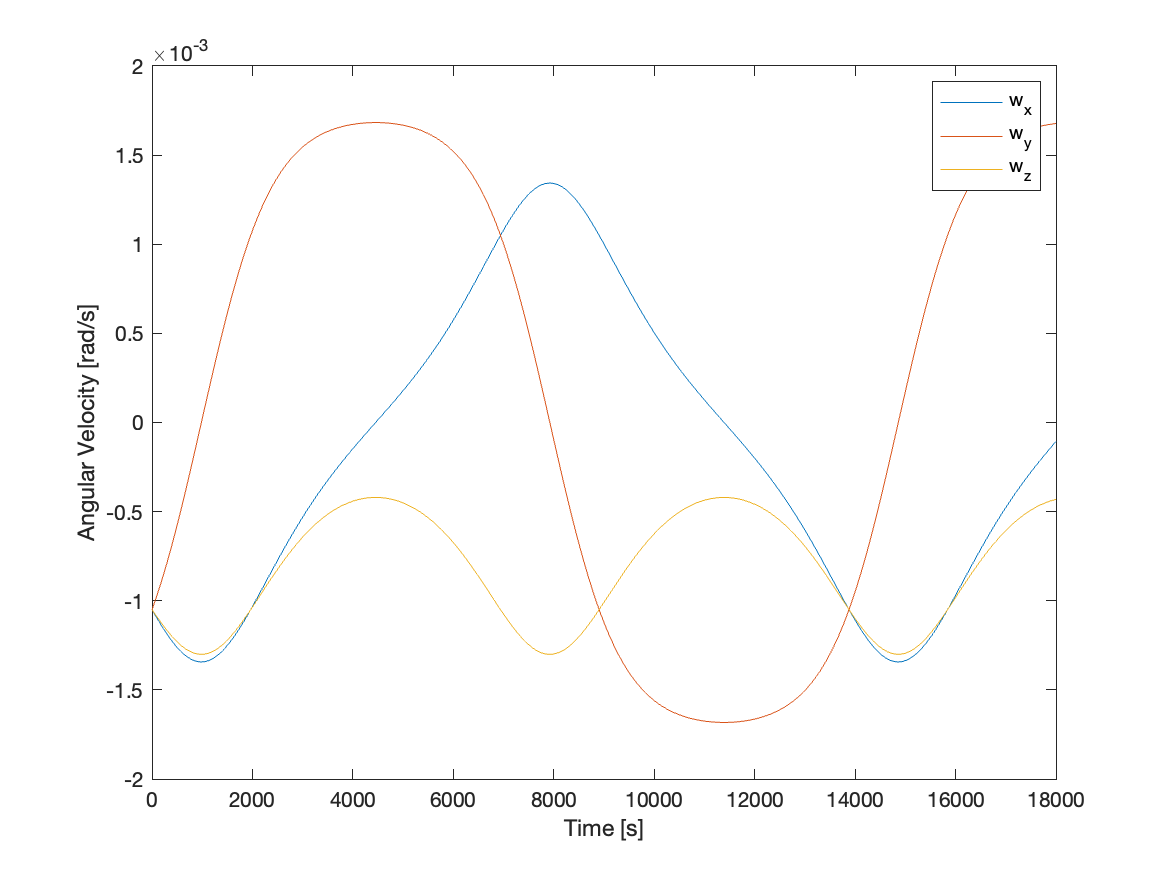
\includegraphics[scale=0.6]{Images/ps7_problem5a_angvel_sim.png}
\caption{Angular velocity from "ground truth" simulation}
\label{fig:ps7_problem5a_angvel_sim}
\end{figure}

\textit{Search in literature, define, and code a control input matrix B which provides the increment to your state at step k+1 due to a control torque at step k. Hint: optional at this stage since you do not have a controller yet.}

For now, we choose to model our control inputs as torque inputs (moments) about the principal axes. Thus, we can choose a $B$ matrix as follows:

\begin{align*}
    u &= \begin{bmatrix}
        M_{x} & M_{y} & M_{z}
    \end{bmatrix}
    B &= \begin{bmatrix}
        \frac{1}{I_{x}} & 0 & 0 \\
        0 & \frac{1}{I_{y}} & 0 \\
        0 & 0 & \frac{1}{I_{z}}
    \end{bmatrix}
\end{align*}

\textit{(a) and (b) allow you to propagate the state from k to k+1 including the known control input torques. Hint: Initially you will design the filter by neglecting any control torque from your simulation.}

\textit{Define and code an initial state error covariance matrix P which quantifies the uncertainty of your initial state. This can be picked as diagonal matrix with diagonal elements representing the variance of each state parameter $\sigma^{2}$. Initially you can neglect cross-covariance terms assuming that errors of various state components are not correlated.}

\textit{The time update of the EKF needs $\Phi$, B, and P. Hint: You could increment your navigation performance by keeping the filter receptive to new measurements at steady state through the addition of constant process noise Q at each step. Initially you can define Q similar to P but much smaller (e.g., 1/10 or 1/100).}

\subsection{PROBLEM 6}
\textit{Produce plots showing true attitude estimation errors (estimate vs truth with statistics), formal or estimated attitude estimation errors (covariance from filter). Discuss the results, do they meet expectations? How well is the true estimation error described by the formal covariance? Note that we are only implementing the time update even if we call them “attitude estimates and estimation errors”.}

\begin{figure}[H]
\centering
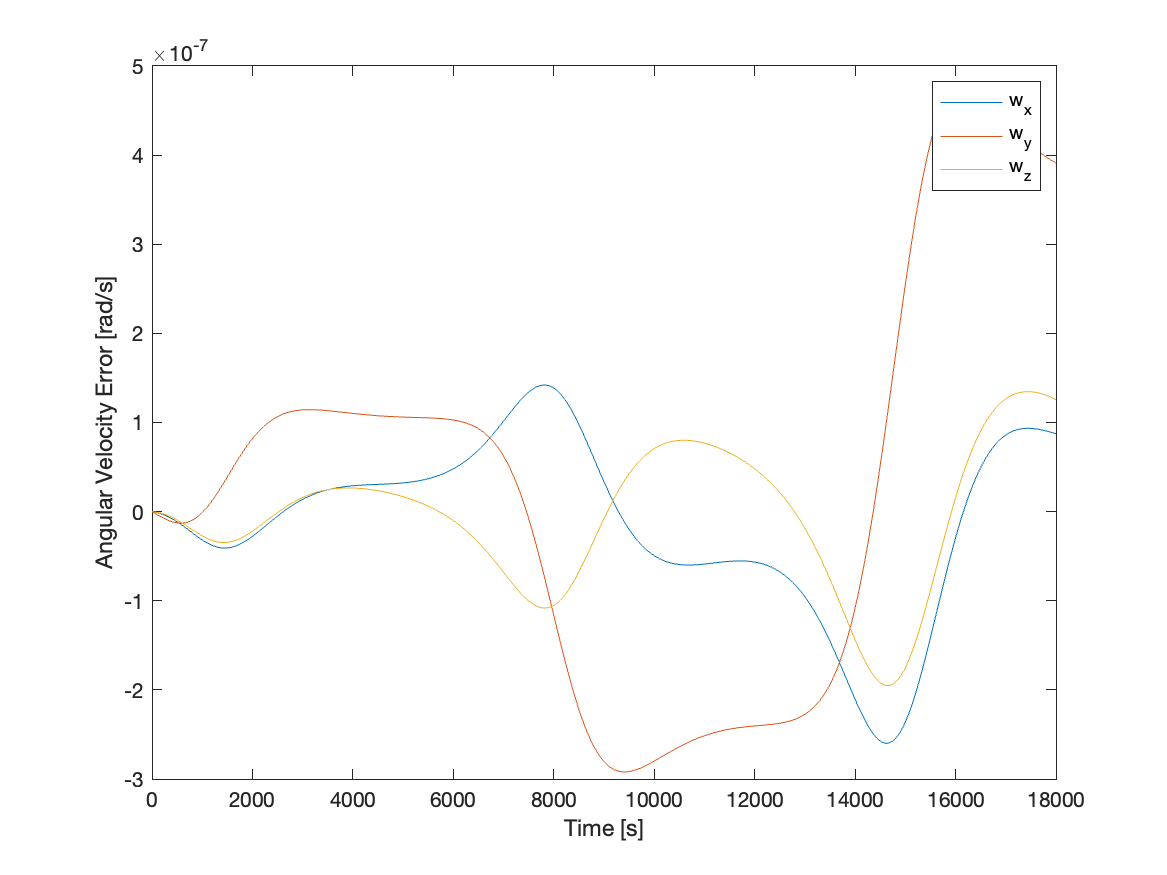
\includegraphics[scale=0.6]{Images/ps7_problem6_angvel_err.png}
\caption{Attitude error between estimate and simulation}
\label{fig:ps7_problem5a_angvel_sim}
\end{figure}

\begin{figure}[H]
\centering
\includegraphics[scale=0.6]{Images/ps7_problem6_angle_err.png}
\caption{Angular velocity error between estimate and simulation}
\label{fig:ps7_problem5a_angvel_sim}
\end{figure}

% \section{\Large PROBLEM SET 8}
\subsection{PROBLEM 1}
\textit{The time update should be complete and verified at this stage. We need to include the incoming measurements. Search in literature or derive, define, and code a sensitivity matrix \textbf{H} which provides your state at step k+1 from your measurement vector at step k+1 (i.e., at the same current time, propagation has already been done).}

The following equations define the sensitivity matrix $\mathbf{H_k}$, for the case where there are $n$ vector measurements (sun sensors, star trackers, etc.), and 1 gyroscope vector reading.

\begin{align*}
    \mathbf{H} = \frac{\delta \mathbf{h}}{\delta \mathbf{x}} =
    \begin{bmatrix}
        [\mathbf{h_1} \times] & \mathbf{0}_{3 \times 3} \\
        [\mathbf{h_2} \times] & \mathbf{0}_{3 \times 3} \\
        ... & ... \\
        [\mathbf{h_n} \times] & \mathbf{0}_{3 \times 3} \\
        \mathbf{0}_{3 \times 3} & \mathbf{I}_{3 \times 3} \\
    \end{bmatrix}
\end{align*}

In the equation above, $[\mathbf{h_i} \times]$ refers to the cross-product matrix for the measurement vector $\mathbf{h_i}$.

\subsection{PROBLEM 2}
\textit{Define and code your constant measurement error covariance matrix \textbf{R} which quantifies the uncertainty of your measurements. This can be picked as diagonal matrix with diagonal elements representing the variance of each parameter $\sigma^{2}_{m}$. Hint: If your instrument is well characterized you can use $\sigma_{m}$ applied in your simulation to generate the measurements from your ground-truth.}

For the sensors used in our measurements, $\mathbf{R}$ was defined as a diagonal matrix of the sensor variances discussed in Problem Set 7 Problem 1 (where the sensor errors are the standard deviations of the white noise in each case).

\begin{align*}
    \mathbf{R} = 
    \begin{bmatrix}
        diag(\sigma_{star tracker}^2) & \mathbf{0} & \mathbf{0} \\
        \mathbf{0} & diag(\sigma_{sun sensor}^2) & \mathbf{0} \\
        \mathbf{0} & \mathbf{0} & diag(\sigma_{gyroscopes}^2)\\
    \end{bmatrix}
\end{align*}

\subsection{PROBLEM 3}
\textit{Compute your modelled measurement vector at step k+1 from your state at step k+1. This transformation can be rigorous (non-linear, EKF) or approximate (linear, KF).}

The modeled measurement vector at step k+1 was found by plugging the estimated state at step k+1 into the previously developed measurement model, without measurement noise.

\subsection{PROBLEM 4}
\textit{Compute your pre-fit residuals \textit{z} by differencing modelled and actual measurement vector at k+1.}

The pre-fit residuals were calculated based on the output of the measurements acquired with noise and the measurements from the measurement models.

\subsection{PROBLEM 5}
\textit{The measurement update of the EKF needs \textbf{H}, \textbf{P}, \textbf{R}, and \textbf{z} to compute the Kalman gain \textbf{K}, the new estimated state and its associated covariance matrix.}

The following equations are used in the measurement step calculation.

\begin{align*}
    \mathbf{x_{k+1 | k+1}} = \mathbf{x_{k+1 | k}} + \mathbf{K_k}
    (\mathbf{y_k} - \mathbf{z_k}) \\
    \mathbf{P_{k+1 | k+1}} = \mathbf{P_{k+1 | k}} - 
    \mathbf{K_k} \mathbf{H_k} \mathbf{P_{k+1 | k}} \\
    \mathbf{K_k} = \mathbf{P_{k+1 | k}} \mathbf{H_k}^T [\mathbf{H_k} \mathbf{P_{k+1 | k}} \mathbf{H_k}^T + \mathbf{R_k}]^{-1}
\end{align*}


\subsection{PROBLEM 6}
\textit{Compute your post-fit residuals z by differencing modelled and actual measurement vector at k+1 using your new state. These should be smaller than the pre-fit residuals and should capture the standard deviation of your measurements at steady state.}

The post-fit residuals z are found by taking the updated state from the measurement update and plugging them into the noiseless measurement model again. Figures \ref{} below show the difference in the norms of the pre-fit and post-fit residuals. As expected, the post-fit residuals are slightly smaller than the pre-fit residuals; however, this can definitely be improved.


\subsection{PROBLEM 7}
\textit{Produce plots showing true attitude estimation errors (estimate vs truth with statistics at steady state), formal or estimated attitude estimation errors (covariance from filter), pre- and post-fit residuals (with statistics at steady state), etc. Discuss the results, do they meet expectations? Is the true estimation error well described by the formal covariance? Are the measurements residuals consistent with the applied measurement errors? Hint: show estimation errors, do not overlap state estimate with reference truth.}

\subsection{PROBLEM 8}
\textit{Start thinking/planning possible upgrades for the final project deliverable. Upgrades can go in several directions tailored to your project needs. For example, define different modes for attitude estimation using different sensors and algorithms based on your concept of operations. What would it take to implement a UKF instead of an EKF? Can you improve your dynamics and measurement models? Can you use measurements that are more representative of what your sensors are going to actually provide you? Hint: you should not panic if your Kalman filter is not working, you can always address the rest of the problem sets bypassing the Kalman filter. Do not give up though!}

One possible upgrade for the final project could be to compute pointing for Earth remote sensing–that is, determining where to point the satellite 

% \section{\Large PROBLEM SET 9}
\subsection{PROBLEM 1}
\textit{Start selecting and sizing your actuators using the basic dimensional formulas provided in class (Wertz,SMAD) based on your perturbation environment and attitude slew objectives. Provide rationale for choice.}

\subsection{PROBLEM 2}
\textit{Start modeling actuators in dedicated (Simulink) subsystems which are part of the spacecraft. These models take inputs from ground-truth simulation and provides output control torques to be directly fed into the Euler equations, including systematic and random errors. Plot output vs input of actuator model. Hint: for the rest of this problem set you should remove all sensing and actuation errors for verification purposes.}

\subsection{PROBLEM 3}
\textit{Start designing and implementing a linear control law which provides the desired behavior of the dynamic system (damping and frequency) by a feedback done on the control tracking errors. Try using both a small angle approximation and a non-linear approach in defining the control tracking errors used in the control law. Hint: this task requires that you linearize the Euler equations and that you show how the gains of the linear control law are derived, also start applying the control law by assuming that the actuators are doing their job ideally (no actuation equations, no saturation or other limits). Selection of gains can be done through standard PD, pole placement or LQR approaches.}

\subsection{PROBLEM 4}
\textit{Start plotting all the relevant quantities of your simulation, including attitude determination errors, attitude control errors, control actions (along all axes), etc. Hint: stress difference between what the ADCS believes, and what the spacecraft is actually doing. This affects estimation, control errors, and control actions.}

\section{\Large INTRODUCTION}
Our mission will utilize a satellite with synthetic aperture radar (SAR), designed to gather key remote sensing and environmental data for the Earth. The satellite will be in low Earth orbit (LEO) and use quaternions to describe its orientation, avoiding gimbal lock effects of other conventions. For state estimation, the spacecraft will require gyroscopes, star trackers, and a potentially a sun sensor. For actuation, the spacecraft will likely utilize thrusters, reaction wheels, and magnetorquers.

\subsection{Literature Review}
Space agencies such as NASA have been constructing SAR satellites to gather satellite images and data of Earth for over a decade. Additionally, there exist commercial entities also utilizing SAR in their spacecraft.

For example, Soil Moisture Active Passive (SMAP) is a NASA satellite launched in 2015 that utilizes L-band synthetic aperture radar (SAR) technology to measure soil moisture from LEO. This data has applications in climate change research climate change research applications (such as updating climate models) and some day-to-day activities (such as improving weather forecasts). SMAP is unique in that it had a large deployable reflector, held above the spacecraft body by a deployable boom \cite{SMAP}.

Companies EOS and Capella Space are also developing satellites that use SAR technology in the X-band and S-band frequencies for commercial applications ranging from agriculture to mining \cite{EOSSAR, Capella}. The commercial applicability of SAR is substantial, especially as SAR can penetrate cloud cover while generating high-resolution data, making it superior to many other forms of remote sensing technology. EOS claims to obtain resolution of up to 0.25 m, while Capella Space claims a capability of up to 0.5 m. These satellites all operate in LEO, which enables high-frequency monitoring of the Earth's surface.

NASA and ISRO have partnered to create a SAR satellite as well. The joint project between NASA JPL and ISRO has resulted in the NASA-ISRO Synthetic Aperture Radar (NISAR), a satellite that captures data in the L-band and S-band SAR frequencies \cite{NISARMission}. NISAR's high resolution will permit the detailed measurement of the Earth's surface, enabling better observation of changes in Earth's crust for disaster prevention and mitigation. NISAR will also support science goals such as monitoring ice sheets and the oceans, and its orbit is designed to cover the entire Earth every 12 days.

\subsection{Mission Selection}
NISAR is a joint Earth-observation satellite mission between NASA and ISRO. It is the first satellite to operate in two different Synthetic Aperture Radar (SAR) bands, incorportating both L- and S-band SAR instruments. Both frequencies can penetrate clouds for reliable data collection, but the L-band can also penetrate thicker vegetation that the S-band cannot. Uniquely, NISAR is intended to be used for a wide range of science objectives, including disaster response and agriculture \cite{NISARApps}.

\section{\Large SPECIFICATIONS}
\subsection{Requirements}
NISAR is a joint Earth-observation satellite mission between NASA and ISRO. It is the first satellite to operate in two different Synthetic Aperture Radar (SAR) bands, incorportating both L- and S-band SAR instruments. Both frequencies can penetrate clouds for reliable data collection, but the L-band can also penetrate thicker vegetation that the S-band cannot. Uniquely, NISAR is intended to be used for a wide range of science objectives, including disaster response and agriculture \cite{NISARApps}.

NISAR ADCS requirements are \textless 273 arcseconds for pointing and \textless 500 m for orbit control \cite{Siqueira}. The satellite duty cycle is specified as \textgreater 30\%. NISAR will operate in LEO with nominal altitude of 747 km and 6 AM/6 PM orbit. NISAR's L- and S-band instruments operate at 24 cm and 12 cm wavelengths, respectively. NISAR collects terrestial SAR imagery with an image swatch of 240 km using a sweep approach. The science payload can also perform polarimetry, with the SAR incorporating multiple polarization modes.

\subsection{Layout}
\begin{figure}[H]
\centering
\includegraphics[scale=0.38]{Images/nisar_diagram.jpg}
\caption{The basic components of the NISAR satellite}
\label{NISAR Diagram}
\end{figure}

As shown in Figure \ref{NISAR Diagram}, NISAR's satellite consists of a 1.2 m x 1.8 m x 1.9 m spacecraft bus cuboid with a 1.2 m wide octagonal Radar Instrument Structure (RIS). The spacecraft bus includes ADCS hardware, power subsystem, and engineering payload, while the RIS houses hardware for the L- and S-band SAR. The satellite is powered by 23 m\textsuperscript{2} of solar panels, consisting of an array of two panels, one on each side of the satellite. Additionally, a 12 m diameter radar antenna is positioned above the body of the spacecraft, attached by a 9 m long boom. This boom consists of beams with 7 in x 7 in cross-section area \cite{NISARMission}.

Table \ref{tab:mass} contains mass properties of the satellite. Unfortunately, detailed mass distribution and inertia properties of NISAR are not openly available, so we provide estimates of mass distribution based on known overall component-level masses. We are given total masses for the bus structure and RIS, and we also know the masses of the payloads located within, allowing us to compute an accurate mass for these components \cite{NISARMission}. We estimate that solar panels have a mass of 23 kg each based on knowledge that NISAR's solar panels are 23 m\textsuperscript{2} and a typical solar panel mass per area is 2.06 kg/m\textsuperscript{2} \cite{SolarPanelMass}. We know that the entire radar antenna assembly has a mass of 292 kg, and we estimate that the reflector has a mass of approximately 100 kg based on a similar deployable SAR S- and L-band mesh antenna reflector \cite{L3Harris}. We will use these masses to compute center of mass and moments of inertia in the following section. For our model, we neglect the effects of the truss structure supporting the antenna reflector, instead modeling the entire RAR as just the disk-shaped reflector mesh.

\begin{longtable}{l|r}
\caption{Mass of NISAR components}
\label{tab:mass}\\
\textbf{Components}              & \multicolumn{1}{l}{\textbf{Mass [kg]}} \\ \hline
\endfirsthead
%
\endhead
%
Bus                              & 964.1                                      \\
Radar Instrument Structure (RIS) & 1375.9                                     \\
Solar Panel +y                   & 23                                         \\
Solar Panel -y                   & 23                                         \\
Radar Antenna Boom (RAB)         & 192                                        \\
Radar Antenna Reflector (RAR)    & 100                                       
\end{longtable}

Since NISAR is a remote sensing satellite requiring high attitude control performance, it has an ADCS system with an array of sensors and actuators. Sensors include star sensors, sun sensors, GPS, and a 3-axis gyroscope for roll, pitch, and yaw. For actuators, NISAR has four 50 N$\cdot$m reaction wheels mounted in tetrahedral configuration, three 565 and 350 A$\cdot$m\textsuperscript{2} magnetorquers, and fourteen thrusters (ten canted 11 N thrusters, one central 11 N thruster, and four 1 N thrusters for roll) \cite{NISARMission}.

\subsection{Mass Properties}
We simplify the spacecraft geometry into six components, each individually assumed to have uniform mass distribution. These components of the simplified geometry are: bus structure (including ADCS hardware and engineering payload), RIS (Radar Instrument Structure), RAB (radar antenna boom), RAR (radar antenna reflector), and two solar panels (identified as the +y solar panel and -y solar panel). The bus structure is modeled as a rectangular prism, while the RIS is modeled as an octagonal prism. The RAB is also modeled as a rectangular prism, while the RAR is modeled as a thin disk and the solar panels are modeled as thin rectangular plates. Within each geometry, our model assumes mass is distributed uniformly. From analyzing diagrams found in technical reports, we estimate that the RAR is tilted -3.87\degree{} about the y-axis (relative to the x-axis), while the RAB is modeled as a single beam with an angle approximately -18\degree{} from vertical (from the z-axis, about the y-axis in the x-z plane). Note that we have simplified the shape of the RAB from a beam of two angled segments to a single, straight beam.

We choose the body axes to have an origin at the center of the rectangular bus. This configuration is chosen because the bus houses the ADCS hardware, including actuators and sensors. The x-axis points in the direction of the RIS, and the z-axis points up vertically, normal to the upper surface of the bus. See Figure \ref{fig:MATLAB_model} for a visual depiction of the body axes relative to the spacecraft.

We compute the center of mass after extracting the centroid of each component. The mass of each component is previously found in Table \ref{tab:mass}. The centroid of each component is listed in Table \ref{tab:centroid}.

\begin{longtable}{l|r|r|r}
\caption{Component centroids [m]}
\label{tab:centroid}\\
\textbf{Part} & \multicolumn{1}{l}{\textbf{x}} & \multicolumn{1}{l}{\textbf{y}} & \multicolumn{1}{l}{\textbf{z}} \\ \hline
\endfirsthead
%
\endhead
%
Bus      & 0     & 0    & 0    \\
RIS      & 1.85  & 0    & 0    \\
Panel +y & 0     & 3.9  & 0    \\
Panel -y & 0     & -3.9 & 0    \\
RAB      & -0.899 & 0    & 5.194 \\
RAR      & 4.283   & 0    & 8.308
\end{longtable}

The center of mass can be found by taking the weighted average of each component centroid, weighted by the mass of each component. The center of mass formula is:

\begin{equation*}
    \Vec{r}_{cm} = \frac{\sum m_{i} \Vec{r}_{i}}{\sum m_{i}}
\end{equation*}

This yields a result for center of mass at $\qty[parse-numbers = false]{[1.046, 0, 0.683]}{\metre}$ relative to the origin we defined. We use a MATLAB script to compute the center of mass from a CSV file containing centroid and mass data.

We compute the moment of inertia of the satellite, finding an inertia tensor in our body axes. To do this, we break the satellite into individual components, first finding the moment of inertia about the center of mass of each component. We then compute the moment of inertia of the entire satellite about the body axes by using parallel axis theorem and combining all the components.

To compute the moment of inertia, we need the following geometric properties of each component:

\begin{longtable}{l|r|r|r|r|r}
\caption{Dimensions of modeled components [m]}
\label{tab:dimensions}\\
\textbf{Part} & \textbf{L (x-dim)} & \textbf{W (y-dim)} & \textbf{H (z-dim)} & \textbf{S (oct. side length)} & \textbf{R (radius)} \\ \hline
\endfirsthead
%
\endhead
%
Bus &  & 1.8 & 1.9 & - & - \\
RIS & 2.5 & - & - & 0.459 & - \\
Panel +y & - & 6 & 1.9 & - & - \\
Panel -y & - & 6 & 1.9 & - & - \\
RAB & 0.1778 & 0.1778 & 9 & - & - \\
RAR & - & - & - & - & 6
\end{longtable}

For the bus, we choose to model the geometry as a rectangular prism. Since the bus is aligned with the body axes, we obtain a diagonal inertia tensor:

\begin{align*}
I_{bus} &=
\begin{bmatrix}
I_{xx} & 0 & 0 \\
0 & I_{yy} & 0 \\
0 & 0 & I_{zz}
\end{bmatrix} \\
&=
\begin{bmatrix}
m \frac{W^{2} + H^{2}}{12} & 0 & 0 \\
0 & m \frac{L^{2} + H^{2}}{12} & 0 \\
0 & 0 & m \frac{L^{2} + W^{2}}{12} 
\end{bmatrix} \\
&=
\qty[parse-numbers = false]{
\begin{bmatrix}
550.340 & 0 & 0 \\
0 & 405.725 & 0 \\
0 & 0 & 375.9993 
\end{bmatrix}
}{\kilogram\metre\squared}
\end{align*}

For the solar panels, we approximate their geometry as a flat plate. These axes are also aligned, so the tensor can be diagonal.

\begin{align*}
I_{panel} &=
\begin{bmatrix}
I_{xx} & 0 & 0 \\
0 & I_{yy} & 0 \\
0 & 0 & I_{zz}
\end{bmatrix} \\
&=
\begin{bmatrix}
m \frac{W^{2} + H^{2}}{12} & 0 & 0 \\
0 & m \frac{H^{2}}{12} & 0 \\
0 & 0 & m \frac{W^{2}}{12} 
\end{bmatrix} \\
&=
\qty[parse-numbers = false]{
\begin{bmatrix}
75.919 & 0 & 0 \\
0 & 6.919 & 0 \\
0 & 0 & 69 
\end{bmatrix}
}{\kilogram\metre\squared}
\end{align*}

For the RIS, we model the geometry as an octagonal prism. For the moment of inertia about the axisymmetric axis of the octagon, we use the formula $m \left(\frac{S^{2}}{24} + \frac{a^{2}}{2}\right)$, where $S$ is the side length and $a$ is the apothem length, where the apothem is the perpendicular length from a side of the octagon to the center \cite{McCarron}. When calculating the moment of inertia about the non-axisymmetric axes, we approximate the geometry as a cylinder with radius equal to the average of the octagonal radius (distance from center to vertex) and the apothem. As will be shown later, this approximation yields a very close result to the inertia tensor generated from the CAD model.

\begin{align*}
I_{RIS} &=
\begin{bmatrix}
I_{xx} & 0 & 0 \\
0 & I_{yy} & 0 \\
0 & 0 & I_{zz}
\end{bmatrix} \\
&=
\begin{bmatrix}
m \left(\frac{S^{2}}{24} + \frac{a^{2}}{2}\right) & 0 & 0 \\
0 & m \left(\frac{L^{2}}{12} + \frac{R_{avg}^{2}}{4}\right) & 0 \\
0 & 0 & m \left(\frac{L^{2}}{12} + \frac{R_{avg}^{2}}{4}\right) 
\end{bmatrix} \\
&=
\qty[parse-numbers = false]{
\begin{bmatrix}
223.268 & 0 & 0 \\
0 & 831.089 & 0 \\
0 & 0 & 831.089 
\end{bmatrix}
}{\kilogram\metre\squared}
\end{align*}

For the RAB, we first model the geometry as a rectangular prism. We also must rotate the inertia tensor to match the orientation of the body axes, as the RAB itself is rotated relative to the bus about the y-axis by -18\degree{} from vertical (z-axis).

\begin{align*}
I_{RAB} &=
\begin{bmatrix}
I_{xx} & 0 & 0 \\
0 & I_{yy} & 0 \\
0 & 0 & I_{zz}
\end{bmatrix} \\
&=
\begin{bmatrix}
m \frac{W^{2} + H^{2}}{12} & 0 & 0 \\
0 & m \frac{L^{2} + H^{2}}{12} & 0 \\
0 & 0 & m \frac{L^{2} + W^{2}}{12} 
\end{bmatrix} \\
&=
\qty[parse-numbers = false]{
\begin{bmatrix}
1296.506 & 0 & 0 \\
0 & 1296.506 & 0 \\
0 & 0 & 1.012 
\end{bmatrix}
}{\kilogram\metre\squared}
\end{align*}

We apply the rotation to the inertia tensor using a rotation matrix about the y-axis. Note that doing so results in non-zero products of inertia, meaning our principal axes will not be aligned with our body axes.

\begin{align*}
I_{RAB,rotated} &= R_{y}(-18\degree) I_{RAB} R_{y}^{\intercal}(-18\degree) \\
&=
\qty[parse-numbers = false]{
\begin{bmatrix}
1172.797 & 0 & 380.736 \\
0 & 1296.506 & 0 \\
380.736 & 0 & 124.720
\end{bmatrix}
}{\kilogram\metre\squared}
\end{align*}

Finally, we model the RAR as a flat disk. Similar to the RAB, we must rotate the inertia tensor to match the orientation of the body axes.

\begin{align*}
I_{RAR} &=
\begin{bmatrix}
I_{xx} & 0 & 0 \\
0 & I_{yy} & 0 \\
0 & 0 & I_{zz}
\end{bmatrix} \\
&=
\begin{bmatrix}
m \frac{R^{2}}{4} & 0 & 0 \\
0 & m \frac{R^{2}}{4} & 0 \\
0 & 0 & m \frac{R^{2}}{2} 
\end{bmatrix} \\
&=
\qty[parse-numbers = false]{
\begin{bmatrix}
900 & 0 & 0 \\
0 & 900 & 0 \\
0 & 0 & 1800 
\end{bmatrix}
}{\kilogram\metre\squared}
\end{align*}

Applying a rotation:

\begin{align*}
I_{RAR,rotated} &= R_{y}(-3.87\degree) I_{RAR} R_{y}^{\intercal}(-3.87\degree) \\
&=
\qty[parse-numbers = false]{
\begin{bmatrix}
904.100 & 0 & -60.605 \\
0 & 900 & 0 \\
-60.605 & 0 & 1795.900
\end{bmatrix}
}{\kilogram\metre\squared}
\end{align*}

Now, we use parallel axis theorem to compute the moment of inertia of each component about the body axes at the specified origin. We can use the following displacement tensor,

\begin{equation*}
D =
\begin{bmatrix}
y^{2} + z^{2} & -xy & -xz \\
-yx & x^{2} + z^{2} & -yz \\
-zx & -yz & x^{2} + y^{2}
\end{bmatrix},
\end{equation*}

where $x$, $y$, $z$ are the coordinates of the center of mass of the component, giving the moment of inertia about a new point:

\begin{equation*}
    I' = I_{c} + mD
\end{equation*}

Performing the parallel axis theorem on each component and summing the inertia tensors, we obtain the following inertia tensor for the entire spacecraft:

\begin{equation*}
I_{NISAR,body} =
\qty[parse-numbers = false]{
\begin{bmatrix}
15783.996 & 0 & -2341.659 \\
0 & 22227.752 & 0 \\
-2341.659 & 0 & 10663.970
\end{bmatrix}
}{\kilogram\metre\squared}
\end{equation*}

Compare this with the inertia tensor computed by SolidWorks CAD software:

\begin{equation*}
I_{NISAR,body} =
\qty[parse-numbers = false]{
\begin{bmatrix}
15780.361 & 0 & -2336.285 \\
0 & 22225.721 & 0 \\
-2336.285 & 0 & 10665.796
\end{bmatrix}
}{\kilogram\metre\squared}
\end{equation*}

The errors are 0.0230\%, 0.00914\%, 0.0171\%, and 0.230\% for $I_{xx}$, $I_{yy}$, $I_{zz}$, and $I_{xz}$, respectively. We created the following MATLAB script to compute the inertia tensor.

\subsection{Surface Properties}
For the purpose of discretizing the spacecraft into surfaces, we consider the outer faces of the bus, RIS, and RAB. We also consider the faces of the solar panels and RAR, which are modeled as thin plates. The centroid (barycenter) coordinates and area for each surface are obtained using the surface properties tool in SolidWorks, and a unit normal vector is manually computed based on the orientation of the surface. We then enter this data into a CSV file, which can be read into MATLAB.

This function stores the data into arrays of barycenter coordinates, unit normal vector components, and area. Each row of an array corresponds to a particular surface. The data is shown in Table \ref{tab:surfaces}, annotated with the identity of each surface.

\begin{longtable}{l|r|r|r|r|r|r|r}
\caption{Surface parameters}
\label{tab:surfaces}\\
 &
  \multicolumn{3}{c}{\textbf{Barycenter [m]}} &
  \multicolumn{3}{c}{\textbf{Normal}} &
  \multicolumn{1}{l}{} \\
\endfirsthead
%
\endhead
%
\textbf{Surface} &
  \multicolumn{1}{l}{\textbf{x}} &
  \multicolumn{1}{l}{\textbf{y}} &
  \multicolumn{1}{l}{\textbf{z}} &
  \multicolumn{1}{l}{\textbf{x}} &
  \multicolumn{1}{l}{\textbf{y}} &
  \multicolumn{1}{l}{\textbf{z}} &
  \multicolumn{1}{l}{\textbf{Area [m\textsuperscript{2}]}} \\ \hline
Bus front, minus RIS (+x) & 0.6   & 0     & 0     & 1      & 0      & 0      & 2.4   \\
Bus rear (-x)                  & -0.6  & 0     & 0     & -1     & 0      & 0      & 3.42  \\
Bus side (+y)                  & 0     & 0.9   & 0     & 0      & 1      & 0      & 2.28  \\
Bus side (-y)                  & 0     & -0.9  & 0     & 0      & -1     & 0      & 2.28  \\
Bus top (+z)                   & 0     & 0     & 0.95  & 0      & 0      & 1      & 2.16  \\
Bus bottom (-z)                & 0     & 0     & -0.95 & 0      & 0      & -1     & 2.16  \\
RIS front (+x)                 & 3.1   & 0     & 0     & 1      & 0      & 0      & 1.02  \\
RIS top (+z)                   & 1.85  & 0     & 0.55  & 0      & 0      & 1      & 1.15  \\
RIS bottom (-z)                & 1.85  & 0     & -0.55 & 0      & 0      & -1     & 1.15  \\
RIS side (+y)                  & 1.85  & 0.55  & 0     & 0      & 1      & 0      & 1.15  \\
RIS side (-y)                  & 1.85  & -0.55 & 0     & 0      & -1     & 0      & 1.15  \\
RIS angle face (y-z I)         & 1.85  & 0.39  & 0.39  & 0      & 0.707  & 0.707  & 1.15  \\
RIS angle face (y-z II)        & 1.85  & -0.39 & 0.39  & 0      & -0.707 & 0.707  & 1.15  \\
RIS angle face (y-z III)       & 1.85  & -0.39 & -0.39 & 0      & -0.707 & -0.707 & 1.15  \\
RIS angle face (y-z IV)        & 1.85  & 0.39  & -0.39 & 0      & 0.707  & -0.707 & 1.15  \\
Panel +y front (+x)            & 0     & 3.9   & 0     & 1      & 0      & 0      & 11.4  \\
Panel +y rear (-x)             & 0     & 3.9   & 0     & -1     & 0      & 0      & 11.4  \\
Panel -y front (+x)            & 0     & -3.9  & 0     & 1      & 0      & 0      & 11.4  \\
Panel -y rear (-x)             & 0     & -3.9  & 0     & -1     & 0      & 0      & 11.4  \\
RAB front (x-z, +x)            & -0.81 & 0     & 5.21  & 0.951  & 0      & 0.309  & 1.6   \\
RAB rear (x-z, -x)             & -0.99 & 0     & 5.18  & -0.951 & 0      & -0.309 & 1.6   \\
RAB side (+y)                  & -0.9  & -0.09 & 5.19  & 0      & 1      & 0      & 1.6   \\
RAB side (-y)                  & -0.9  & 0.09  & 5.19  & 0      & -1     & 0      & 1.6   \\
RAB top (+z)                   & -2.31 & 0     & 9.47  & 0      & 0      & 1      & 0.03  \\
RAR top (+z)                   & 4.28  & 0     & 8.31  & -0.067 & 0      & 0.998  & 113.1 \\
RAR bottom (-z)                & 4.28  & 0     & 8.31  & 0.067  & 0      & -0.998 & 113.1
\end{longtable}

\subsection{Body Axes}
A 3D model of the spacecraft is shown in Figure \ref{fig:complex_model}. The model shown is a screen capture from the SolidWorks CAD software.

\begin{figure}[H]
\centering
\includegraphics[scale=0.4]{Images/ps1_complex_model.png}
\caption{A 3D model of the satellite}
\label{fig:complex_model}
\end{figure}


We also show a simplified model of the spacecraft in Figure \ref{fig:simple_model}. This is the model we use to compute our mass and surface properties.

\begin{figure}[H]
\centering
\includegraphics[scale=0.4]{Images/ps1_simple_model.png}
\caption{A 3D model of the simplified satellite geometry}
\label{fig:simple_model}
\end{figure}

We also plot the model in MATLAB by importing an STL version of the CAD model. We show the body axes in Figure \ref{fig:MATLAB_model}, with the origin chosen as the center of the spacecraft bus.

\begin{figure}[H]
\centering
\includegraphics[scale=0.7]{Images/ps1_model.png}
\caption{Satellite model in MATLAB with body axes shown}
\label{fig:MATLAB_model}
\end{figure}

\subsection{Principal Axes}
The unit vectors of the principal axes with respect to the body axes ($\Vec{e}_i$) and the inertia tensor in the principal axes ($I_i$) can be found by taking the eigenvalue decomposition of the inertia tensor in the body axis. This can be seen in the two equations below.

\begin{equation*}
    I_i \cdot \Vec{e}_i = I_i \cdot \Vec{I}_{body} \\ \hspace{1cm} i = x, y, z
\end{equation*}

\begin{align*}
\Vec{I}_{principal} &= 
    \begin{bmatrix}
    I_x & 0 & 0 \\
    0 & I_y & 0 \\
    0 & 0 & I_z 
    \end{bmatrix}
= 
\qty[parse-numbers = false]{
    \begin{bmatrix}
    7707.07 & 0 & 0 \\
    0 & 14563.2 & 0 \\
    0 & 0 & 18050.4 
    \end{bmatrix}
}{\kilogram\metre\squared}
\end{align*}

We follow convention $I_z > I_y > I_x$ for defining principal axes.

The unit vectors of the principal axes ($\Vec{e}_i$) can then be used to find the rotation matrix ($\Vec{R}$), as shown below.

\begin{align*}
\Vec{R} &= 
    \begin{bmatrix}
    \Vec{e}_x & \Vec{e}_y & \Vec{e}_z 
    \end{bmatrix}
= 
    \begin{bmatrix}
    -0.06278 & -0.99803 & 0 \\
    0 & 0 & 1 \\
    -0.99803 & 0.06278 & 0 
    \end{bmatrix} \\
    \Vec{I}_{body} &= \Vec{R} \Vec{I}_{principal} \Vec{R}^{\intercal}
\end{align*}

\begin{figure}[H]
\centering
\includegraphics[scale=0.7]{Images/ps2_model.png}
\caption{Principal axes at center of mass (green) and body axes at origin (red)}
\label{fig:ps2_model}
\end{figure}

\section{\Large DYNAMICS}
\subsection{Orbit}

From the science users' handbook, we obtain the following orbital elements \cite{NISARHandbook}.

\begin{table}[H]
\begin{tabular}{lllllll}
\textbf{OE} & \textit{a} & \textit{e} & \textit{i} & \textit{$\Omega$} & \textit{$\omega$} & \textit{$\nu$} \\ \hline
\textbf{Value} & 7125.48662 km & 0.0011650 & 98.40508$\degree$ & -19.61601$\degree$ & 89.99764$\degree$ & -89.99818$\degree$
\end{tabular}
\end{table}

We convert these using a MATLAB function into ECI coordinates that can be fed into a numerical orbital propagator. Notice that we first convert the orbital elements a, e, and $\nu$ into perifocal (PQW) coordinates, using a and e to find the semi-latus rectum and a, e, and $\nu$ to find the distance to the central body (Earth). Then, we perform a series of rotations on these coordinates parameterized by $\omega$, i, and $\Omega$ to obtain new coordinates in the ECI frame.

Then, we can numerically propagate in MATLAB using \texttt{ode113} using a function that computes the time derivative of the ECI state. This is accomplished simply by setting the time derivative of position equal to the velocity portion of the state and setting the time derivative of velocity equal to an acceleration computed using the law of universal gravitation. Note that while our propagator does not include disturbance forces, it will be easy to incorporate these later. See the appendix corresponding to Problem Set 2 for application of \texttt{ode113}.

Now, we plot the trajectory for one orbit in Figure \ref{fig:simple_propagator}. Plotting multiple orbits (for example, over 12 days) yields the same plot, as \texttt{ode113} is very stable for this application.

\begin{figure}[H]
\centering
\includegraphics[scale=0.7]{Images/ps2_problem1.png}
\caption{A single orbit for NISAR in ECI coordinates (no perturbations)}
\label{fig:simple_propagator}
\end{figure}

\subsection{Euler Equations}
Initially, we represent our dynamics using simplified Euler equations. We use the following equations with zero external moments ($M_{x}, M_{y}, M_{z} = 0$).

\begin{align*}
    I_{x} \Dot{\omega}_{x} + (I_{z} - I_{y}) \omega_{y} \omega_{z} &= M_{x} \\
    I_{y} \Dot{\omega}_{y} + (I_{x} - I_{z}) \omega_{z} \omega_{x} &= M_{y} \\
    I_{z} \Dot{\omega}_{z} + (I_{y} - I_{x}) \omega_{x} \omega_{y} &= M_{z}
\end{align*}

We choose arbitrary initial conditions $\omega_{x} = \qty{8}{\degree\per\second}$, $\omega_{y} = \qty{4}{\degree\per\second}$, and $\omega_{z} = \qty{6}{\degree\per\second}$. The results of numerical integration using \texttt{ode113} are shown in Figure \ref{fig:ps2_euler_equations}.

\begin{figure}[H]
\centering
\includegraphics[scale=0.6]{Images/ps2_euler_equations.png}
\caption{Results from numerical integration of Euler equations}
\label{fig:ps2_euler_equations}
\end{figure}

\subsection{Energy Ellipsoid}
We use the energy ellipsoid to visualize our dynamics. We compute our surface using rotational kinetic energy based on initial conditions and principal axes inertia tensor.

\begin{align*}
    &2T = \omega_{x}^{2} I_{x} + \omega_{y}^{2} I_{y} + \omega_{z}^{2} I_{z} \\
    &\frac{\omega_{x}^{2}}{2T/I_{x}} + \frac{\omega_{y}^{2}}{2T/I_{y}} + \frac{\omega_{z}^{2}}{2T/I_{z}} = 1
\end{align*}

For the given initial conditions, we get semi-major axes of the following lengths: $\omega_{x} = \qty{0.2332}{\radian\per\second}$, $\omega_{y} = \qty{0.1697}{\radian\per\second}$, and $\omega_{z} = \qty{0.1524}{\radian\per\second}$. These values make sense given the equation for the energy ellipsoid.

Similarly, we compute our surface for the momentum ellipsoid with angular momentum based on our initial conditions and the principal axes inertia tensor.

\begin{align*}
    &L = \omega_{x}^{2} I_{x}^{2} + \omega_{y}^{2} I_{y}^{2} + \omega_{z}^{2} I_{z}^{2} \\
    &\frac{\omega_{x}^{2}}{(L/I_{x})^{2}} + \frac{\omega_{y}^{2}}{(L/I_{y})^{2}} + \frac{\omega_{z}^{2}}{(L/I_{z})^{2}} = 1
\end{align*}

For the given initial conditions, we get semi-major axes of the following lengths: $\omega_{x} = \qty{0.3115}{\radian\per\second}$, $\omega_{y} = \qty{0.1649}{\radian\per\second}$, and $\omega_{z} = \qty{0.1330}{\radian\per\second}$. These values make sense given the equation for the momentum ellipsoid and are shown in the plots below.

We plot the energy ellipsoid in Figure \ref{fig:ps2_problem6_energy} and the momentum ellipsoid in Figure \ref{fig:ps2_problem6_momentum}.

\begin{figure}[H]
\centering
\includegraphics[scale=0.5]{Images/ps2_problem6_energy.png}
\caption{Energy ellipsoid with axes in red}
\label{fig:ps2_problem6_energy}
\end{figure}

\begin{figure}[H]
\centering
\includegraphics[scale=0.5]{Images/ps2_problem6_momentum.png}
\caption{Momentum ellipsoid with axes in red}
\label{fig:ps2_problem6_momentum}
\end{figure}

\subsection{Polhode}
We also show the polhode for our system. For a polhode plot to be real, the condition below must be verified.

\begin{equation*}
    I_x < \frac{L^2}{2T} < I_z
\end{equation*}

Based on previously calculated values ($I_x = 7707.1$, $\frac{L^2}{2T} = 13752.1$, $I_z = 18050.4$) we can verify that the polhode here will be real.

Figure \ref{fig:ps2_problem8} shows that the polhode is indeed the intersection between the ellipsoids.

\begin{figure}[H]
\centering
\includegraphics[scale=0.65]{Images/ps2_problem7.png}
\caption{Energy and momentum ellipsoids with polhode}
\label{fig:ps2_problem7}
\end{figure}

We also show polhode conic sections in Figure \ref{fig:ps2_problem8}, which we find to match expected theory. The polhode as seen along the x-axis is an ellipse, while the polhode along the y-axis is a hyperbola. We also see that when seen along the z-axis, the polhode also forms an ellipse, shown as a half-ellipse in our plot.

\begin{figure}[H]
\centering
\includegraphics[scale=0.7]{Images/ps2_problem8.png}
\caption{2D views of polhode}
\label{fig:ps2_problem8}
\end{figure}

Now, changing the initial conditions, we can observe changes in stability for different axes. We show the angular velocity evolution with the initial conditions shown in Table \ref{tab:ps2_problem9_conditions}. Case 1 involves rotation about the principal x-axis, Case 2 involves rotation about the principal y-axis with a slight disturbance, and Case 3 involved rotation about the z-axis with a slight disturbance.

\begin{table}[H]
\centering
\label{tab:ps2_problem9_conditions}
\begin{tabular}{|l|l|l|l|}
\hline
\textbf{Case} & \textbf{$\omega_x$ (deg/s)} & \textbf{$\omega_y$ (deg/s)} & \textbf{$\omega_z$ (deg/s)} \\ \hline
1             & 8                     & 0                     & 0                     \\ \hline
2             & 0.08                  & 8                     & 0.08                  \\ \hline
3             & 0.08                  & 0                     & 8                     \\ \hline
\end{tabular}
\end{table}

The specifics of Case 1 are shown in the angular velocity plot in Figure \ref{fig:ps2_problem9_euler_equations_x}, the polhode and ellipsoids in Figure \ref{fig:ps2_problem9_p7_x}, and the 2D views of the polhode in Figure \ref{fig:ps2_problem9_p8_x}. The behavior shown is as expected–when the angular velocity is parallel to the principal axis, we do not have coupling with the other components of angular velocity, and the polhode views in 2D become points rather than conic sections.

For Case 2, Figure \ref{fig:ps2_problem9_euler_equations_y} shows that the satellite's rotational behavior will oscillate as expected, owing to the properties of the intermediate axis. Additionally, Figure \ref{fig:ps2_problem9_p7_y}, and the 2D views in Figure \ref{fig:ps2_problem9_p8_y} show a larger polhode, with the slight disturbances leading to ellipsoids with a substantial intersection. Interestingly, there seems to be a very sharp hyperbola in the xz-plane of the polhode.

Figure \ref{fig:ps2_problem9_euler_equations_z} illustrates a slight oscillation of angular velocities about the x- and y-axes in Case 3. Meanwhile, the actual region of intersection in the polhode as shown in Figures \ref{fig:ps2_problem9_p7_z} and \ref{fig:ps2_problem9_p8_z} is much smaller than in other cases, but not a single point like in the Case 1.

\begin{figure}[H]
\centering
\includegraphics[scale=0.6]{Images/ps2_problem9_euler_equations_x.png}
\caption{Angular velocity evolution for angular velocity vector for Case 1}
\label{fig:ps2_problem9_euler_equations_x}
\end{figure}

\begin{figure}[H]
\centering
\includegraphics[scale=0.6]{Images/ps2_problem9_euler_equations_y.png}
\caption{Angular velocity evolution for angular velocity vector for Case 2}
\label{fig:ps2_problem9_euler_equations_y}
\end{figure}

\begin{figure}[H]
\centering
\includegraphics[scale=0.6]{Images/ps2_problem9_euler_equations_z.png}
\caption{Angular velocity evolution for angular velocity vector for Case 3}
\label{fig:ps2_problem9_euler_equations_z}
\end{figure}

\begin{figure}[H]
\centering
\includegraphics[scale=0.6]{Images/ps2_problem9_p7_x.png}
\caption{Polhode and ellipsoids for angular velocity vector for Case 1}
\label{fig:ps2_problem9_p7_x}
\end{figure}

\begin{figure}[H]
\centering
\includegraphics[scale=0.6]{Images/ps2_problem9_p7_y.png}
\caption{Polhode and ellipsoids for angular velocity vector for Case 2}
\label{fig:ps2_problem9_p7_y}
\end{figure}

\begin{figure}[H]
\centering
\includegraphics[scale=0.6]{Images/ps2_problem9_p7_z.png}
\caption{Polhode and ellipsoids for angular velocity vector for Case 3}
\label{fig:ps2_problem9_p7_z}
\end{figure}

\begin{figure}[H]
\centering
\includegraphics[scale=0.6]{Images/ps2_problem9_p8_x.png}
\caption{2D views of polhode for angular velocity vector for Case 1}
\label{fig:ps2_problem9_p8_x}
\end{figure}

\begin{figure}[H]
\centering
\includegraphics[scale=0.6]{Images/ps2_problem9_p8_y.png}
\caption{2D views of polhode for angular velocity vector for Case 2}
\label{fig:ps2_problem9_p8_y}
\end{figure}

\begin{figure}[H]
\centering
\includegraphics[scale=0.6]{Images/ps2_problem9_p8_z.png}
\caption{2D views of polhode for angular velocity vector for Case 3}
\label{fig:ps2_problem9_p8_z}
\end{figure}

\subsection{Axisymmetric Satellite}

For an axisymmetric satellite, we set $I_{x} = I_{y} = \qty{7707.07}{kg \cdot m^2}$ and use the same Euler equation solver from before with the same initial conditions ($\omega_{x} = \qty{8}{\degree\per\second}$, $\omega_{y} = \qty{4}{\degree\per\second}$).

\begin{figure}[H]
\centering
\includegraphics[scale=0.6]{Images/ps3_problem1.png}
\caption{Numerical solution results}
\label{fig:ps3_problem1}
\end{figure}

The analytical solution to the Euler equations for an axial-symmetric satellite is based on variables $\lambda$ and $\omega_{xy}$, as defined below.
\begin{align*}
    \lambda = \frac{I_{z} - I_{x}}{I_{x}} \omega_{z_{0}} \\
    \omega_{xy} = (\omega_{x_{0}} + i \omega_{y_{0}}) e^{i \lambda t}
\end{align*}

We take the real and imaginary parts of this result to obtain an analytical solution.
\begin{align*}
    \omega_x = \text{Re}(\omega_{xy}) \\
    \omega_y = \text{Im}(\omega_{xy}) \\ 
    \omega_z = \omega_{z_{0}}
\end{align*}

\begin{figure}[H]
\centering
\includegraphics[scale=0.6]{Images/ps3_problem2.png}
\caption{Analytical solution results}
\label{fig:ps3_problem2}
\end{figure}

Figure \ref{fig:ps3_problem3} is the error between the numerical and analytical solutions. We observe that the error is very small, thus our numerical solution is a good candidate.

\begin{figure}[H]
\centering
\includegraphics[scale=0.6]{Images/ps3_problem3.png}
\caption{Error between numerical and analytical solutions}
\label{fig:ps3_problem3}
\end{figure}

The angular velocity vector and angular momentum vectors rotate in a plane, offset at a constant angle from the z-axis, as observed in Figure \ref{fig:Body Axis Momentum Snapshots}. This matches the expected theoretical behavior.

\begin{figure}[H]
  \centering
  \begin{tabular}{@{}c@{}}
  \includegraphics[width=.49\linewidth]{Images/ps3_problem3_vectors_1.png}
  \end{tabular}
  \begin{tabular}{@{}c@{}}
  \includegraphics[width=.49\linewidth]{Images/ps3_problem3_vectors_121.png}
  \end{tabular}
  \begin{tabular}{@{}c@{}}
  \includegraphics[width=.49\linewidth]{Images/ps3_problem3_vectors_241.png}
  \end{tabular}
  \begin{tabular}{@{}c@{}}
  \includegraphics[width=.49\linewidth]{Images/ps3_problem3_vectors_361.png}
  \end{tabular}
  \caption{Angular velocity (red) and angular momentum (blue) unit vectors over time.}
  \label{fig:Body Axis Momentum Snapshots}
\end{figure}

\section{\Large KINEMATICS}
\subsection{Quaternions}
We choose a nominal attitude parameterization of quaternions, our choice being based on the absence of singularities. The following function computes the time derivative for a state consisting of quaternions (4 parameters) and angular velocity (3 parameters).

The equations below describe the propagation of kinematics using quaternions.
\begin{align*}
\Vec{\Omega} &= 
    \begin{bmatrix}
    0 & \omega_{z} & -\omega_{y} & \omega_{x}\\
    -\omega_{z} & 0 & \omega_{x} & \omega_{y}\\
    \omega_{y} & -\omega_{x} & 0 & \omega_{z}\\
    -\omega_{x} & -\omega_{y} & -\omega_{z} & 0
    \end{bmatrix}\\
\frac{d \Vec{q}}{dt} &= \frac{1}{2} \Vec{\Omega} \Vec{q}(t)
\end{align*}

The following script shows the computation of the time derivative for quaternions

\lstinputlisting{src/kinQuaternion.m}

We can use the previous function to perform a forward Euler numerical integration. We call the previous function over a fixed time step to compute the evolution of the state.

\lstinputlisting{src/kinQuaternionForwardEuler.m}

For improved precision, we implement a 4th order Runge-Kutta method, which uses a weighted sum of slopes to obtain a better result. This also calls the time derivative function, but does so with different values of the state, which are weighted to obtain the next state for each step.

\subsection{Euler Angles}
Similarly, we create a function that computes the time derivative of a state consisting of Euler angles and angular velocity using the 3-1-3 symmetric Euler angle sequence.

The equations for the propagation of kinematics for Euler angles are below.
\begin{align*}
\frac{d \phi}{dt} &= \frac{\omega_{x} \sin(\psi) + \omega_{y} \cos(\psi)}{\sin(\theta)}\\
\frac{d \theta}{dt} &= \omega_{x} \cos(\psi) - \omega_{y} \sin(\psi)\\
\frac{d \psi}{dt} &= \omega_{z} - (\omega_{x} \sin(\psi) + \omega_{y} \cos(\psi)) cot(\theta)
\end{align*}

\lstinputlisting{src/kinEulerAngle.m}

We can propagate this with forward Euler, as in the previous section.

\lstinputlisting{src/kinEulerAngleForwardEuler.m}

For our actual implementation, we choose to use the time derivative function with \texttt{ode113} for improved accuracy. Note that this cannot be done as simply for quaternions, as they require normalization at each step, hence our decision to implement RK4.

\subsection{Integration of Attitude Parameterizations}
We integrate our attitude parameterizations (including angular velocity using Euler equations).

\begin{figure}[H]
\centering
\includegraphics[scale=0.6]{Images/ps3_problem6_quaternions.png}
\caption{Evolution of quaternions}
\label{fig:ps3_problem6_quaternions}
\end{figure}

\begin{figure}[H]
\centering
\includegraphics[scale=0.6]{Images/ps3_problem6_euler.png}
\caption{Evolution of Euler angles}
\label{fig:ps3_problem6_euler}
\end{figure}

\subsection{Angular Momentum Vector}
Figure \ref{fig:ps3_problem7a} shows the components of the angular momentum vector over time, as computed from our primary attitude representation of quaternions. The angular momentum vector (and its individual components) remains constant in the absence of external torques.

\begin{figure}[H]
\centering
\includegraphics[scale=0.6]{Images/ps3_problem7a.png}
\caption{Angular momentum in inertial coordinates is constant}
\label{fig:ps3_problem7a}
\end{figure}

Figure \ref{fig:ps3_problem7b} shows the angular momentum and angular velocity vectors overlaid with the herpolhode. The animation (see caption) shows the evolution of the herpolhode and provides a better visualization of the herpolhode's orientation in a plane perpendicular to the angular momentum vector. 

\begin{figure}[H]
\centering
\includegraphics[scale=0.7]{Images/ps3_problem7b.png}
\caption{Herpolhode (Animated: \protect\url{https://tinyurl.com/herpolhode})}
\label{fig:ps3_problem7b}
\end{figure}

Figures \ref{fig:ps3_problem7c_rtn}, \ref{fig:ps3_problem7c_body}, and \ref{fig:ps3_problem7c_principal} include the plots of the orbital (RTN), body, and principal axes over the course of a single orbit. The RTN frame varies with rotation about the orbit, while rotation can be seen in the body and principal axis plots based on the rotation we chose in our initial condition.

\begin{figure}[H]
\centering
\includegraphics[scale=0.7]{Images/ps3_problem7c_rtn.png}
\caption{Propagation of RTN frame}
\label{fig:ps3_problem7c_rtn}
\end{figure}

\begin{figure}[H]
\centering
\includegraphics[scale=0.7]{Images/ps3_problem7c_body.png}
\caption{Propagation of body axes}
\label{fig:ps3_problem7c_body}
\end{figure}

\begin{figure}[H]
\centering
\includegraphics[scale=0.7]{Images/ps3_problem7c_principal.png}
\caption{Propagation of principal axes}
\label{fig:ps3_problem7c_principal}
\end{figure}

\subsection{Stability, Inertial}
We assume that two components of the initial angular velocity are zero and that the principal axes are aligned with the inertial frame. This is an equilibrium state. To test the equilibrium state, we choose the following initial angular velocity,
\begin{align*}
\Vec{\omega} &= 
\qty[parse-numbers = false]{
    \begin{bmatrix}
    0 \\
    0 \\
    1 \\ 
    \end{bmatrix}
}{\radian\per\s},
\end{align*}

and we set all Euler angles to zero. We use a 312 convention for Euler angles, which avoids singularities for this configuration.

Figure \ref{fig:ps4_problem1a_angvel} shows results of the simulation, where $\omega_x$ and $\omega_y$ remain zero and $\omega_z$ maintains a constant value.

\begin{figure}[H]
\centering
\includegraphics[scale=0.6]{Images/ps4_problem1a_angvel.png}
\caption{Evolution of angular velocity}
\label{fig:ps4_problem1a_angvel}
\end{figure}

Similarly, in Figure \ref{fig:ps4_problem1a_angle}, $\phi$ and $\theta$ Euler angles remain at zero while the $\psi$ Euler angle increases linearly.

\begin{figure}[H]
\centering
\includegraphics[scale=0.6]{Images/ps4_problem1a_angle.png}
\caption{Evolution of Euler angles}
\label{fig:ps4_problem1a_angle}
\end{figure}

\subsection{Stability, RTN}
Now, we choose to align our principal axes with the RTN frame. For selected initial orbital conditions taken from the NISAR science users' handbook, we obtain the initial position and compute the RTN frame, which we then use to find initial aligned Euler angles.

\begin{figure}[H]
\centering
\includegraphics[scale=0.6]{Images/ps4_problem1b_angvel.png}
\caption{Evolution of angular velocity}
\label{fig:ps4_problem1b_angvel}
\end{figure}

We set a nonzero $\omega_z$ angular velocity, which is aligned with the normal direction of the RTN frame, and we choose all other angular velocities to be zero. Propagating the orbit and attitude, we find that the angular velocity remains constant throughout the orbit, even relative to the RTN frame, as seen in Figure \ref{fig:ps4_problem1b_angvel}. From Figure \ref{fig:ps4_problem1b_euler}, we see that the $\theta$ and $\psi$ Euler angles related to the RTN frame are constant while $\phi$ varies.

\begin{figure}[H]
\centering
\includegraphics[scale=0.6]{Images/ps4_problem1b_euler.png}
\caption{Evolution of Euler angles}
\label{fig:ps4_problem1b_euler}
\end{figure}

This result shows our satellite's maximum inertia principal axis remains aligned with the normal direction of the orbit such that the maximum inertia principal axis remains normal to the plane of the orbit, given the initial condition that axes are aligned with the RTN frame and angular velocity along other axes is nonzero.

\subsection{Stability, Single-Spin}
For a single spin satellite, the three possible equilibrium configurations are rotation about the minimum inertia principal axis, rotation about the intermediate axis, and rotation about the maximum inertia principal axis. Figures \ref{fig:ps4_problem2a_1}, \ref{fig:ps4_problem2a_2}, \ref{fig:ps4_problem2a_3} show that the Euler angles are stable about the minimum and maximum axes, but it is unstable about the intermediate axes. This is as expected for our system, with the minimum and maximum axes exhibiting periodic stability with small oscillations in angular velocity.

\begin{figure}[H]
\centering
\includegraphics[scale=0.6]{Images/ps4_problem2a_1.png}
\caption{Simulation of satellite spinning on its minimum principal axis}
\label{fig:ps4_problem2a_1}
\end{figure}

Note that while in Figure \ref{fig:ps4_problem2a_1} the angular velocities are periodically stable, the Euler angles oscillate. This is likely a consequence of the sequence of rotations used for our choice of Euler angle convention.

\begin{figure}[H]
\centering
\includegraphics[scale=0.6]{Images/ps4_problem2a_2.png}
\caption{Simulation of satellite spinning on its intermediate principal axis}
\label{fig:ps4_problem2a_2}
\end{figure}

\begin{figure}[H]
\centering
\includegraphics[scale=0.6]{Images/ps4_problem2a_3.png}
\caption{Simulation of satellite spinning on its maximum principal axis}
\label{fig:ps4_problem2a_3}
\end{figure}

\subsection{Stability, Dual-Spin}
We select a momentum wheel similar to our mission specifications to model a dual-spin satellite.

We choose to use specifications from the RSI 68 momentum wheel, for which datasheets are readily available online \cite{RSI68}. This particular momentum wheel is intended for spacecraft in the 1,500 to 5,000 kg range, which matches our mission. We use a diameter of 347 mm and mass of 8.9 kg and model our reaction wheel as a hoop with mass concentrated about the outer diameter. We also use 2,500 RPM, which yields approximately the nominal angular momentum from the datasheet–the maximum angular velocity is 6,000 RPM. The following Euler equations are used to model a momentum wheel as a rotor. For this problem, we set the torques on the right side of each equation to zero, as we are not considering external torques.

\begin{align*}
    I_x \dot{\omega_x} + I_r \dot{\omega_r} r_x + (I_z - I_y) \omega_y \omega_z 
    + I_r \omega_r (\omega_y r_z - \omega_z r_y) = M_x \\
    I_y \dot{\omega_y} + I_r \dot{\omega_r} r_y + (I_x - I_z) \omega_z \omega_x 
    + I_r \omega_r (\omega_z r_x - \omega_x r_z) = M_y \\
    I_z \dot{\omega_z} + I_r \dot{\omega_r} r_z + (I_y - I_x) \omega_x \omega_y 
    + I_r \omega_r (\omega_x r_y - \omega_y r_x) = M_z \\
    I_r \dot{\omega_r} = M_r
\end{align*}

The function \texttt{kinEulerAngleWheel}, shown below, is used in addition to \texttt{ode113} to simulate the angular velocities over time.

\lstinputlisting{src/kinEulerAngleWheel.m}

Simulating the Euler and kinematic equations, Figure \ref{fig:ps4_problem3b} shows the angular momentum vector remain constant in the inertial frame, as expected.

\begin{figure}[H]
\centering
\includegraphics[scale=0.6]{Images/ps4_problem3b.png}
\caption{Angular momentum conserved with angular momentum components constant}
\label{fig:ps4_problem3b}
\end{figure}

By linearizing the Euler equations about equilibrium, the following result shows that periodic stability (in this case, about the z-axis) can be met with a reaction wheel if one of the following conditions are met:

\begin{align*}
    1)\; I_r \omega_r > (I_y - I_z) \omega_z \;\; AND \;\; I_r \omega_r > (I_x - I_z) \omega_z \\
    2)\; I_r \omega_r < (I_y - I_z) \omega_z \;\; AND \;\; I_r \omega_r < (I_x - I_z) \omega_z
\end{align*}

We demonstrate equilibrium and stability for this new system with the reaction wheel. Figures \ref{fig:ps4_problem3c_x.png}, \ref{fig:ps4_problem3c_y.png}, \ref{fig:ps4_problem3c_z.png} show the analysis for each of the principal axes. As before, the minimum and maximum inertia principal axes are periodically stable, but the intermediate axis is unstable.

This behavior resembles that found in Problem 2 above. In this case, we perturb each angular velocity as well as the rotor angular velocity. Our rotor velocity in this case is not enough to stabilize spin about the intermediate axis.

\begin{figure}[H]
\centering
\includegraphics[scale=0.6]{Images/ps4_problem3c_x.png}
\caption{Stability analysis about minimum inertia principal axis}
\label{fig:ps4_problem3c_x.png}
\end{figure}

\begin{figure}[H]
\centering
\includegraphics[scale=0.6]{Images/ps4_problem3c_y.png}
\caption{Stability analysis about intermediate axis}
\label{fig:ps4_problem3c_y.png}
\end{figure}

\begin{figure}[H]
\centering
\includegraphics[scale=0.6]{Images/ps4_problem3c_z.png}
\caption{Stability analysis about maximum inertia principal axis}
\label{fig:ps4_problem3c_z.png}
\end{figure}

Using the stability condition, we can make the attitude motion stable. In our case, increasing the angular velocity of the rotor by a factor of 10 obtains a stable system for spin about the intermediate axes.

\begin{figure}[H]
\centering
\includegraphics[scale=0.6]{Images/ps4_problem3d.png}
\caption{}
\label{fig:ps4_problem3d.png}
\end{figure}

For the purpose of our mission, we choose to stabilize spin about the body x-axis, which is important for pointing our satellite and appropriately sweeping the target with our SAR. We use the rotation previously found between the principal and body axes to achieve this, applying the rotation to the angular velocity and the angular momentum vector direction of the momentum wheel.

\begin{figure}[H]
\centering
\includegraphics[scale=0.6]{Images/ps4_problem3e_unstable.png}
\caption{Initially unstable attitude with low momentum wheel angular velocity}
\label{fig:ps4_problem3e_unstable.png}
\end{figure}

\begin{figure}[H]
\centering
\includegraphics[scale=0.6]{Images/ps4_problem3e_stable.png}
\caption{Periodically stable attitude after increasing momentum wheel angular velocity 10x}
\label{fig:ps4_problem3e_stable.png}
\end{figure}

\section{\Large DISTURBANCES}
\subsection{Gravity Gradient}

The gravity gradient can generate a torque on our spacecraft while in orbit. The equations for the gravity gradient torque are below.
\begin{align*}
    I_x \dot{\omega_x} + (I_z - I_y) \omega_y \omega_z = 3 n^2 (I_z - I_y) c_y c_z \\
    I_y \dot{\omega_y} + (I_x - I_z) \omega_z \omega_x = 3 n^2 (I_x - I_z) c_z c_x \\
    I_z \dot{\omega_z} + (I_y - I_x) \omega_x \omega_y = 3 n^2 (I_y - I_x) c_x c_y \\
\end{align*}
In the above equation, $\Vec{c} = [c_x, c_y, c_z]^\intercal$ is the normalized direction of $\Vec{R}$.

The function \texttt{gravGrad} was developed to be used with \texttt{ode113} to propagate the Euler equations and kinematics with gravity gradient torques.

\lstinputlisting{src/gravGrad.m}
\lstinputlisting{src/gravGradTorque.m}

We can estimate the order of magnitude for gravity gradient torques using the following equation.
\begin{align*}
    \Vec{M} &= \frac{3 \mu}{a^3}
    \begin{bmatrix}
    (I_z - I_y) c_y c_z \\
    (I_x - I_z) c_z c_x \\
    (I_y - I_x) c_x c_y
    \end{bmatrix}
\end{align*}
The parameters used were the known moments of inertia ($I_x = \qty{7707}{}$, $I_y = \qty{14563}{}$, $I_z = \qty{18050}{\kilogram\cdot\meter^2}$), known values for Earth ($a = \qty{7125.49}{km}$, $\mu = \qty{398600}{\km^3\per\second^2}$), and an arbitrary $\Vec{c} = [\frac{1}{\sqrt{3}}, \frac{1}{\sqrt{3}}, \frac{1}{\sqrt{3}}]$. With these values, we arrive at:
\begin{align*}
    \Vec{M} &=
\qty[parse-numbers = false]{
    \begin{bmatrix}
    0.384174 \\
    1.13956 \\
    -0.755387
    \end{bmatrix}
    \cdot
    10^{-2}
}{\newton\meter}
\end{align*}
These values are in line with what we see in Figure \ref{fig:ps4_problem4e_torque}. We also expect gravity gradient torque to be zero, i.e., in equilibrium, when the principal axes are aligned with RTN and the angular velocity is the same as mean motion. Figures \ref{fig:ps4_problem4d_torque}, \ref{fig:ps4_problem4d_angvel} demonstrate zero torque when aligned with RTN frame and constant angular velocity. Simulating for longer periods reveals the torque error is periodically stable.

\begin{figure}[H]
\centering
\includegraphics[scale=0.6]{Images/ps4_problem4d_torque.png}
\caption{Zero gravity gradient torque for satellite aligned with RTN frame}
\label{fig:ps4_problem4d_torque}
\end{figure}

\begin{figure}[H]
\centering
\includegraphics[scale=0.6]{Images/ps4_problem4d_angvel.png}
\caption{Angular velocity parallel to RTN normal equal to mean motion, all others zero}
\label{fig:ps4_problem4d_angvel}
\end{figure}

We align a permuted set of body axes for a different set of initial conditions, which will more closely resemble the orientation of the satellite when collecting science data.

\begin{figure}[H]
\centering
\includegraphics[scale=0.8]{Images/ps4_problem4e_angle.png}
\caption{Euler angles with gravity gradient for satellite with arbitrary initial conditions}
\label{fig:ps4_problem4e_angle}
\end{figure}

\begin{figure}[H]
\centering
\includegraphics[scale=0.8]{Images/ps4_problem4e_angvel.png}
\caption{Angular velocity with gravity gradient for satellite with arbitrary initial conditions}
\label{fig:ps4_problem4e_angvel}
\end{figure}

The figures show that there is a noticeable effect of gravity gradient torque on the satellite, although the magnitude of the torque is low. This causes changes to our Euler angles throughout the orbit, meaning we will need a control system to stabilize and point our satellite in order to meet mission requirements.

\begin{figure}[H]
\centering
\includegraphics[scale=0.8]{Images/ps4_problem4e_torque.png}
\caption{Gravity gradient torques for satellite with arbitrary initial conditions}
\label{fig:ps4_problem4e_torque}
\end{figure}

\subsection{Stability, Gravity Gradient}

The following equations show the relationships for gravity gradient stability in terms of moments of inertia. The first inequality hold for when the pitch is stable, and the last two inequalites hold for when the roll and yaw are stable.
\begin{align*}
    k_N = \frac{I_T - I_R}{I_N}, \;\;\;\;\;
    k_T = \frac{I_N - I_R}{I_T}, \;\;\;\;\;
    k_R = \frac{I_N - I_T}{I_R} \\
    k_T > k_R, \;\;\;\;\;
    k_R k_T > 0, \;\;\;\;\;
    1 + 3 k_T + k_R k_T > 4 \sqrt{k_R k_T}
\end{align*}
We show the plot of stable and unstable motion under gravity gradient. When computing the coefficients using moments of inertia about the principal axes, we obtain the following plot. In this case, we investigate the stability for the satellite when it is rotated such that the spacecraft is oriented appropriately for SAR operations, that is, principal x-axis is anti-radial, principal y-axis is opposite of cross-track, and principal z-axis is opposite of along-track. However, this orientation is unstable, as shown below.

\begin{figure}[H]
\centering
\includegraphics[scale=0.8]{Images/ps5_problem1a.png}
\caption{Stability for nominal axes}
\label{fig:ps5_problem1a}
\end{figure}

First, without perturbations, the satellite can maintain steady attitude, demonstrating that this chosen orientation is indeed an equilibrium.

\begin{figure}[H]
\centering
\includegraphics[scale=0.6]{Images/ps5_problem1b_angle_unperturbed.png}
\caption{Attitude evolution for unstable orientation without perturbations}
\label{fig:ps5_problem1b_angle_unperturbed}
\end{figure}

\begin{figure}[H]
\centering
\includegraphics[scale=0.6]{Images/ps5_problem1b_angvel_unperturbed.png}
\caption{Angular velocity evolution for unstable orientation without perturbations}
\label{fig:ps5_problem1b_angvel_unperturbed}
\end{figure}

We expect unstable behavior for small perturbations. Previously, we have already shown that aligning principal axes with RTN produces stable behavior when there are no perturbations. Now, we will introduce small perturbations, causing the system to leave equilibrium and demonstrating that it is unstable.

\begin{figure}[H]
\centering
\includegraphics[scale=0.6]{Images/ps5_problem1b_angle.png}
\caption{Attitude evolution for unstable orientation with 1\% perturbations}
\label{fig:ps5_problem1b_angle}
\end{figure}

\begin{figure}[H]
\centering
\includegraphics[scale=0.6]{Images/ps5_problem1b_angle_rtn.png}
\caption{Attitude evolution (relative to RTN) for unstable orientation with 1\% perturbations}
\label{fig:ps5_problem1b_angle_rtn}
\end{figure}

\begin{figure}[H]
\centering
\includegraphics[scale=0.6]{Images/ps5_problem1b_angvel.png}
\caption{Angular velocity evolution for unstable orientation with 1\% perturbations}
\label{fig:ps5_problem1b_angvel}
\end{figure}

Now, we change the nominal attitude to generate stable motion due to gravity gradient torque. We will have to align the principal axes XYZ with RTN (respectively) to obtain a stable attitude motion.

\begin{figure}[H]
\centering
\includegraphics[scale=0.6]{Images/ps5_problem1c.png}
\caption{Stability for aligned principal axes}
\label{fig:ps5_problem1c}
\end{figure}

We expect stable behavior for small perturbations. Previously, we have already shown that aligning principal axes with RTN produces stable behavior when there are no perturbations. Now, we will introduce small perturbations.

\begin{figure}[H]
\centering
\includegraphics[scale=0.6]{Images/ps5_problem1c_angle.png}
\caption{Attitude evolution for stable orientation with 1\% perturbations}
\label{fig:ps5_problem1c_angle}
\end{figure}

\begin{figure}[H]
\centering
\includegraphics[scale=0.6]{Images/ps5_problem1c_angle_rtn.png}
\caption{Attitude evolution (relative to RTN) for stable orientation with 1\% perturbations}
\label{fig:ps5_problem1c_angle_rtn}
\end{figure}

\begin{figure}[H]
\centering
\includegraphics[scale=0.6]{Images/ps5_problem1c_angvel.png}
\caption{Angular velocity evolution for stable orientation with 1\% perturbations}
\label{fig:ps5_problem1c_angvel}
\end{figure}

As expected, our attitude motion (angular velocities and Euler angles) are periodically stable with a small perturbation in initial condition.

We cannot maintain this orientation if we want to properly point the radar antenna located at the top of the spacecraft, so it does not make sense to orient the satellite along principal axes for gravity gradient stability. Instead, we will likely require magnetorquers to offset angular momentum changes from environmental torques, including gravity gradient torques due to our unstable equilibrium.

\subsection{Magnetic Field}
In addition to gravity gradient torques, we modeled torque from magnetic field interactions, solar radiation pressure, and atmospheric drag.

The equation for the torque from the magnetic field interactions is shown below.
\begin{align*}
    \Vec{M}_{m} = \Vec{m}_{sat} \times \Vec{B}_{Earth}
\end{align*}
Since the satellite is operates in LEO, the spherical harmonic model up to n = 4 was used for maximum accuracy. This model is based on the geocentric distance ($R$), colatitude ($\theta$), and longitude ($\phi$). The model requires Gaussian coefficients ($g^{n,m}$, $h^{n,m}$) and Legendre functions ($P^{n,m}$) and their derivatives ($\frac{\delta P^{n,m} (\theta)}{\delta \theta}$), which are explained in more detail in Wertz \cite{Wertz}.
\begin{align*}
    B_R = \sum^{4}_{n=1} (\frac{R_{Earth}}{R})^{n+2} (n+1) \sum^{n}_{m=0}
    (g^{n,m} \cos{m \phi} + h^{n,m} \sin{m \phi}) P^{n,m}(\theta) \\
    B_{\theta} = - \sum^{4}_{n=1} (\frac{R_{Earth}}{R})^{n+2} \sum^{n}_{m=0}
    (g^{n,m} \cos{m \phi} + h^{n,m} \sin{m \phi}) \frac{\delta P^{n,m} (\theta)}{\delta \theta} \\
    B_{\phi} = - \frac{1}{\sin{\theta}} \sum^{4}_{n=1} (\frac{R_{Earth}}{R})^{n+2}
    \sum^{n}_{m=0} m (-g^{n,m} \sin{m \phi} + h^{n,m} \cos{m \phi}) P^{n,m}(\theta)
\end{align*}

\subsection{Solar Radiation Pressure}
The equations below define the solar radiation torque, where $C_S$ is the specular reflection coefficient, $C_d$ is the diffuse reflection coefficient, $\Vec{S}$ is the vector facing the Sun, and $e_i$ is 1 if the surface is illuminated and 0 otherwise. In implementation, we represent $e_i$ as a boolean tensor in tensor operations for fast computation.
\begin{align*}
    \Vec{M}_{S} = \sum^{n}_{i=1} \Vec{r}_{i} \times e_i \int_{S_i} d \Vec{f}_{total_{i}} \\
    d \Vec{f}_{total} = -P ((1-C_S) \hat{\Vec{S}} + 2 (C_S \cos{\theta} + \frac{1}{3} C_d) \cos{\theta} dA
\end{align*}

\subsection{Drag}
Finally, the equation below define the aerodynamic torque. Velocity is relative velocity of the spacecraft to the atmosphere, and we can compute the atmosphere's relative motion using a cross product of the position vector and Earth's rotational rate in ECI.
\begin{align*}
    d \Vec{f}_{aero} = - \frac{1}{2} C_D \rho V^2 (\hat{\Vec{V}} \cdot \hat{\Vec{N}}) \hat{\Vec{V}} dA
\end{align*}
Implementation of these disturbances in MATLAB code can be found in the appendix.

\subsection{Analysis}
For most torques, the worst-case estimated magnitudes were found by using existing properties of the spacecraft model. We use simplified equations (compared to those in the previous section) to estimate these, making assumptions for worst-case torques. However, the magnetic torque calculation assumes a model of the spacecraft's magnetic field as a single coil wrapped around the surface of the RIS and satellite bus. The estimated maximum values of each torque are listed in the table below.

\begin{table}[H]
\caption{Table of disturbance torques}
\centering
\begin{tabular}{l|l} 

Disturbance Torque & Estimated Maximum Value (N-m)  \\ 
\hline
$M_{gg}$          & 1.7093e-02                  \\ 
\hline
$M_{srp}$         & 1.8294e-02                  \\ 
\hline
$M_{drag}$        & 1.3682e-03                  \\ 
\hline
$M_{mag}$         & 1.3751e-10                  \\
\end{tabular}
\end{table}

In Figures \ref{fig:ps5_problem3_grav}, \ref{fig:ps5_problem3_drag}, \ref{fig:ps5_problem3_srp}, \ref{fig:ps5_problem3_mag}, we show the numerical simulation results for each type of disturbance based on the equations and code in the previous section. The numerical simulations indicate that the simulated results and estimated values are roughly within an order of magnitude for each type of disturbance torque shown.

\begin{figure}[H]
\centering
\includegraphics[scale=0.6]{Images/ps5_problem3_grav.png}
\caption{Numerical simulation of gravity gradient torques}
\label{fig:ps5_problem3_grav}
\end{figure}

\begin{figure}[H]
\centering
\includegraphics[scale=0.6]{Images/ps5_problem3_drag.png}
\caption{Numerical simulation of drag torques}
\label{fig:ps5_problem3_drag}
\end{figure}

\begin{figure}[H]
\centering
\includegraphics[scale=0.6]{Images/ps5_problem3_srp.png}
\caption{Numerical simulation of solar radiation pressure torques}
\label{fig:ps5_problem3_srp}
\end{figure}

\begin{figure}[H]
\centering
\includegraphics[scale=0.6]{Images/ps5_problem3_mag.png}
\caption{Numerical simulation of magnetic field torques}
\label{fig:ps5_problem3_mag}
\end{figure}

\begin{figure}[H]
\centering
\includegraphics[scale=0.6]{Images/ps5_problem3_net.png}
\caption{Numerical simulation of net torques}
\label{fig:ps5_problem3_net}
\end{figure}

\section{\Large ATTITUDE DETERMINATION}
\subsection{Attitude Control Error}
In operation, NISAR will point its antenna towards Earth such that the principal x-axis facing the negative radial direction and the principal y-axis is pointing in the negative normal direction. The angular velocity about the principal y-axis is the negative of mean motion.
\begin{align*}
    \Vec{P}_{desired} &= 
    \begin{bmatrix}
    -1 & 0 & 0 \\
    0 & 0 & -1 \\
    0 & -1 & 0
    \end{bmatrix}
    \Vec{P}_{RTN}
\end{align*}
We first simulate attitude without disturbance torques, calculating error as the rotation between target and actual attitude. Figures \ref{fig:Images/ps6_problem2_principal}, \ref{fig:Images/ps6_problem2_target}, \ref{fig:Images/ps6_problem2_error} demonstrate that the error is approximately zero.

\begin{figure}[H]
\centering
\includegraphics[scale=0.6]{Images/ps6_problem2_principal.png}
\caption{Actual attitude relative to inertial frame, without perturbations}
\label{fig:Images/ps6_problem2_principal}
\end{figure}

\begin{figure}[H]
\centering
\includegraphics[scale=0.6]{Images/ps6_problem2_target.png}
\caption{Target attitude relative to inertial frame, without perturbations}
\label{fig:Images/ps6_problem2_target}
\end{figure}

\begin{figure}[H]
\centering
\includegraphics[scale=0.6]{Images/ps6_problem2_error.png}
\caption{Error between target and actual attitude, without perturbations}
\label{fig:Images/ps6_problem2_error}
\end{figure}

For computing errors, we multiply the DCM representing the rotation from the inertial frame to our actual attitude with the inverse of the DCM representing the rotation from the inertial frame to the target attitude. We observe that there is a very small error (approximately $10^{-7}$ to $10^{-6}$) in our result in Figure \ref{fig:Images/ps6_problem2_error}. This is most likely arising from our use of numerical integration.

\subsection{Attitude Control Error, with Perturbation}
With perturbations, we observe a small but noticeable change to actual attitude in Figure \ref{fig:Images/ps6_problem3_principal}.

\begin{figure}[H]
\centering
\includegraphics[scale=0.6]{Images/ps6_problem3_principal.png}
\caption{Actual attitude relative to inertial frame, with perturbations}
\label{fig:Images/ps6_problem3_principal}
\end{figure}

\begin{figure}[H]
\centering
\includegraphics[scale=0.6]{Images/ps6_problem3_target.png}
\caption{Target attitude relative to inertial frame, with perturbations}
\label{fig:Images/ps6_problem3_target}
\end{figure}

A much larger error appears in Figure \ref{fig:Images/ps6_problem3_error}. When compared with the disturbance-free error in Figure \ref{fig:Images/ps6_problem2_error} (which is approximately zero), we can interpret the attitude control error as the amount which the disturbance torques rotate our satellite during the simulation period, which in this case is one orbital period.

\begin{figure}[H]
\centering
\includegraphics[scale=0.6]{Images/ps6_problem3_error.png}
\caption{Error between target and actual attitude, with perturbations}
\label{fig:Images/ps6_problem3_error}
\end{figure}

\subsection{Attitude Determination Subsystem}
We create a Simulink model using the same functions and variables previously modeled in MATLAB and shown in this paper, shown in Figure \ref{fig:Images/ps6_problem4}. Notably, we have a simulation subsystem which is responsible for simulating the dynamics, kinematics, and disturbances of the system, which we have modeled in previous sections. We now add an attitude determination subsystem for this step. Since we choose to model noise-free measurements for now, we directly generate measurements from the true state without injecting noise.

\begin{figure}[H]
\centering
\includegraphics[scale=0.55]{Images/ps6_problem4.pdf}
\caption{Simulink model for NISAR spacecraft}
\label{fig:Images/ps6_problem4}
\end{figure}

We initially model our attitude determination subsystem using ``dummy'' sensors and measurements. Each of the algorithms is fed randomly generated unit vectors as a noise-free measurement. These unit vectors represent fixed directions in the celestial sphere such that an orientation can be computed when a sufficient number of vectors is available. This represents the functionality of a star tracker sensor, which is able to determine the orientation of the satellite's axes relative to an inertial reference using unit vector directions of known stars. We do not yet model the inner workings of a star tracker, such as the identification and computation of star positions.

In our test implementation, we generate five such random unit vectors. These unit vectors are both our ground truth (analogous to known directions from a star catalog) and our measurement signal, since we do not inject any noise at this step. Thus, we expect to obtain an exact solution from each attitude determination algorithm in the absence of such noise.

Additionally, we can compute the attitude by integration of our angular velocity, equivalent to using a rate gyro sensor that measures angular rate. We can simply use the same kinematics equations used to propagate our attitude to model the evolution of our attitude for the rate gyro. In simulation and without noise, we also expect an exact solution from this technique.

\subsection{Deterministic Attitude Determination Algorithm}
For measurements $\Vec{M}$ and ground truth $\Vec{V}$, we can use deterministic attitude determination to find the attitude by taking the pseudoinverse.
\begin{align*}
    \Vec{M} &= 
    \begin{bmatrix}
        \vdots & \vdots & \vdots\\
        \Vec{m}_{1} & \Vec{m}_{2} & \Vec{m}_{3}\\
        \vdots & \vdots & \vdots
    \end{bmatrix} =
    \Vec{A} \begin{bmatrix}
        \vdots & \vdots & \vdots\\
        \Vec{v}_{1} & \Vec{v}_{2} & \Vec{v}_{3}\\
        \vdots & \vdots & \vdots
    \end{bmatrix} =
    \Vec{A} \Vec{V} \\
    \Vec{A} &= \Vec{M} \Vec{V}^{-1}
\end{align*}
The implementation of the deterministic attitude determination method above assumes that we have three or more measurements. However, if there are only two measurements, a third measurement can be ``created'' using the cross product. This technique creates measurements and corresponding ground truth vectors $p$, $q$, and $r$ as shown below.
\begin{align*}
    \Tilde{\Vec{{m}}}_1 = \frac{\Vec{m}_1 + \Vec{m}_2}{2} \;\;\;
    \Tilde{\Vec{{m}}}_2 = \frac{\Vec{m}_1 - \Vec{m}_2}{2} \;\;\;
    \Tilde{\Vec{{v}}}_1 = \frac{\Vec{v}_1 + \Vec{v}_2}{2} \;\;\;
    \Tilde{\Vec{{v}}}_2 = \frac{\Vec{v}_1 - \Vec{v}_2}{2} \\
    \Vec{p}_m = \Tilde{\Vec{{m}}}_1; \;\;\;
    \Vec{{q}}_m = \frac{\Tilde{\Vec{{m}}}_1 \times \Tilde{\Vec{{m}}}_2}{||\Tilde{\Vec{{m}}}_1 \times \Tilde{\Vec{{m}}}_2||} \;\;\;
    \Vec{{r}}_m = \Vec{p}_m \times \Vec{v}_m \\
    \Vec{p}_v = \Tilde{\Vec{{v}}}_1; \;\;\;
    \Vec{{q}}_v = \frac{\Tilde{\Vec{{v}}}_1 \times \Tilde{\Vec{{v}}}_2}{||\Tilde{\Vec{{v}}}_1 \times \Tilde{\Vec{{v}}}_2||} \;\;\;
    \Vec{{r}}_v = \Vec{p}_v \times \Vec{v}_v \\
\end{align*}

\subsection{Statistical Attitude Determination Algorithm (q-Method)}
Given measurements $\Vec{M}$, ground truth $\Vec{V}$, and sensor weights $\Vec{W}$, we can use statistical attitude determination (aka the q-method). This method ultimately finds the quaternions using the eigenvalue/eigenvector below, where the eigenvector associated with the largest eigenvalue is the quaternion vector.
\begin{align*}
    \Vec{K} \Vec{q} = \lambda \Vec{q}
\end{align*}

In the eigenvalue decomposition above, $\Vec{K}$ can be found with the following relation.
\begin{align*}
    \Vec{w}_i = \sqrt{w_1} \Vec{m}_1 \;\;\;
    \Vec{u}_i = \sqrt{w_1} \Vec{v}_1 \\
    \Vec{W} = 
    \begin{bmatrix}
        \Vec{w}_1 & \Vec{w}_2 & ... & \Vec{w}_n
    \end{bmatrix} \;\;\;
    \Vec{U} = 
    \begin{bmatrix}
        \Vec{u}_1 & \Vec{u}_2 & ... & \Vec{u}_n
    \end{bmatrix} \\
    \Vec{B} = \Vec{W} \Vec{U}^T \;\;\;
    \Vec{S} = \Vec{B} + \Vec{B}^T \;\;\;
    \sigma = trace (\Vec{B}) \\
    Z = 
    \begin{bmatrix}
        B_{23} - B_{32} & B_{31} - B_{13} & B_{12} - B_{21}
    \end{bmatrix} ^T \\
    K = 
    \begin{bmatrix}
        \Vec{S} - \sigma \Vec{I} & \Vec{Z} \\
        \Vec{Z}^T & \sigma
    \end{bmatrix}
\end{align*}

\subsection{Kinematic Attitude Determination Algorithm}
We can reconstruct our attitude using the kinematic equations used to model our attitude motion in the ground truth simulation, instead simulated as part of the spacecraft's onboard computer. We simply duplicate our previously-implemented kinematic equations and pass in the angular velocity to reconstruct attitude evolution for this technique.

The methods for attitude determination are implemented in MATLAB code included in the appendix. We include implementations for deterministic attitude determination both for two measurements and for three or more measurements.

\subsection{Attitude Estimation, without Sensor Errors}
Figures \ref{fig:Images/ps6_problem6_actual}, \ref{fig:Images/ps6_problem6_DAD}, \ref{fig:Images/ps6_problem6_DADFict}, and \ref{fig:Images/ps6_problem6_qMethod} depict the attitude determination using the different methods discussed earlier. All are identical, which is expected, since each algorithm is given perfect measurements free of noise. Error for each is on the order of $10^{-16}$, which is purely numerical.

\begin{figure}[H]
\centering
\includegraphics[scale=0.8]{Images/ps6_problem6_actual.png}
\caption{True satellite attitude relative to inertial frame}
\label{fig:Images/ps6_problem6_actual}
\end{figure}

\begin{figure}[H]
\centering
\includegraphics[scale=0.8]{Images/ps6_problem6_DAD.png}
\caption{Deterministic attitude determination}
\label{fig:Images/ps6_problem6_DAD}
\end{figure}

\begin{figure}[H]
\centering
\includegraphics[scale=0.8]{Images/ps6_problem6_DADFict.png}
\caption{Deterministic attitude determination with fictitious measurements}
\label{fig:Images/ps6_problem6_DADFict}
\end{figure}

\begin{figure}[H]
\centering
\includegraphics[scale=0.8]{Images/ps6_problem6_qMethod.png}
\caption{q-method}
\label{fig:Images/ps6_problem6_qMethod}
\end{figure}

\begin{figure}[H]
\centering
\includegraphics[scale=0.8]{Images/ps6_problem6_kins.png}
\caption{Attitude reconstruction using kinematic equations}
\label{fig:Images/ps6_problem6_kins}
\end{figure}

\subsection{Sensor Specifications}
As the specific data regarding for NISAR ADCS sensors are not widely available, much of the sensor error and bias information was extrapolated from data from Wertz and lecture materials, as well as manufacturers of sensors for similar satellites. The table below includes the general sensor information used in this analysis.

\begin{table}[H]
\centering
\begin{tabular}{|l|l|l|}
\hline
\textbf{Sensor} & \textbf{Sensor Error} & \textbf{Sensor Bias} \\ \hline
Sun Sensor \cite{Wertz} & 0.5\degree & 0\degree \\ \hline
Star Tracker \cite{Wertz} & 0.01\degree & 0\degree \\ \hline
Gyroscope \cite{CVGGyro} & 0.001\degree / s & 5E-5\degree/s \\ \hline
\end{tabular}
\end{table}

\subsection{Attitude Estimation, with Sensor Errors}
The estimation errors for the deterministic method, q-method, and kinematics-based method are plotted below. As expected, the q-method has a significantly lower error than the deterministic method. Additionally, since the gyroscopes were modeled to have a slight bias, the Euler angles slowly drift away from expected values.

\begin{figure}[H]
\centering
\includegraphics[scale=0.6]{Images/ps7_problem2_DADFict.png}
\caption{Attitude error using deterministic attitude determination}
\label{fig:ps7_problem2_DADFict}
\end{figure}

\begin{figure}[H]
\centering
\includegraphics[scale=0.6]{Images/ps7_problem2_qMethod.png}
\caption{Attitude error using q-method}
\label{fig:ps7_problem2_qMethod}
\end{figure}

\begin{figure}[H]
\centering
\includegraphics[scale=0.6]{Images/ps7_problem2_kin.png}
\caption{Attitude error using kinematic attitude determination}
\label{fig:ps7_problem2_kin}
\end{figure}

\subsection{Small Angle Errors}
For this analysis, we choose to use q-method, as it produced the smallest errors in the previous section. In order to estimate the size of the errors, we compare the exact error DCM to the small angle approximation DCM based on the corresponding Euler angles, shown below.
\begin{align*}
    A_{\text{small angle}} &= 
    \begin{bmatrix}
        1 & \phi & -\psi \\
        -\phi & 1 & \theta \\
        \psi & -\theta & 1
    \end{bmatrix}
\end{align*}
The Frobenius norm is then calculated from the difference in the error DCM and small angle DCM to see how applicable small angle assumptions are for the error. Based on Figure \ref{fig:ps7_problem3}, the magnitudes of the Frobenius norm reflect that the overall errors were relatively small for the q-method, implying only a very small angular difference.

\begin{figure}[H]
\centering
\includegraphics[scale=0.6]{Images/ps7_problem3.png}
\caption{Frobenius norm of error estimate versus small angle approximation}
\label{fig:ps7_problem3}
\end{figure}

\subsection{Sensor Models}
There are three major types of sensors used in this analysis: sun sensors, star sensors, and gyroscopes. The following section discusses the basics of each sensor's function and modeling.

Sun sensors utilize a photoelectric effect to produce an electric current based on the Sun's emitted electromagnetic radiation. For a single sensor, the current is based on sensitive surface $S$, optical properties $\alpha$, and angle of incidence $\theta$.
\begin{align*}
    I = \alpha S \cos(\theta)
\end{align*}
Due to the nonlinearity of this relationship, sun sensors operate within a limited field of view where the relationship between the angle of incidence and current draw is approximately linear.

However, because NISAR operates in a sun-synchronous orbit, the sun sensor model we used did not factor in the sensor's field of view, as a well-placed sensor with a wide enough FOV will always have the sun in frame. Our sun sensor model outputs the direction of the Sun from the simulation and adds Gaussian noise.

Star trackers are more complicated. These sensors are similar to cameras that capture star positions and compare them to an existing star catalog, which can be used to determine the satellite's attitude. These trackers are often designed to have a much narrower field of view to maximize the pixel pitch. Star trackers use algorithms such as angular separation matching to match each star to a star in the star catalog.

The star tracker model used in our simulations introduces simplifying assumptions. The model we use generates 10 random unit vectors within the FOV of the star tracker on board (approximately $20 \degree$) and adds Gaussian noise. These random vectors represent the direction of 10 arbitrary stars in the celestial sphere.

Gyroscopes measure the angular velocity of the satellite. There are two main types of gyroscopes: laser gyroscopes and mechanical gyroscopes. Laser gyroscopes emit light along a fiber optic cable ring in opposite directions. The time or phase difference of the light along the ring can be used to compute the angular velocity. Mechanical gyroscopes, such as rate gyros, use gimbals and measure the angle induced in one direction by angular velocity in another. This measurement can come from a device such as a potentiometer, which provides an electrical voltage signal.

To simplify the model of the sensor, the gyroscope model takes angular velocity from the simulation and adds Gaussian noise and expected bias.

\begin{figure}[H]
\centering
\includegraphics[scale=0.59]{Images/ps7_problem4_simulink.png}
\caption{Simulink model of sensors}
\label{fig:ps7_problem4_simulink}
\end{figure}

\begin{figure}[H]
\centering
\includegraphics[scale=0.6]{Images/ps7_problem4_DADFict.png}
\caption{Attitude error using deterministic attitude determination}
\label{fig:ps7_problem4_DADFict}
\end{figure}

\begin{figure}[H]
\centering
\includegraphics[scale=0.6]{Images/ps7_problem4_qMethod.png}
\caption{Attitude error using q-method}
\label{fig:ps7_problem4_qMethod}
\end{figure}

\begin{figure}[H]
\centering
\includegraphics[scale=0.6]{Images/ps7_problem4_kin.png}
\caption{Attitude error using kinematic attitude determination}
\label{fig:ps7_problem4_kin}
\end{figure}

\subsection{Multiplicative Extended Kalman Filter, Time Update}
The following MATLAB function is our time update-only implementation of a multiplicative extended Kalman filter (MEKF). We describe the formulation of the MEKF immediately following this function.

\lstinputlisting{src/timeUpdate.m}

Our state consists of 3 small angles (zero mean) and angular velocities. Our state does not track the attitude directly, but we can compute quaternions using known kinematics.
\begin{align*}
    \Vec{x} = \begin{bmatrix}
        \alpha_{x} & \alpha_{y} & \alpha_{z} & \omega_{x} & \omega_{y} & \omega{z}
    \end{bmatrix}^{\intercal}
\end{align*}
The small angle component of our state is reset every iteration and not updated in the time update step \cite{CubeSatTelescope}.
\begin{align*}
    A &= I_{3} + \frac{s_{\omega}}{\omega} [\Vec{\omega}_{t} \times] + \frac{1 - c_{\omega}}{\omega^{2}} [\Vec{\omega}_{t} \times] [\Vec{\omega}_{t} \times] \\
    \Phi_{\omega} & = I_{3} + \Delta t \begin{bmatrix}
        0 & \frac{I_{y} - I_{z}}{I_x} \omega_{z_{t}} & \frac{I_{y} - I_{z}}{I_x} \omega_{y_{t}} \\
        \frac{I_{z} - I_{x}}{I_y} \omega_{z_{t}} & 0 & \frac{I_{z} - I_{x}}{I_y} \omega_{x_{t}} \\
        \frac{I_{x} - I_{y}}{I_z} \omega_{y_{t}} & \frac{I_{x} - I_{y}}{I_z} \omega_{x_{t}} & 0
    \end{bmatrix} \\
    \Phi &= \begin{bmatrix}
        A & 0 \\
        0 & \Phi_{\omega}
    \end{bmatrix}
\end{align*}
Since we are using a MEKF, we propagate the quaternion attitude representation outside of the state vector. The quaternion attitude is propagated by $\Omega (\Vec{\omega})$, identical to the quaternion kinematics used previously.

We plot the attitude from our MEKF and our numerical integration simulation, respectively. Upon inspection, these plots appear identical. Small errors in the simulation are analyzed later in Problem 6.

\begin{figure}[H]
\centering
\includegraphics[scale=0.6]{Images/ps7_problem5a_angle_est.png}
\caption{Attitude evolution based on MEKF time update}
\label{fig:ps7_problem5a_angle_est}
\end{figure}

\begin{figure}[H]
\centering
\includegraphics[scale=0.6]{Images/ps7_problem5a_angle_sim.png}
\caption{Attitude evolution from "ground truth" simulation}
\label{fig:ps7_problem5a_angle_sim}
\end{figure}

We also plot the angular velocity from both the MEKF time update step and the numerical simulation. As with the attitude evolution, both plots appear to be the same. Note that we do not include perturbations in our simulation in our comparison, as the state would quickly diverge otherwise because the measurement update is not yet implemented in the MEKF.

\begin{figure}[H]
\centering
\includegraphics[scale=0.6]{Images/ps7_problem5a_angvel_est.png}
\caption{Angular velocity based on MEKF time update}
\label{fig:ps7_problem5a_angvel_est}
\end{figure}

\begin{figure}[H]
\centering
\includegraphics[scale=0.6]{Images/ps7_problem5a_angvel_sim.png}
\caption{Angular velocity from "ground truth" simulation}
\label{fig:ps7_problem5a_angvel_sim}
\end{figure}

For now, we choose to model our control inputs as torque inputs (moments) about the principal axes. Thus, we can choose a $B$ matrix as follows:
\begin{align*}
    u_{t} &= \begin{bmatrix}
        M_{x_{t}} & M_{y_{t}} & M_{z_{t}}
    \end{bmatrix} \\
    B &= \Delta t \begin{bmatrix}
        \frac{1}{I_{x}} & 0 & 0 \\
        0 & \frac{1}{I_{y}} & 0 \\
        0 & 0 & \frac{1}{I_{z}}
    \end{bmatrix}
\end{align*}
We have not yet implemented a controller at this step. As such, we will run the MEKF with $u_{t} = 0$ for now.

We can choose our initial state error covariance matrix $P$ as a diagonal matrix, with the diagonal entries corresponding to $\alpha$ set to $1$ and the entries corresponding to $\omega$ to the variance computed from angular velocity history. This can be collected as statistics from the propagation shown previously. Once the entire MEKF is implemented, this matrix should converge over time. For now, the state error covariance matrix $P$ has no impact on the output of just our time update.

For the purpose of this section, we arbitrarily define $Q = P_{t=0} \times 0.01$.

For just the time update, we show plots of errors for the attitude and angular velocity. We can see that the angular velocity error is very low, reaching a maximum of $10^{-7}$ over three orbits. Note that our raw attitude representation is in quaternions, but we convert to Euler angles for visualization. The Euler angle error is somewhat larger, beginning initially around $10^{-7}$ and ending around $10^{-3}$ over the course of the three orbits. The Euler angle error is possibly larger because there is a compounding effect of errors in computing angular velocity.

\begin{figure}[H]
\centering
\includegraphics[scale=0.6]{Images/ps7_problem6_angvel_err.png}
\caption{Attitude error between estimate and simulation}
\label{fig:ps7_problem6_angvel_err}
\end{figure}

\begin{figure}[H]
\centering
\includegraphics[scale=0.6]{Images/ps7_problem6_angle_err.png}
\caption{Angular velocity error between estimate and simulation}
\label{fig:ps7_problem6_angle_err}
\end{figure}

These results are within expectations, as we do not have a modeled measurement update step that could help reduce our errors. Also, our injected process noise $Q$ is not beneficial to the time update alone, as $Q$ is intended to help accommodate measurement updates.

\subsection{Multiplicative Extended Kalman Filter, Measurement Update}
For our measurement, we require a sensitivity matrix. The following equations define the sensitivity matrix $\mathbf{H_k}$ for the case where there are $n$ unit direction vector measurements (sun sensors, star trackers, etc.), and a 3-axis rate gyroscope measurement.
\begin{align*}
    \mathbf{H} = \frac{\delta \mathbf{h}}{\delta \mathbf{x}} =
    \begin{bmatrix}
        [\mathbf{h_1} \times] & \mathbf{0}_{3 \times 3} \\
        [\mathbf{h_2} \times] & \mathbf{0}_{3 \times 3} \\
        ... & ... \\
        [\mathbf{h_n} \times] & \mathbf{0}_{3 \times 3} \\
        \mathbf{0}_{3 \times 3} & \mathbf{I}_{3 \times 3} \\
    \end{bmatrix}
\end{align*}
In the equation above, $[\mathbf{h_i} \times]$ refers to the cross-product matrix for the measurement vector $\mathbf{h_i}$.

For the sensors used in our measurements, $\mathbf{R}$ is defined as a diagonal matrix of the sensor variances discussed in Problem Set 7, Problem 1 (where the sensor errors are based on the variance of the white noise in each case).
\begin{align*}
    \mathbf{R} = 
    \begin{bmatrix}
        diag(\sigma_{star tracker}^2) & \mathbf{0} & \mathbf{0} \\
        \mathbf{0} & diag(\sigma_{sun sensor}^2) & \mathbf{0} \\
        \mathbf{0} & \mathbf{0} & diag(\sigma_{gyroscopes}^2)\\
    \end{bmatrix}
\end{align*}
The modeled measurement vector at step k+1 was found by plugging the estimated state at step k+1 into the previously developed measurement model, without measurement noise.

Our modeled measurement uses simulated unit vectors describing directions for a star tracker and sun sensor. We also provide angular velocity data from simulation with noise to simulate a rate gyro. Our functions for the star tracker and sun sensor in the modeled measurements are shown in the appendix.

The pre-fit residuals were calculated as the difference of the output (raw measurements with noise) and the modeled measurements based on our the measurement model and state prior to the measurement update.

The following equations are used in the measurement step calculation.
\begin{align*}
    \mathbf{x_{k+1 | k+1}} = \mathbf{x_{k+1 | k}} + \mathbf{K_k}
    (\mathbf{y_k} - \mathbf{z_k}) \\
    \mathbf{P_{k+1 | k+1}} = \mathbf{P_{k+1 | k}} - 
    \mathbf{K_k} \mathbf{H_k} \mathbf{P_{k+1 | k}} \\
    \mathbf{K_k} = \mathbf{P_{k+1 | k}} \mathbf{H_k}^T [\mathbf{H_k} \mathbf{P_{k+1 | k}} \mathbf{H_k}^T + \mathbf{R_k}]^{-1}
\end{align*}
We implement the measurement update in code with the following function. This MATLAB function is used as part of our Simulink model.

\lstinputlisting{src/measurementUpdate.m}

Our entire MEKF is modeled in Simulink, as shown in the diagram below.

\begin{figure}[H]
\centering
\includegraphics[scale=0.27]{Images/ps8_problem5_simulink.png}
\caption{Simulink model of MEKF}
\label{fig:ps8_problem5_simulink}
\end{figure}

\subsection{Multiplicative Extended Kalman Filter, Errors}
Figure \ref{fig:ps8_problem7_error} shows the attitude estimate errors with the MEKF method. As expected, the errors are very small compared to the attitude determination methods used in the previous section.

Figure \ref{fig:ps8_problem7_cov} shows the estimated attitude determination errors based on the covariance of the filter. Comparing this with Figure \ref{fig:ps8_problem7_error}, it seems that this method may under-report the error and is not necessarily the most accurate representation of error.

\begin{figure}[H]
\centering
\includegraphics[scale=0.8]{Images/ps8_problem7_error.png}
\caption{Errors between MEKF measurements and ground truth}
\label{fig:ps8_problem7_error}
\end{figure}

\begin{figure}[H]
\centering
\includegraphics[scale=0.8]{Images/ps8_problem7_cov.png}
\caption{Estimated attitude estimation errors from covariance (small angles)}
\label{fig:ps8_problem7_cov}
\end{figure}

The post-fit residuals z are found by taking the updated state from the measurement update step and computing a modeled measurement using our measurement model again. Figures \ref{fig:ps8_problem7_res_units} and \ref{fig:ps8_problem7_res_gyro} below show the difference in the norms of the pre-fit and post-fit residuals. As expected, the post-fit residuals are slightly smaller than the pre-fit residuals. However, the difference between pre-fit and post-fit sensor noise is much better for the gyroscope measurements than the unit direction vector measurements.

\begin{figure}[H]
\centering
\includegraphics[scale=0.8]{Images/ps8_problem7_res_units.png}
\caption{Norm of pre-fit and post-fit direction-vector residuals}
\label{fig:ps8_problem7_res_units}
\end{figure}

\begin{figure}[H]
\centering
\includegraphics[scale=0.8]{Images/ps8_problem7_res_gyro.png}
\caption{Pre-fit and post-fit gyroscope residuals}
\label{fig:ps8_problem7_res_gyro}
\end{figure}

Investigating the measurement model, noise model, and sensitivity matrix for the unit vector-based measurements, we may be able to improve the performance shown in Figure \ref{fig:ps8_problem7_res_units}. This is an area for potential future work, as well as the topics discussed in the following section.

\section{\Large CONTROL}
\subsection{Actuator Specifications}
We size reaction wheels, magnetorquers, and thrusters in this section. For this problem set, we only simulate the reaction wheels, but we may include magnetorquers and thrusters later.

The calculations for actuator sizing are based on the worst case disturbance torque ($M_d$), orbit period ($P$), largest expected magnetic field ($B$), and estimated moment arm of a thruster ($b$). This is used to find the required momentum storage of a reaction wheel ($L$), required dipole of a magnetorquer ($D$), and required thrust of a thruster ($T$), based on the equations below. These values are presented in Table \ref{tab:estimate_actuator_sizing}.
\begin{align*}
    L &= \frac{M_d P}{4 \sqrt{2}} \\
    D &= \frac{M_d}{B} \\
    T &= \frac{M_d}{b}
\end{align*}
\vspace{-2em}
\begin{table}[H]
\centering
\caption{Actuator Parameters for Disturbance Rejection}
\label{tab:estimate_actuator_sizing}
\begin{tabular}{|l|l|l|}
\hline
L [Nms] & D [A\/m\textsuperscript{2}] & T [N]    \\ \hline
2.5392    & 55.0737   & 0.004        \\ \hline
\end{tabular}
\end{table}

In addition to disturbance rejection, the actuators should also be sized in order to perform necessary maneuvers, meaning that the values in Table \ref{tab:estimate_actuator_sizing} may need to be greater when considering all the operational modes of the satellite ADCS system. The NISAR satellite uses four $50 N m s$ reaction wheels, a combination of three $565 A m^2$ and $350 A m^2$ magnetorquers, and four $1 N$ thrusters for attitude control \cite{NISARMission}. Using these metrics, we found equivalent commercially available actuators to estimate other key actuator parameters. For reaction wheels, we referenced the ASTROFEIN RW3000, which has properties listed in Table \ref{tab:reaction_wheel_data}. For thrusters, we referenced the Ariane Group 1N Hydrazine Thruster, which has properties listed in Table \ref{tab:reaction_thruster}. For the magnetorquer, we only require the dipole moment to perform our sizing.

\begin{table}[H]
\centering
\caption{RW 3000 Reaction Wheel Data \cite{RW3000Datasheet}}
\label{tab:reaction_wheel_data}
\begin{tabular}{|l|l|l|l|}
\hline
Model Name & Momentum     & Moment of Inertia    & Maximum RPM \\ \hline
RW 3000    & $\qty{50}{Nms}$   & $\qty{0.119}{kg m^2}$       & $4000$        \\ \hline
\end{tabular}
\end{table}

\begin{table}[H]
\centering
\caption{Ariane Group Thruster Data}
\label{tab:reaction_thruster}
\begin{tabular}{|l|l|l|}
\hline
Model Name              & Thrust (T)    & Specific Impulse (I\textsubscript{sp})\\ \hline
1N Hydrazine Thruster   & 1 N           & 220 s \\ \hline
\end{tabular}
\end{table}

\subsection{Actuator Models}
Our actuator model accepts $M_{c}$ as a torque command from the control law and tracks the angular momentum state of our reaction wheels. We can propagate the angular momentum by computing the rate of change of the angular momentum. This is also equivalent to commanding a change in angular velocity of the reaction wheels.
\begin{align*}
    \Dot{\Vec{L}}_{w} &= \Vec{A}^{*} (-\Vec{M}_{c} - \Vec{\omega} \times \Vec{A} \Vec{L}_{w})
\end{align*}
We can incorporate estimation error by passing in $\omega_{est}$ when computing $\Dot{\Vec{L}}_{w}$, and then propagating the dynamics using $\omega_{true}$ in the same formula for $\Vec{M}_{c}$.

For the layout of our system. We position four reaction wheels in a tetrahedral configuration–this system is overactuated but allows for redundancy in case of reaction wheel failure. Our mounting matrix is as follows:
\begin{equation*}
    \Vec{A} = \frac{1}{\sqrt{3}} \begin{bmatrix}
        -1 & 1 & 1 & -1 \\
        -1 & -1 & 1 & 1 \\
        1 & 1 & 1 & 1
    \end{bmatrix}
\end{equation*}
Prior to implementing the control law, we use an arbitrary sinusoidal signal as our torque command and plot the resulting angular velocities of our reaction wheels. This output is coupled with our simulation of the spacecraft dynamics.

\begin{figure}[H]
\centering
\includegraphics[scale=0.9]{Images/ps9_problem2.png}
\caption{Reaction wheel angular velocities for arbitary control moment inputs}
\label{fig:ps9_problem2}
\end{figure}

\subsection{Control Law}
We implement the control law using the following equations, where $f$ is frequency of the actuator response and $I_{i}$ is the moment of inertia about principal axis $i$. The control law differs slightly for each axis based on the moment of inertia about that axis.
\begin{align*}
    M_{c,i} &= -K_{p,i} \alpha_{i} - K_{d,i} \Dot{\alpha}_{i} \\
    K_{p,i} &= \frac{f^{2}}{I_{i}} \\
    K_{d,i} &= 2 \sqrt{I_{i} \left[ 3 n^{2} (I_{k} - I_{j}) + K_{p,i} \right]}
\end{align*}
To obtain small angle $\alpha_{i}$, we compute the rotation between the current attitude and the target attitude by using the direction cosine matrices of each relative to the inertial frame. From this new rotation $A_{E}$ from target attitude to current attitude, we can directly extract $\alpha_{x}$, $\alpha_{y}$, and $\alpha_{z}$ from the corresponding indices in the matrix to create our linear control law. Similarly, for a nonlinear control law, we can used the following formula.
\begin{align*}
    \Vec{M}_{c,i} &= -K_{p,i} \frac{A_{E,jk} - A_{E,kj}}{2} - K_{d,i} \omega_{i}
\end{align*}
This formula effectively takes an average of the relevant indices for each $\alpha_{i}$ in $A_{E}$. Before adding sensor errors, we obtain the following control result for our desired (originally unstable) Earth-pointing attitude, which we have detailed previously in this report.

\begin{figure}[H]
\centering
\includegraphics[scale=0.7]{Images/ps9_problem3_controlError_nonlinear_GT.png}
\caption{Control error over 10 orbits without sensor errors}
\label{fig:ps9_problem3_controlError_nonlinear_GT}
\end{figure}

\subsection{Control and Estimation Errors}
Upon adding state estimation error, our control error changes, as shown in Figure \ref{fig:ps9_problem3_controlError_nonlinear} Note that we are implementing the nonlinear control law here, but we also have implemented the linear control law and obtained nearly identical results–this is as expected, since we are attempting to reject small disturbances, and the difference between the linear and nonlinear control laws should be approximately zero in this regime.

\begin{figure}[H]
\centering
\includegraphics[scale=0.7]{Images/ps9_problem3_controlError_nonlinear.png}
\caption{Angular error relative to target attitude over 10 orbits}
\label{fig:ps9_problem3_controlError_nonlinear}
\end{figure}

\begin{figure}[H]
\centering
\includegraphics[scale=0.7]{Images/ps9_problem3_controlMoments_nonlinear.png}
\caption{Control torque commands over 10 orbits}
\label{fig:ps9_problem3_controlMoments_nonlinear}
\end{figure}

For simply pointing the radar instrument directly at the ground below, we are able to meet the NISAR pointing requirement of less than 273 arcsec (approximately 0.075 degrees). In Figure \ref{fig:ps9_problem3_controlMoments_nonlinear}, we show the torque commands issued by our control law. We also show the attitude determination error based on our filter in Figure \ref{fig:ps9_problem3_determinationError_nonlinear}.

\begin{figure}[H]
\centering
\includegraphics[scale=0.7]{Images/ps9_problem3_determinationError_nonlinear.png}
\caption{Attitude determination error over 10 orbits}
\label{fig:ps9_problem3_determinationError_nonlinear}
\end{figure}

In Figure \ref{fig:ps9_problem3_wheelMomentum_nonlinear}, we can see that the angular velocities of our four reaction wheels grow over time. This will eventually lead to saturation and require desaturation over longer periods of time.

\begin{figure}[H]
\centering
\includegraphics[scale=0.7]{Images/ps9_problem3_wheelMomentum_nonlinear.png}
\caption{Reaction wheel angular velocity over 10 orbits}
\label{fig:ps9_problem3_wheelMomentum_nonlinear}
\end{figure}

\section{\Large ADVANCED TOPICS}
\subsection{Control Law, Desaturation}

\subsection{Control Law, Slew}

\section{\Large CONCLUSION}

\subsection{Review}
The mission's goal was to develop an ADCS system for a satellite based on NASA and ISRO's joint NISAR mission. NISAR is a satellite with a synthetic aperture radar (SAR) in a sun-synchronous low Earth orbit (LEO) intended to gather data about Earth's surface. NISAR's ADCS system requires $273$ arcseconds ($0.075 \deg$) for pointing, and was required to be constantly pointed at the Earth and uses a combination of reaction wheels, magnetorquers, and thrusters to accomplish this. A Simulink model was developed to model the satellite's general orbital dynamics, disturbance torques, attitude over time, attitude estimation system, and control laws. The modeled system met pointing requirements throughout multiple orbits utilizing a sun sensor and star trackers sensors, an MEKF filter, reaction wheels for actuation, and PD control. Additionally, we added the ability to use magnetorquers to desaturate the wheel. While this report outlines a great starting point for an ADCS system, much work remains to be done. An investigation into power availability and power usage will be key in determining how feasible our modeled ADCS system is. Additionally, work could be done to investigate slew maneuvers the satellite would need to perform to go from its initial attitude after launch to its ideal one.

\subsection{Lessons Learned}
Developing this model was an incredible learning experience for us. For one, we learned a lot about what goes into an ADCS system: orbital dynamics and kinematics, disturbance torques, ADCS sensors and actuators, attitude determination methods, control laws, and much more. Importantly, it became clear while working on this that there are a lot of tools in the engineering toolbox in ADCS system design and we became familiar some of the thought processes that are key in deciding which tools to use. Additionally, we were able to greatly familiarize ourselves with developing these kinds of simulations using Simulink. While we initially tried to stick with MATLAB scripts, it became clear over time how powerful a tool Simulink can be in developing these kinds of simulations. Perhaps the most important lesson learned was about the kind of decision-making that lies at the heart of engineering. Throughout this project, many key decisions were made about what exactly to model and the fidelity of the models required. In these decisions, we would need to weigh the benefits of increasing model fidelity (often the accuracy of our simulation) versus the costs (often computational resources and engineering time).

%%%%%%%%%%%%%%%%%%%%%%%%%%%%%%%%%%%%%%%%%%%%%%%%%%%%%%%%%%%%%%%%%%%%%%%%%%%%%%%%%%%%%%%%%%%%%%%%%%%%%%%%%%%%%%%%%%%%%%%%%%%%%%%%%%%%%%%%%%%%%%%%%%%%%%%%%%%%%%%%%%%%%%%%%%%%%%%%%%%%%%%%%%%%%%%%%%%%%%%%%%%%%%%%%%%%%%%%%%% 
% \section{\Large CONCLUSION}

\newpage
\section{\Large REFERENCES}
\printbibliography[heading=none]

\appendix

\section{APPENDIX A: CODE}
The following MATLAB code are used in the original AA 279C problem sets. The full code (including Simulink models) and resource files can be found in the GitHub repository: \url{https://github.com/zhao-harry/aa-279c-project}

\subsection{Problem Set 1 – Mass and Surface Properties}
\lstinputlisting{src/ps1.m}

\newpage
\subsection{Problem Set 2 – Dynamics}
\lstinputlisting{src/ps2.m}
\lstinputlisting{src/plotECI.m}
\lstinputlisting{src/eulerPropagator.m}
\lstinputlisting{src/ellipsoidEnergy.m}
\lstinputlisting{src/ellipsoidMomentum.m}
\lstinputlisting{src/polhode.m}
\lstinputlisting{src/polhode2D.m}

\newpage
\subsection{Problem Set 3 – Axial-Symmetric and Kinematics}
\lstinputlisting{src/ps3.m}
\lstinputlisting{src/plotTriad.m}

\newpage
\subsection{Problem Set 4 – Equilibrium and Gravity Gradient}
\lstinputlisting{src/ps4.m}
\lstinputlisting{src/kinEulerAngleWheel.m}

\newpage
\subsection{Problem Set 5 – Gravity Gradient Stability and Perturbations}
\lstinputlisting{src/ps5.m}
\lstinputlisting{src/plotGravGradStability.m}
\lstinputlisting{src/orbitTorque.m}
\lstinputlisting{src/drag.m}
\lstinputlisting{src/srp.m}
\newpage
\textbf{The following set of functions are used for our fourth-order magnetic field model.}
\lstinputlisting{src/magFieldTorque.m}
\lstinputlisting{src/magFieldEarth.m}
\lstinputlisting{src/getdPdTheta.m}
\lstinputlisting{src/getKnm.m}
\lstinputlisting{src/getPnm.m}

\newpage
\subsection{Problem Set 6 – Attitude Determination}
\lstinputlisting{src/ps6.m}
\lstinputlisting{src/DAD2Vec.m}
\lstinputlisting{src/DAD.m}
\lstinputlisting{src/qMethod.m}
\lstinputlisting{src/kinEulerStepRK4.m}

\newpage
\subsection{Problem Set 7 – MEKF Time Update}
\lstinputlisting{src/ps7.m}

\newpage
\subsection{Problem Set 8 – MEKF Measurement Update}
\lstinputlisting{src/ps8.m}
\lstinputlisting{src/starTracker.m}
\lstinputlisting{src/sunSensor.m}

\newpage
\subsection{Problem Set 9 – Control}
\lstinputlisting{src/ps9.m}

\newpage
\subsection{Problem Set 10 – Final Project}
\lstinputlisting{src/ps10.m}

\end{document}